%%%%%%%%%%%%%%%%%%%%%%%%%%%%%%%%%%%%%%%%%%%%%%%%%%%%%%%%%%%%%%%%%%%
%                                                                 %
%                 Packages / Grundeinstellungen                   %
%                                                                 %
%%%%%%%%%%%%%%%%%%%%%%%%%%%%%%%%%%%%%%%%%%%%%%%%%%%%%%%%%%%%%%%%%%%


% Festlegung des Allgemeinen Dokumentenformat
\documentclass[a4paper,12pt,parskip=half,headsepline,DIV=12,numbers=noenddot]{scrartcl}

%BCOR12mm, Korrektur fuer die Bindung
%DIV12 DIV-Wert fuer die Erstellung des Satzspiegels
%numbers=noenddot

% Keine floats in andere Sections
\usepackage[section]{placeins}

% Weitere Pakete
\usepackage{microtype}
\usepackage{scrhack}
\usepackage{caption}
\usepackage{fontspec}
\usepackage{csquotes}

% Booktabs Tabellen
\usepackage{booktabs}

% Grafiken aus PNG Dateien einbinden
\usepackage{graphicx}

% Deutsche Sonderzeichen und Silbentrennung nutzen
\usepackage[ngerman]{babel}
%\usepackage{blindtext}

% Eurozeichen einbinden
\usepackage[right]{eurosym}

% Kopf- und Fußzeilen
\usepackage[headsepline,autooneside=false]{scrlayer-scrpage}
\clearpairofpagestyles

% Schriftart
\usepackage{carlito}
\renewcommand\familydefault{\sfdefault}

% Floatende Bilder ermöglichen
\usepackage{floatflt}

% Für Tabellen
\usepackage{array}

% tikz
%\usepackage{tikz}
%\usetikzlibrary{calc,arrows,math}
%\usetikzlibrary{shapes.geometric,positioning}


% Schaltpläne nach europäischen Richtlinien
%\usepackage[european]{circuitikz}
%\tikzset{x=1mm,y=1mm}

%\usepackage{siunitx}
%\sisetup{output-decimal-marker={,},detect-all}

% Mehrseitige Tabellen ermöglichen
\usepackage{longtable}

% Paket für Boxen im Text
\usepackage{fancybox}

% Bricht lange URLs "schön" um
\usepackage[hyphens,obeyspaces,spaces]{url}

% Paket für Textfarben
\usepackage{color}

% Mathematische Symbole importieren
\usepackage{amssymb}

% Erzeugt Inhaltsverzeichnis mit Querverweisen zu den Abschnitten (PDF Version)
\usepackage[bookmarksnumbered,hyperfootnotes=false]{hyperref}
\hypersetup{
     colorlinks=true,
     linkcolor=black,
     filecolor=blue,
     citecolor = black,      
     urlcolor=blue,
}

% Zitierung nach IEEE
%\usepackage[
%backend=biber,
%style=ieee,
%autocite=inline,
%]{biblatex}
%\addbibresource{bibtex/hauptdatei.bib}

% Zitierung nach APA

\usepackage[
backend=biber,
style=apa,
sortcites = true,
autocite=inline,
]{biblatex}
\addbibresource{bibtex/hauptdatei.bib}


% Paket für Zeilenabstand
\usepackage{setspace}

% Für Bildbezeichner
\usepackage{capt-of}

% Für Stichwortverzeichnis
\usepackage{makeidx}

% Konfiguriere das Inhaltsverzeichnis
\usepackage{tocbasic}
\DeclareTOCStyleEntries[
  raggedentrytext,
  %numwidth=0pt, if numbers=noenddot is not set
  numsep=1ex,
  dynnumwidth,
]{tocline}{chapter,section}
\DeclareTOCStyleEntries[
  linefill=\TOCLineLeaderFill,
]{tocline}{section,subsection,subsubsection,paragraph,subparagraph}

% Für Listings
\usepackage{listings}
\lstset{numbers=left, numberstyle=\tiny, numbersep=5pt, keywordstyle=\color{black}\bfseries, stringstyle=\ttfamily,showstringspaces=false,basicstyle=\footnotesize,captionpos=b, breaklines=true}

% Indexerstellung
\makeindex

% Abkürzungsverzeichnis
\usepackage[printonlyused, withpage]{acronym}

% Schriftart Helvetica verwenden
%\usepackage{helvet}
%\renewcommand\familydefault{\sfdefault}

\hypersetup{pdfinfo={
Title={Auswirkungen von Omnichannel-Strategien auf die Nachhaltigkeit in der Kosmetik Branche},
Author={Ruben Allenstein}
}}

%%%%%%%%%%%%%%%%%%%%%%%%%%%%%%%%%%%%%%%%%%%%%%%%%%%%%%%%%%%%%%%%%%%
%                                                                 %                    
%                     Beginn des Inhalts                          %
%                                                                 %
%%%%%%%%%%%%%%%%%%%%%%%%%%%%%%%%%%%%%%%%%%%%%%%%%%%%%%%%%%%%%%%%%%%

%%%%%%%%%%%%%%%%%%%%%%%%%%%%%%%%%%%%%%%%%%%%%%%%%%%%%%%%%%%%%%%%%%%
%  Special Characters:                                            %
%                                                                 %
%             \& \% \$ \# \_ \{ \}                                %
%             \textasciitilde (~)                                 %
%             \textasciicircum (^)                                %     
%             \textbackslash (\)                                  %                    
%                                                                 %
%%%%%%%%%%%%%%%%%%%%%%%%%%%%%%%%%%%%%%%%%%%%%%%%%%%%%%%%%%%%%%%%%%%

\begin{document}

%Definition Header
\automark[subsection]{section}
\KOMAoptions{headsepline=true}
%\ihead{Kopfzeile innen}
%\chead{Kopfzeile außen}
\ohead{\headmark}
%Definition footer
%\ifoot{Fußzeile innen}
%\cfoot{Fußzeile Mitte}
\ofoot{\pagemark}

% hier werden die Trennvorschläge inkludiert
%%%%%%%%%%%%%%%%%%%%%%%%%%%%%%%%%%%%%%%%%%%%%%%%%%%%%%%%%%%%%%%%%%%%%%%%%%%%%%%%%%%%%%%%%%%
%    Hier müssen alle Wörter eingetragen werden, welche Latex von nicht korrekt trennt    %
%                bzw. bei denen man die genaue Trennung vorgeben möchte.                  %
%%%%%%%%%%%%%%%%%%%%%%%%%%%%%%%%%%%%%%%%%%%%%%%%%%%%%%%%%%%%%%%%%%%%%%%%%%%%%%%%%%%%%%%%%%%

\hyphenation{
Film-pro-du-zen-ten
Lux-em-burg
Soft-ware-bau-steins
zeit-in-ten-siv
}


% Leere Seite am Anfang
%\thispagestyle{empty} % erzeugt Seite ohne Kopf- / Fusszeile
%\mbox{}
%\newpage

% Titelseite %
%%%%%%%%%%%%%%%%%%%%%%%%%%%%%%%%%
%           Deckblatt           %
%%%%%%%%%%%%%%%%%%%%%%%%%%%%%%%%%

\thispagestyle{empty}
\begin{figure}[h!]
 \centering
 
\includegraphics[width=0.6\textwidth]{src/abbildungen/logo.png}
\end{figure}
\begin{center}
\large\textbf{Fachbereich II \\ Management und Informationssysteme}\\
\large\textbf{Wirtschaftsinformatik B.Sc.}\\
\vspace{1cm}
%%%%%%%%%%%%%%%%%%%%%%%%%%%%%Für Hausarbeit%%%%%%%%%%%%%%%%%%%%%%%%%%%%%%%%%%%
%\large\textbf{Modul\\ Modulname}\\
%%%%%%%%%%%%%%%%%%%%%%%%%%%%%%%%%%%%%%%%%%%%%%%%%%%%%%%%%%%%%%%%%%%%%%%%%%%%%%
%%%%%%%%%%%%%%%%%%%%%%%%%%%Für Bachelorarbeit%%%%%%%%%%%%%%%%%%%%%%%%%%%%%%%%%
\LARGE\textbf{Bachelorarbeit}\\
\large{zur Erlangung des akademischen Grades \\ Bachelor of Science}\\
%%%%%%%%%%%%%%%%%%%%%%%%%%%%%%%%%%%%%%%%%%%%%%%%%%%%%%%%%%%%%%%%%%%%%%%%%%%%%%
\vspace*{\fill}
\line(1,0){450}\\
\doublespacing
\textbf{\Large{Auswirkungen von Omni-Channel-Strategien auf den Online-Handel in der Kosmetikbranche}}\\
% \textbf{\large{Untertitel}}\\
\line(1,0){450}\\
\end{center}
\vspace*{\fill}
\onehalfspacing
\begin{flushleft}
\begin{tabular}{llll}
\textbf{Vorgelegt von:} & & Ruben Allenstein & \\
\textbf{Matrikelnummer:} & & 30135 & \\
\textbf{Vorgelegt am:} & & \today &\\
%%%%%%%%%%%%%%%%%%%%%%%%%%%%%Für Hausarbeit%%%%%%%%%%%%%%%%%%%%%%%%%%%%%%%%%%%
%\textbf{Dozent:in:} & & Alfred Schmidt & \\
%%%%%%%%%%%%%%%%%%%%%%%%%%%%%%%%%%%%%%%%%%%%%%%%%%%%%%%%%%%%%%%%%%%%%%%%%%%%%%
%%%%%%%%%%%%%%%%%%%%%%%%%%%Für Bachelorarbeit%%%%%%%%%%%%%%%%%%%%%%%%%%%%%%%%%
\textbf{Erstprüfer:} & & Mgr inż. Alfred Schmidt & \\
\textbf{Zweitprüfer:} & & Prof. Dr.-Ing. Karin Vosseberg &\\
%%%%%%%%%%%%%%%%%%%%%%%%%%%%%%%%%%%%%%%%%%%%%%%%%%%%%%%%%%%%%%%%%%%%%%%%%%%%%%
\end{tabular}
\end{flushleft}

\newpage

% Singlespacing (Default)
\onehalfspacing

% Abstract falls gewünscht
%\onehalfspacing
%\thispagestyle{empty}
%\section*{Abstract}\label{abstract}

Zunächst werden die wichtigsten Begriffe mit Bezug zu dem Thema Omni-Channel-Marketing erklärt und im weiteren Verlauf der Bachelorthesis die Merkmale des erfolgreichen E-Commerce mit Blick auf die Kosmetikbranche herausgearbeitet.
Von dem aktuellen Stand ausgehend werden die technologischen Fortschritte, Entwicklungen und Möglichkeiten für das Jahr 2023 identifiziert und analysiert.
\newline

Mit Unterstützung der Analyse wird eine Idee entwickelt, wie die Wettbewerbsfähigkeit eines Unternehmens für die Zukunft mit dem Einsatz einer Omni-Channel-Strategie verbessert werden kann. Die Fragestellungen werden mit Hilfe gesammelter Erfahrung durch interne Projektanwendungen, Fachliteratur und Studien diskutiert und beantwortet. Dabei kristallisiert sich heraus, dass die jüngeren Generationen ein anderes Konsumverhalten haben, als ältere Generationen, da sie mit dem Internet aufgewachsen sind. Durch die Technologien und die alltägliche Nutzung von Smartphones, Tablets und Computern wird der Online-Handel beeinflusst. Des Weiteren wird deutlich, dass der Online-Handel nicht mehr mit dem stationären Handel konkurriert, sondern ihn durch digitale Services bestärkt\footnote{Vgl. \autocite [S.43] {Buss2021}}.
\newline

Die Konsumierenden sollen bei ihrem Einkaufserlebnis freier und flexibler entscheiden können, wie, wann und wo sie einkaufen oder sich informieren möchten. Im Optimalfall sorgt das Unternehmen dafür, dass der Kaufprozess während der gesamten Zeit, einschließlich der Präsentation von Waren, des Verkaufs, des Versands, der Bezahlung und des Kundenservices, auf die persönlichen Bedürfnisse jedes einzelnen Kunden und jeder einzelnen Kundin abgestimmt wird. So soll ein maßgeschneidertes Einkaufserlebnis geboten werden.
%\newpage

% Seitenzählung nach dem Inhaltsverzeichnis bei 1 beginnen
\setcounter{page}{1}
\pagenumbering{Roman}

\section*{Abstract}\label{abstract}

Zunächst werden die wichtigsten Begriffe mit Bezug zu dem Thema Omni-Channel-Marketing erklärt und im weiteren Verlauf der Bachelorthesis die Merkmale des erfolgreichen E-Commerce mit Blick auf die Kosmetikbranche herausgearbeitet.
Von dem aktuellen Stand ausgehend werden die technologischen Fortschritte, Entwicklungen und Möglichkeiten für das Jahr 2023 identifiziert und analysiert.
\newline

Mit Unterstützung der Analyse wird eine Idee entwickelt, wie die Wettbewerbsfähigkeit eines Unternehmens für die Zukunft mit dem Einsatz einer Omni-Channel-Strategie verbessert werden kann. Die Fragestellungen werden mit Hilfe gesammelter Erfahrung durch interne Projektanwendungen, Fachliteratur und Studien diskutiert und beantwortet. Dabei kristallisiert sich heraus, dass die jüngeren Generationen ein anderes Konsumverhalten haben, als ältere Generationen, da sie mit dem Internet aufgewachsen sind. Durch die Technologien und die alltägliche Nutzung von Smartphones, Tablets und Computern wird der Online-Handel beeinflusst. Des Weiteren wird deutlich, dass der Online-Handel nicht mehr mit dem stationären Handel konkurriert, sondern ihn durch digitale Services bestärkt\footnote{Vgl. \autocite [S.43] {Buss2021}}.
\newline

Die Konsumierenden sollen bei ihrem Einkaufserlebnis freier und flexibler entscheiden können, wie, wann und wo sie einkaufen oder sich informieren möchten. Im Optimalfall sorgt das Unternehmen dafür, dass der Kaufprozess während der gesamten Zeit, einschließlich der Präsentation von Waren, des Verkaufs, des Versands, der Bezahlung und des Kundenservices, auf die persönlichen Bedürfnisse jedes einzelnen Kunden und jeder einzelnen Kundin abgestimmt wird. So soll ein maßgeschneidertes Einkaufserlebnis geboten werden.
\newpage

% Inhaltsverzeichnis anzeigen
\tableofcontents
\newpage

% Abbildungsverzeichnis anzeigen
\listoffigures
\newpage
\addcontentsline{toc}{section}{Abbildungsverzeichnis}

% Abkürzungsverzeichnis anzeigen
\ohead{Abkürzungsverzeichnis} % Korrektur für Header
\section*{Abkürzungsverzeichnis}\label{Abkuerzungsverzeichnis}
%%%%%%%%%%%%%%%%%%%%%%%%%%%%%%%%%%%%%%%%%%%%%%%%%%%%%%%%%%%%%%%%%%%%%%%%%%%%%%%%%%%%%%%%%
%                             Mit Einrückung im Verzeichnis                             %                     
%  Alle Abkürzungen müssen mit: \acro{acronym}[shortname]{fullname} eingetragen werden. %
%                         Im Fließtext mit \ac{acronym} aufrufen.                       %
%                 Erster Aufruf: fullname (shortname), danach shortname.                %                                   
%%%%%%%%%%%%%%%%%%%%%%%%%%%%%%%%%%%%%%%%%%%%%%%%%%%%%%%%%%%%%%%%%%%%%%%%%%%%%%%%%%%%%%%%%

\begin{addmargin}[1.5em]{0em}

    \begin{acronym}[HTTPS] %längster shortname muss eingetragen werden.

        \acro{b2b}[B2B]{Business-to-Business}

        \acro{b2c}[B2C]{Business-to-Customer}

        \acro{bzw}[bzw.]{beziehungsweise}

        \acro{dach}[DACH]{Deutschland, Österreich, Schweiz}

        \acro{dhl}[DHL]{Paketlieferdienst - Dalsey, Hillblom, Lynn}

        \acro{dpd}[DPD]{Paketlieferdienst - Deutscher Paket Dienst}

        \acro{eco}[E-Commerce]{Electronic Commerce}

        \acro{ebu}[E-Business]{Electronic Business}

        \acro{ehi}[EHI]{Euro Handels Institut}

        \acro{erp}[ERP]{Enterprise-Resource-Planning}

        \acro{eu}[EU]{Europäische Union}

        \acro{eugh}[EuGH]{Europäischer Gerichtshof}

        \acro{fba}[FBA]{Fulfillment-by-Amazon}

        \acro{gls}[GLS]{Paketlieferdienst -  General Logistics Systems}

        \acro{kep}[KEP]{Kurier-, Express- und Paketsendungen}

        \acro{pim}[PIM]{Product Information Management System}

        \acro{pop}[POP]{Point-of-Purchase}

        \acro{pos}[POS]{Point-of-Sale}

        \acro{ua}[u.A.]{unter Anderem}

        \acro{ups}[UPS]{Paketlieferdienst -  United Parcel Service}

        \acro{zb}[z.B.]{zum Beispiel}

    \end{acronym}

\end{addmargin}
\newpage
\addcontentsline{toc}{section}{Abkürzungsverzeichnis}

% komisch
% Header für den Inhalt 
\KOMAoptions{headsepline=true}
\ohead{\headmark}

% Input Inhalt
\clearpage
\setcounter{page}{1}
\pagenumbering{arabic}
\section{Einleitung}\label{einleitung}

\subsection{Aufbau der Arbeit}\label{aufbau}
Nachdem einleitend der Aufbau der Bachelorthesis erläutert wird, baut das zweite Kapitel ein Grundverständnis zum Thema der Arbeit auf, indem Begriffsabgrenzungen und die Entwicklungen in Bezug auf das Thema aufgezeigt werden. Passend dazu werden die unterschiedlichen Channel-Arten aufbauend erklärt.
\newline
Im dritten Kapitel wird das Thema Omni-Channel untersucht und auf wichtige Faktoren zum erfolgreichen Umsetzen von Omni-Channel-Strategien eingegangen.
\newline
Für das vierte Kapitel, welches sich mit einer Analyse zur Umsetzung einer Omni-Channel-Strategie bei dem Unternehmen BABOR beschäftigt, wird unter anderem der Prozess zur Einführung eines neuen PIM-Systems näher beschrieben.
\newline
Zur weiteren Analyse folgen im fünften Kapitel das Ergebnis und die Handlungsempfehlung an Unternehmen, welche mit dem Gedanken spielen, die Kundenbedürfnisse tiefer in den Verkaufsprozess zu integrieren.
\newline
Zum Abschluss dieser Arbeit wird ein Fazit gezogen und ein Ausblick in die Zukunft gegeben.

\subsection{Problemstellung}\label{problemstellung}
Durch die Digitalisierung und der Entstehung neuer Technologien, wie \ac{zb} der Entwicklung der künstlichen Intelligenz, dem personalisiertem Einkaufserlebnis und damit weiteren Features wie dem Cross-Selling, entstanden in den letzten 10 Jahren für den elektronischen Handel ganz neue Verkaufs- und Vermarktungsmöglichkeiten, die sich noch immer schnelllebig weiterentwickeln. In Anbetracht steigender Ansprüche der Kunden und Kundinnen und der zunehmenden Innovationen im Bereich des Online-Vertriebs, hat es sich in den letzten Jahren zu einem Trend  entwickelt, dass Unternehmen ihre Vertriebswege erweitert haben und mittlerweile mehrere Vertriebskanäle managen müssen. Durch die Nutzung verschiedener Kanäle können Unternehmen hervorragende Wettbewerbsvorteile erzielen\footnote {Vgl. \autocite [S. 201] {Wirtz2013}}.
\newline

Wenn sich Konsumierende heutzutage für ein Beauty-Produkt interessieren, erwarten diese, dass ein Einstieg in den Kaufprozess zu jederzeit und überall möglich ist. Durch moderne Technologien und Geräte wie Smartphones und Tablets wird dies auch ermöglicht.
Die Herausforderung für den Handel ist, den Kundenbedürfnissen gerecht zu werden. Im Gegensatz zu den gewohnten Ladenöffnungszeiten, entstanden durch die permanente Verfügbarkeit der Online-Shops neue Möglichkeiten, die durch Weiterentwicklungen wie z.B. der SameDay-Delivery ausgebaut wurden. Diese neuen Meilensteine steigerten bei Konsumierenden die Kundenbedürfnisse. Aus Sicht der Unternehmen ist es ein Wettbewerbsvorteil, dass die Ansprüche der Konsumierenden erfüllt werden, um diese langfristig an sich binden zu können\footnote{Vgl. \autocite [Online] {walkersands2018}}.
\newline

Der Ausgangspunkt für Handelsstrategien war dabei der traditionelle Handel mit einer Single-Channel-Strategie, auf die im Verlauf näher eingegangen wird. Die Herausforderungen des elektronischen Handels führten zur Etablierung von Multi-Channel-Strategien. Heute verschmelzen die verschiedenen Verkaufskanäle durch den Multi-Channel-Commerce zu einem crossmedialen Dialog. Dabei spielt der Austausch mit Kunden und Kundinnen z.B. über Social Media Plattformen eine Rolle, aber vor allem auch ein auf die Konsumierenden zugeschnitteneres Einkaufserlebnis. Mit dem gleichzeitigen Anbieten von Produkten oder Marken über Social-Media wie Instagram oder Facebook wird durch einfache Feedbackmöglichkeiten auch die aktive Beteiligung der Kunden berücksichtigt.
\newline

Um das Online-Shopping überhaupt nutzen zu können, sind internetfähige mobile Endgeräte bei den Nutzer:innen notwendig. Die Verbreitung der Endgeräte ist in den letzten 10 Jahren explosionsartig gestiegen. Im Durchschnitt nutzten Ende 2021 in Deutschland 9 von 10 Personen im Alter von über 14 Jahren ein Smartphone und im Jahr 2020 besaß mehr als jede zweite Person ein Tablet\footnote{Vgl. \autocite [Online] {Touchpoints2022}}.
\begin{figure}[!ht]
    \centering
    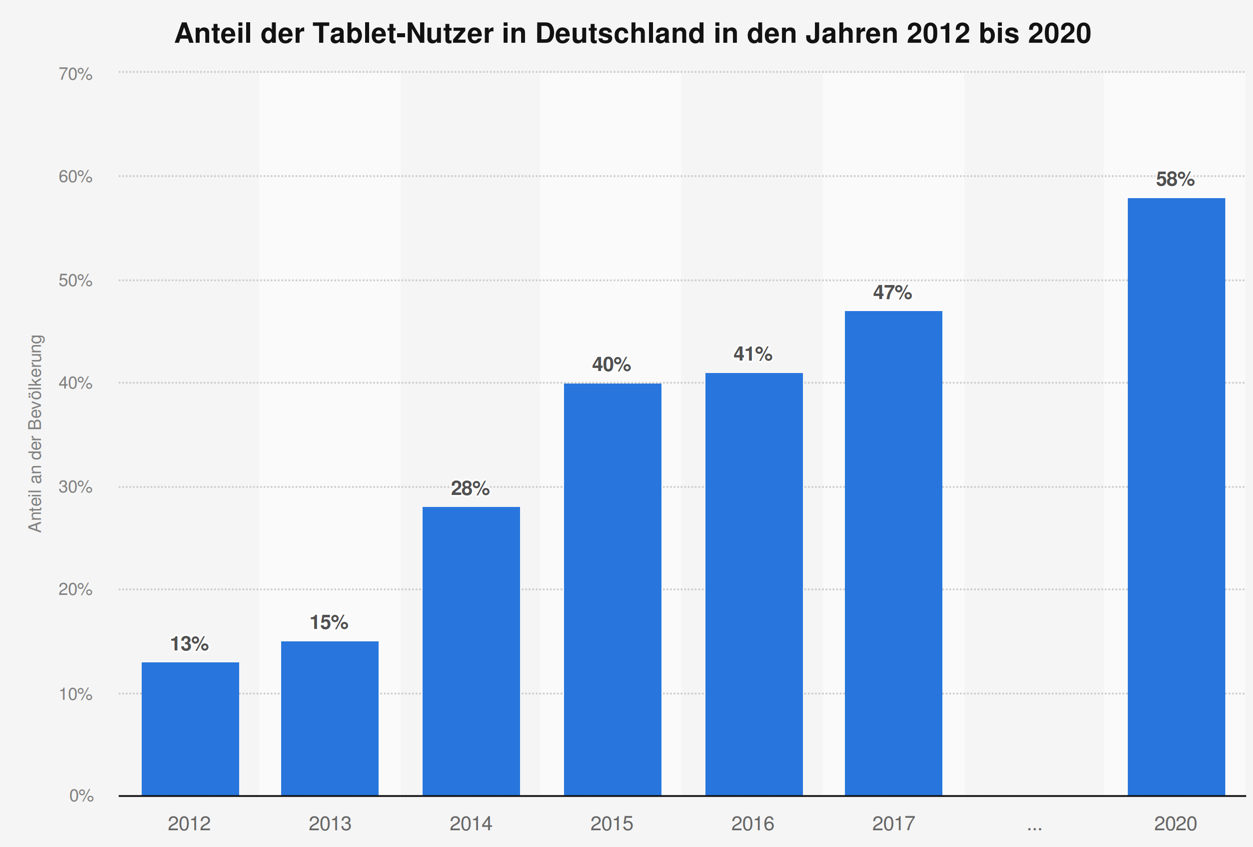
\includegraphics[width=1\textwidth,angle=0]{src/abbildungen/tabletnutzer_2020.png}
    \caption[Quelle: Bitkom, 2020]{Anteil der Tablet-Nutzer:innen in Deutschland von 2012 bis 2020, Quelle: \autocite {Bitkom2021}}
   \label{fig: tablet_nutzer}
   \end{figure}

Dabei zeigt sich, wie viel Potenzial im Online-Handel besteht, wenn ein Kosmetikunternehmen das Interesse potenzieller Kunden und Kundinnen mit Unterstützung einer nahtlosen Verknüpfung der Verkaufskanäle für sich gewinnen kann, wenn dadurch das Einkaufserlebnis kundennäher gestaltet wird. Der Kosmetikhandel kann von diesem Potenzial ebenfalls  profitieren, wenn die Konsumierenden durch richtige Strategieansätze angesprochen werden.

\subsection{Zielsetzung der Arbeit}\label{zielsetzung}
Ziel der Arbeit ist es, Informationen über die Wichtigkeit einer Omni-Channel-Strategie herauszuarbeiten und aufzuzeigen. Ergänzend dazu kann der Prozess zur Einführung eines PIM-Systems mit Hilfe einer Agentur näher beschrieben werden. Ein weiteres Ziel ist es dabei, die Anwendung einer beispielhaften Omni-Channel-Strategie aufzuzeigen.

\subsection{Vorgehensweise}\label{vorgehensweise}
Für die Bachelorthesis hat sich der Autor die folgende Forschungsfrage gestellt.
\newline
Welche spezifischen Herausforderungen und Chancen ergeben sich bei der Implementierung einer Omni-Channel-Strategie im Kosmetikbereich und wie wurden diese von dem Unternehmen BABOR gemeistert \asc{bzw} genutzt?
\newline

Durch Unterstützung von Literaturarbeit wurden zunächst die wichtigsten Punkte für die Anwendung und Umsetzung einer Omni-Channel-Strategie herausgesucht und analysiert. Dabei wurden Chancen und Herausforderungen von Omni-Channel-Strategien aufgedeckt und analysiert.
\clearpage
\section{Begriffsabgrenzung \& Entwicklungen}\label{hauptabschnitt_2}
Da der E-Commerce immer wichtiger wird, ist es für Händler nicht mehr ausreichend, ihre Produkte und Dienstleistungen ausschließlich im stationären Handel anzubieten. Daher wird vom Autor empfohlen, sich regelmäßig mit den neuen Entwicklungen auseinanderzusetzen\footnote{Vgl. \autocite [Online] {Handelsverband2022}}.
So können die Wünsche der Kunden und Kundinnen langfristig erfüllt werden und die Wettbewerbsfähigkeit gegenüber der Konkurrenz stabil bleiben. Auf die Einstiegsmöglichkeiten in den Online-Handel wird im weiteren Verlauf der Arbeit genauer eingegangen.

\subsection{E-Commerce}\label{unterabschnitt_2_1}
\ac{eco} ist eine Abkürzung (zu deutsch: Elektronischer Handel) für den Begriff “Electronic Commerce” und umfasst den Online-Handel, der elektronisch, also im Internet stattfindet. Der Begriff umfasst alle Transaktionen des Handels (Kauf und Verkauf von Waren und Dienstleistungen jeglicher Art), die auf dem elektronischen Weg vollzogen werden\footnote{Vgl. \autocite [S. 19] {Deges2020}}.
Der E-Commerce beinhaltet verschiedene Handelsarten. Wenn ein privater Endkunde in einem Onlineshop einkauft, ist dies eine Business-to-Customer Logik, die oft mit \ac{b2c} abgekürzt wird. Zwischen zwei Unternehmen wird diese Beziehung Business-to-Business oder auch \ac{b2b} bezeichnet\footnote{Vgl. \autocite [S.50] {Heinemann2021}}.
\newline
Der Vertriebsweg sowohl für das B2B- als auch das B2C-Geschäft lässt sich auf zwei verschiedene Arten realisieren. Online-Shops stellen die Art des Direktvertriebs dar. Ein Unternehmen verkauft beispielsweise seine Artikel über einen eigenen Online-Shop.
\newline

Ein weiterer Vertriebsweg ist der Online-Marktplatz. Ein Online-Marktplatz ist eine Webseite, die als Verkaufsplattform dient und auf der sich unterschiedliche Käufer und Verkäufer elektronisch begegnen.
\newline

Als die erfolgreichsten Vertreter:innen dieser Vertriebsart galt lange Zeit das amerikanische Unternehmen eBay, das 1995 gegründet wurde. Vor einigen Jahren wurde eBay von Amazon Marketplace als der erfolgreichste Online-Marktplatz abgelöst\footnote{Vgl. \autocite [Online] {Feldkircher2020}}.
\newline

Durch den Online-Marktplatz-Gigant Amazon entwickelte sich das (\ac{fba}) zu einem beliebten Serviceangebot. Beim FBA zahlt der Verkäufer eine Gebühr an Amazon für Dienstleistungen eines oder mehrerer Produkte. Amazon bietet dann die Produkte auf seinem Portal an und übernimmt sowohl die Produktlagerung als auch den Versand an den Käufer. Für den Verkäufer hat dieses die Vorteile, dass keine Lagerung mehr nötig ist, der Versand erfolgt innerhalb kürzester Zeit ohne jeglichen Aufwand und Amazon bietet die Lieferung an Premiumkunden und Premiumkundinnen versandkostenfrei an.

\subsubsection{Abgrenzung des E-Commerce zum E-Business}\label{unterabschnitt_2_1_1}
Oftmals werden die Begriffe E-Commerce und \ac{ebu} als Synonyme füreinander verwendet. Der E-Commerce beschreibt jedoch nur einen Teil des E-Business und bezieht sich auf den Kauf und Verkauf von Waren und Dienstleistungen über das Internet. E-Commerce ist ein Teilbereich des E-Business, der sich auf die Transaktionen zwischen Unternehmen und Kunden oder Kundinnen konzentriert. E-Commerce umfasst sowohl Business-to-Consumer (B2C), bei dem Unternehmen direkt an Endverbraucher verkaufen, als auch Business-to-Business (B2B), bei dem Unternehmen gegenüber anderen Unternehmen verkaufen.
\newline

Das E-Business umfasst dabei noch weitere Prozesse, die ein Unternehmen über das Internet in Anspruch nehmen kann\footnote{ Vgl. \autocite [S.71] {Meidl2014}}.
\newline
Der Begriff E-Business bezieht sich auf die Verwendung von elektronischen Technologien, um alle Geschäftsprozesse zu optimieren und zu automatisieren. Dies umfasst alle Aktivitäten, die für den Betrieb eines Unternehmens erforderlich sind, wie beispielsweise die interne Kommunikation, die Kundenbetreuung, die Buchhaltung und die Personalverwaltung.


\subsubsection{Entwicklung des E-Commerce}\label{unterabschnitt_2_1_2}
Im Jahr 2021 wurden, wie in den Jahren zuvor, erneut neue Rekordzahlen geschrieben. Es wurden im Bereich E-Commerce durch Online-Einkäufe alleine in Deutschland ca. 87 Milliarden Euro umgesetzt.
\newline
Auch wenn die beiden Pandemie Jahre 2020 und 2021\footnote{Vgl. \autocite [Online] {Wikipedia2019}} nahezu alle Prognosen weit übertroffen haben, gab es im Jahr 2021 verglichen mit dem Vorjahr nochmal einen Anstieg des Umsatzes um mehr als 19\%, was das Potenzial des E-Commerce für die Zukunft nochmal verdeutlicht. Seit 2006 konnte der E-Commerce in Deutschland kontinuierlich steigenden Umsatz verzeichnen. Bei der Auswertung stellt sich heraus, dass die Marktplätze ihre Marktposition weiter ausbauen und vor allem stationäre Händler diese Option nutzen, um im Onlinehandel präsent zu sein.
\newline

Im Geschäftsjahr 2021 wurden von den Käufern über 50\% aller Online Einkäufe über das Smartphone getätigt. Es zeigt sich eine klare Tendenz, dass Verbraucher immer mobiler werden. Für die nächsten Jahre wird prognostiziert, dass der Umsatz kontinuierlich ansteigen wird\footnote{Vgl. \autocite [Online] {Handelsverband2022}}.

\begin{figure}[!ht]
    \centering
    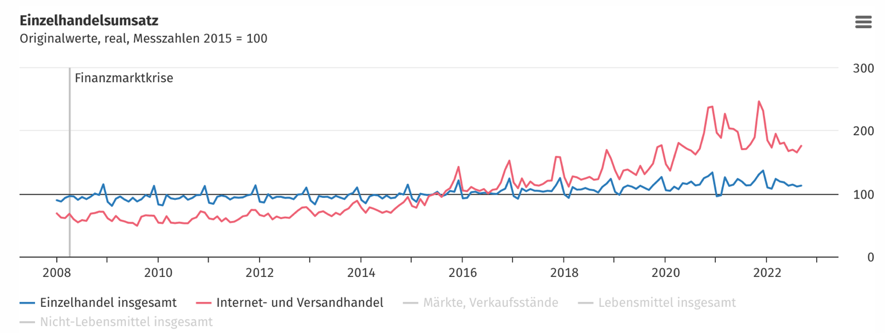
\includegraphics[width=1\textwidth,angle=0]{src/abbildungen/onlineVsEinzelhandel.png}
    \caption[Quelle: Statistisches Bundesamt, 2022]{Umsatzentwicklung von 2008 bis 2022 - Einzelhandel vs. Versandhandel, Quelle: \autocite {Bundesamt2022}}
   \label{fig: Statistisches_Bundesamt}
   \end{figure}

Die vorliegende Grafik visualisiert, dass der Internet- und Versandhandel gegenüber dem Einzelhandel seit 2014 kontinuierlich Konsumierende für sich gewann. Wie die Grafik zudem aufzeigt, übertraf im Jahr 2015 der Umsatz des Internethandels erstmals den des stationären Einzelhandels. Es lässt sich zudem erkennen, dass der Umsatz des Einzelhandels nicht fällt. Allerdings muss auch beachtet werden, dass der Markt stetig wächst und das Wachstum im Einzelhandel hingegen stagniert.


\subsection{Stationärer Einzelhandel}\label{unterabschnitt_2_3}
„Stationärer Handel ist der Sammelbegriff für Handelsbetriebe mit festem Standort“\footnote{Vgl. \autocite [S.23] {Heinemann2011}}.
\newline
Der stationäre Handel ist ein fester Standort, an dem Produkte oder Dienstleistungen zum Kauf angeboten werden. Traditionell wird das Produkt bei einem Kauf direkt mitgenommen.
\newline

Im Optimalfall erleben die Besucher:innen ein Einkaufserlebnis, indem Produkte vor Ort angesehen, taktil wahrgenommen oder auch gerochen werden können. Zudem können sich die Besucher:innen von dem Verkaufspersonal zu den Produkten beraten lassen. Das Kaufverhalten der Besucher:innen wird beeinflusst und der Kaufimpuls gesteigert\footnote{ Vgl. \autocite [S.71] {Buttkus2019}}.
\newline

Ursprungsgemäß sind die Zielgruppe eines stationären Handels Besucher:innen, die zunächst ohne Bedürfnisse den Handel betreten. Während des Besuches wechselt diese Absicht jedoch und es wird für interessant erscheinende Produkte das Kaufempfinden erweckt\footnote{Vgl. \autocite [S.53] {Heinemann2021}}.


\subsubsection{Entwicklung des stationären Einzelhandels}\label{unterabschnitt_2_3_1}
In den letzten Jahrzehnten haben sich die Anforderungen des stationären Einzelhandels verändert. Die ersten Handelsformen waren kleine Einzelhandelsgeschäfte, die Lebensmittel und andere Artikel des täglichen Bedarfs anboten. Die Artikel waren auf die Funktionalität ausgerichtet. Durch die stetige Nachfrage gibt es heute große und moderne Einkaufszentren für verschiedene Branchen\footnote{Vgl. \autocite [S.3] {Jaeger2016}}.
\newline

Wie Abbildung 1 zeigt, entscheiden sich mittlerweile in vielen Branchen immer mehr Verbraucher häufiger für den Online-Einkauf. Einzelhandelsunternehmen erleiden zum Teil negative Nebenwirkungen, wenn Käufer:innen nicht mehr vor Ort ein, sondern sich für den für sie bequemeren Weg entscheiden, online einzukaufen\footnote{Vgl. \autocite [S.11] {Deichner2022}}.
\newline

Auswertungen zufolge bevorzugte im Jahr 2021 etwas weniger als jeder zweite Konsumierende (46 Prozent) den stationären Handel. Daraus lässt sich schließen, dass der Einzelhandel noch immer von hoher Bedeutung ist\footnote{Vgl. \autocite [Online] {Bundesamt2022}}. Auch die gleichbleibenden Umsätze zeigen deutlich auf, dass der stationäre Einzelhandel noch immer von wichtiger Bedeutung ist.
\newline

Der Einzelhandel kann bei vielen von Konsumierenden geforderten Punkten dem E-Commerce allerdings nicht standhalten. Durch den starken Wettbewerb im E-Commerce wird der Preis von großen Unternehmen gedrückt, wodurch viele kleine Unternehmen nicht wettbewerbsfähig agieren können und um ihre Existenz kämpfen müssen.
\newline

Für den Einzelhandel besteht die Herausforderung, dynamisch agieren und schnellstmöglich auf Veränderungen reagieren zu können. Die Corona-Pandemie beispielsweise traf viele kleinere Unternehmen, weil diese zum Teil über Monate aufgrund der Lockdowns ihre Geschäfte nicht öffnen durften. Online-Shops hingegen sind dauerhaft erreichbar und Pakete kommen in der Regel innerhalb weniger Werktage bei dem Kunden oder der Kundin an. An diese Flexibilität und Bequemlichkeit gewöhnen sich Konsumierende schnell, wenn ein gesuchtes Produkt über Suchmaschinen von vielen Online-Shops angeboten wird. Durch diese dauerhafte Erreichbarkeit und Verfügbarkeit eines Produkts werden neue Anforderungen an den Einzelhandel gestellt. Dadurch steigt der Anspruch der Kundschaft, der Einzelhandel allerdings wird diesem Anspruch nicht gerecht und klafft bei vielen Kunden mit der Zufriedenheit auseinander\footnote{Vgl. \autocite [S.3] {Jaeger2016}}.

\begin{figure}[!ht]
    \centering
    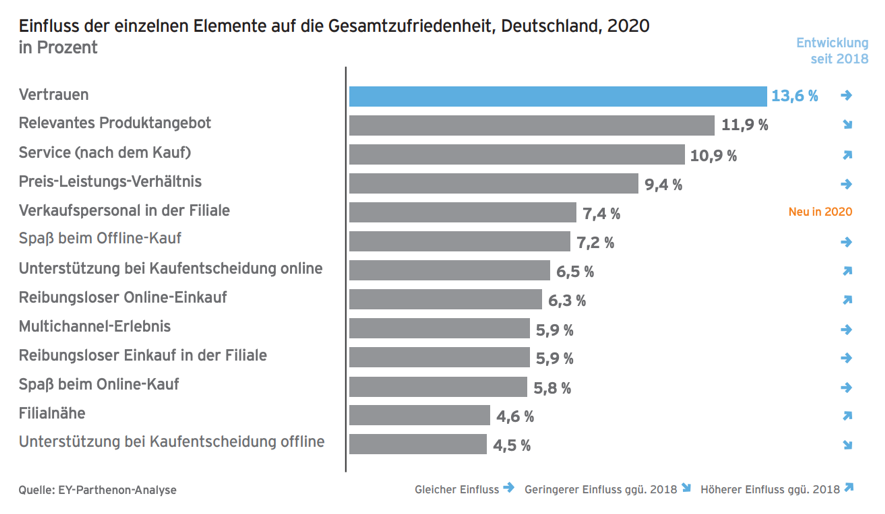
\includegraphics[width=1\textwidth,angle=0]{src/abbildungen/gesamtzufriedenheit_verbraucher.png}
    \caption[Quelle: EY-Parthenon-Analyse, 2020]{EY-Parthenon-Analyse, Quelle: \autocite {EYParthenon2020}}
   \label{fig: Quelle: EY-Parthenon-Analyse 2020}
   \end{figure}

Bei dieser repräsentativen Studie wurden Konsumierende in mehreren europäischen Ländern und in den USA nach ihrer Wahrnehmung des Leistungsversprechens befragt.
\newline
Es ist eine klare Tendenz erkennbar, dass aus Kundensicht beliebte Faktoren für die Kundenzufriedenheit wie Produktangebot oder Preis-Leistungs-Verhältnis von großen Unternehmen im Internet einfacher anzubieten sind, als von Einzelhandelsunternehmen.
Auch bei der Qualifikation des Verkaufspersonals oder einem ansprechenden Ambiente herrscht bei vielen Einzelhandelsunternehmen Nachholbedarf.
\newline

Unternehmen sollten zum Beispiel den Vorteil nutzen, mit guten Verkaufsberatungen vor Ort die Zufriedenheit des Kunden zu wecken und diesen in den Mittelpunkt zu stellen. Für den stationären Einzelhandel wäre es wichtig, mit Freundlichkeit und Expertise den Kunden zu überzeugen und beim Kaufen zu unterstützen.


\subsection{Der Begriff Kosmetik}\label{unterabschnitt_2_5}
Der Begriff Kosmetik bezieht sich auf Produkte und Dienstleistungen, die zur Verbesserung des Aussehens und der Schönheit von Haut, Haaren und Nägeln verwendet werden. Kosmetikprodukte umfassen in der Regel Hautpflegeprodukte, dekorative Kosmetik (Make-up), Parfüm, Haarpflegeprodukte und Produkte für die Nagelpflege.
\newline

Hautpflegeprodukte umfassen verschiedene Arten von Cremes, Lotionen, Serums und Masken, die dazu verwendet werden, die Haut zu pflegen, zu befeuchten und zu schützen. Sie können auf verschiedene Hauttypen und -bedürfnisse abgestimmt sein und bestehen aus verschiedenen Inhaltsstoffen, darunter Feuchthaltemittel, Fette und Öle, Vitamine und Pflanzenextrakte\footnote{Vgl. \autocite [S. 11] {Umbach2012}}.
\newline

Make-up umfasst verschiedene Arten von Produkten, die verwendet werden, um das Aussehen der Haut, der Augen, der Lippen und der Wangen zu verbessern. Dazu gehören beispielsweise Foundations, Concealer, Rouge, Lidschatten, Mascara und Lipgloss. Make-up kann in verschiedenen Formen erhältlich sein, darunter Flüssigkeiten, Cremes und Pulver.
Parfüm ist ein Duftstoff, der in einer Flüssigkeit oder einer Creme suspendiert ist und zur Verbesserung des Körpergeruchs verwendet wird. Es gibt viele verschiedene Arten von Parfüm, die auf verschiedene Weise hergestellt werden und unterschiedliche Duftnoten aufweisen.
\newline

Haarpflegeprodukte umfassen verschiedene Arten von Shampoo, Conditioner, Haaröl und anderen Produkten, die zur Pflege und Styling von Haaren verwendet werden. Sie können auf verschiedene Haartypen und -bedürfnisse abgestimmt sein und bestehen aus verschiedenen Inhaltsstoffen, darunter Feuchthaltemittel, Proteinen, Ölen und Pflanzenextrakten.
Produkte für die Nagelpflege umfassen verschiedene Arten von Lacken, Reinigern und anderen Produkten, die zur Pflege und Verschönerung von Nägeln verwendet werden. Dazu gehören beispielsweise Nagelfeile, Nagelknipser, Nagelpflegelacke und Nagelhärter.
\newline

Bei der Herstellung von Kosmetikprodukten müssen rechtliche Grundlagen erfüllt werden. In Europa unterliegen Kosmetikprodukte der \ac{eu}-Kosmetikverordnung, die Anforderungen an die Sicherheit, Kennzeichnung und Notifizierung von Produkten festlegt. In anderen Regionen der Welt gelten hingegen andere Regelungen. Es ist wichtig, sich über die geltenden Gesetze und Vorschriften in dem Land zu informieren, in dem das Produkt hergestellt und verkauft werden soll\footnote{Vgl. \autocite [online] {Haendlerbund2013}}.

\subsubsection{Entwicklung der Kosmetikbranche in Deutschland}\label{unterabschnitt_2_5_1}
Mit Blick auf die vergangenen 10 Geschäftsjahre ist das Marktvolumen von Kosmetik- und Körperpflegeprodukten, mit Ausnahme der Pandemiejahre 2020-2021, kontinuierlich angestiegen und bewegte sich 2013 bei 13,6 Milliarden Euro Umsatz und im Jahr 2021 bei knapp 16 Milliarden Euro Umsatz. Für das Jahr 2022 wurde im August 2022 ein Jahresumsatz von 15,75 Milliarden prognostiziert. Aufgrund der Ausbreitung des COVID-19-Virus folgte deutschlandweit die vorübergehende Schließung vieler stationärer Geschäfte. In dieser Zeit konnten viele Unternehmen zum Teil über Monate keinen Umsatz durch das Ladengeschäft generieren. In den Zahlen machte sich dies deutlich, indem der Umsatz im Einzelhandel in der Kosmetikbranche über diesen Zeitraum um 15 Prozent sank\footnote{Vgl. \autocite [Online] {statista2022}}.
\newline

Ein Großteil der Kosmetikprodukte kauften die Kunden während dieser Zeit über den Online-Handel.
\newline
Gezwungenermaßen waren Unternehmen dazu aufgefordert, die Sicht auf das Online-Geschäft zu erweitern, um die Kundenbedürfnisse zufrieden zu stellen und den Umsatz möglichst aufrechtzuerhalten.
\newline
Die Kosmetikbranche hat sich im Laufe der Pandemie den Herausforderungen gestellt und als widerstandsfähig erwiesen.
\newline

Durch die Revolution des Online-Geschäfts und vieler neuer Technologiemöglichkeiten wie dem sprachbasiertem Online-Einkauf über Sprachassistenten wie Alexa wurden in den vergangenen Jahren neue Einkaufsmöglichkeiten gesetzt, wodurch automatisch auch die Kundenanforderungen gestiegen sind und eine neue Erwartungshaltung entstanden ist.
\newline

Eine schlechte Onlinepräsenz nimmt den Unternehmen die Reichweite, um Kunden für sich zu gewinnen und Kundenbedürfnisse zu befriedigen.
\newline

Die Entwicklung zum branchenübergreifenden Online- und Versandhandel ist jedoch nicht erst seit Corona aktuell, sondern wie in Punkt 2.1.2. beschrieben, ein Prozess, der kontinuierlich verlief. Die Corona Pandemie war ein weiterer Indikator, wie wichtig es für Unternehmen ist, die neuen Technologien gewinnbringend zu nutzen und als Unternehmen zu wachsen.
\newline
Mittlerweile kann der E-Commerce als passende Ergänzung zum Online-Shop genutzt werden. Der E-Commerce dient nicht nur als gute Erweiterung, sondern bietet auch neue Möglichkeiten, sodass beide Handelsarten erfolgreich miteinander kombinieren können.
\newline

Auch in Bezug auf die Herstellung der Kosmetikprodukte veränderten sich durch die Sichtweise der Konsumierenden in den letzten 10 Geschäftsjahren die Anforderungen für die Herstellung der Kosmetikprodukte. Es wird vermehrt auf Produkte bestehend aus zwei Ansätzen gesetzt. Diese bestehen zum einen aus der Wirkstoffkosmetik und zum anderen aus der Naturstoffkosmetik. Produkte aus der Wirkstoffkosmetik sorgen nachweislich dafür, die Haut zu verbessern. Naturstoffkosmetik Produkte basieren auf rein pflanzlicher Herstellung. Der Trend der Konsumierenden verläuft eindeutig in die Richtung, vegane Produkte zu kaufen. Aus diesem Grund sind die Unternehmen dazu aufgefordert, Produkte aus der Naturstoffkosmetik anzubieten\footnote{Vgl. \autocite [Online] {Verbraucherzentrale2022}}.


\subsection{Grundlagen der verschiedenen Handelsarten}\label{hauptabschnitt_2_grundlagen}
Um sich dem Phänomen des Omni-Channel-Retailing (=Einzelhandel) zu nähern, ist es hilfreich, den Begriff zu definieren und abzugrenzen. Sowohl in den Medien als auch in der Praxis werden in diesem Zusammenhang oft die Begriffe Multi-Channel- und Cross-Channel-Handel genutzt. Es handelt sich hierbei zwar um ähnliche Handelsformate, allerdings bauen diese aufeinander auf und sind jeweils von ihrem Vorgänger abzugrenzen.

\newpage

\begin{figure}[!ht]
    \centering
    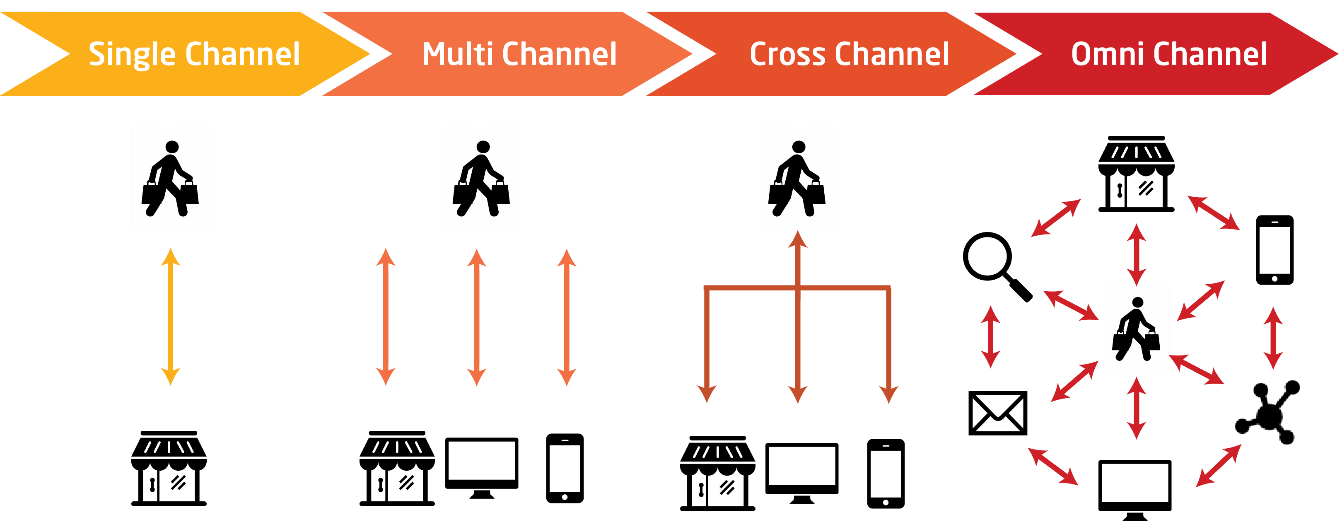
\includegraphics[width=0.95\textwidth,angle=0]{src/abbildungen/verkaufskanaele.png}
    \caption[Quelle: Multi-Channel, Omni-Channel oder Personalisierung, 2022]{Entwicklung der verschiedenen Geschäftsmodelle in Anlehnung an Talin , Quelle: \autocite {Talin2022}}
   \label{Onlineshopping_smartphone}
   \end{figure}
\newline

Im Folgenden wird Geschichtliches zu den Begriffen erläutert und wie diese Handelsformate entstanden sind. Zudem werden in diesem Zusammenhang benutzte Fachbegriffe erläutert.

\subsubsection{Single-Channel-Handel}\label{unterabschnitt_2_2_1}
Übersetzt bedeutet der Begriff Single-Channel „Einzel-Kanal“. Bezogen auf den Handel wird bei Single-Channel-Strategien von Händlern gesprochen, die einzig und allein über einen Vertriebskanal verfügen. Dies kann zum Beispiel der Online-Shop alleine oder ein stationärer Verkaufsladen sein. Erwähnenswert ist, dass die Online-Pure-Player, die „nur“ über einen Online-Marktplatz verfügen, ebenfalls zu der Kategorie des Single-Channel-Anbieters zählen. Weitere Beispiele sind zum Beispiel ein Schreibwarenladen, der lediglich innerhalb dessen Geschäfts die Waren verkauft.


\subsubsection{Multi-Channel-Handel}\label{unterabschnitt_2_2_2}
Multi-Channel-Retailing (Handel über mehrere Vertriebswege) zeichnet aus, dass ein Unternehmen Besucher:innen und potenzielle Kunden und Kundinnen über mehr als nur einen Verkaufskanal bzw. Vertriebsweg erreichen kann. So soll die Erreichbarkeit des Unternehmens an die Kundschaft erhöht und die Umsätze gesteigert werden\footnote{Vgl. \autocite [S.20] {Wirtz2022}}.
Ein Unternehmen bietet beim Einsatz einer Multi-Channel-Strategie verschiedene Vertriebskanäle an.
\newline

Ein Vertriebskanal oder Verkaufskanal lässt sich zunächst in zwei Kategorien unterteilen. Bei der Art des direkten Vertriebskanals verkauft ein Unternehmen seine Produkte direkt an die Konsumierenden bzw. Verbraucher:innen. Beispiele sind unter anderem der direkte Vertrieb vor Ort an den Endkunden oder über den eigenen Online-Shop. Bei indirekten Vertriebskanälen sind Zwischenhändler involviert, die dabei unterstützen sollen, einen größeren Kundenstamm für das Unternehmen zu erreichen. Beispiele sind Einzelhändler, Großhändler oder Online-Marktplätze wie Amazon\footnote{Vgl. \autocite [Online] {GisclardBiondi2021}}.
\newline

Der Begriff Multi-Channel-Retailing wurde vor knapp 140 Jahren zum ersten Mal in diesem Kontext genutzt, als die kanadische Warenhauskette Timothy Eaton den ersten Versandkatalog weltweit herausgebracht hat\footnote{Vgl. \autocite [Online] {Santink2015}}.
\newline

Der Versandhändler Otto hat 2021/2022 einen Jahresumsatz von über 16 Milliarden Euro verbucht und gehört heutzutage nicht nur zu den erfolgreichsten Onlinehändlern in Europa, sondern ist einer dieser Giganten, der die Stärken des Multichannel-Retailing bereits 1949 mit seinem ersten Versandkatalog erkannt und im Laufe der Zeit perfektioniert hat\footnote{Vgl. \autocite [Online] {Otto2022}, \autocite [Online] {Rabe2022}}.
\newline

Zudem kam neben dem Versandhandel seit 1995 der Onlinehandel hinzu, der sich durch die Digitalisierung, mit dem Beginn der Erfindung des Internets, weiter verändert hat. Bei vielen Unternehmen folgte im Laufe der Jahre ein Umdenken der Unternehmensstrategie, weil der Wettbewerb nicht mehr nur regional vertreten war, sondern sich global verlagerte. Dadurch, dass der Onlinehandel neue Maßstäbe setzen konnte, die von nun an die Bedürfnisse der Kunden deckten, entwickelte sich der Onlinehandel für den stationären Handel zu einer großen Konkurrenz.
\newline

Große Online Pure Player\footnote{Vgl. \autocite [Online] {Deges2020a}} wie Alibaba, Amazon oder eBay, die ihren Vertrieb ausschließlich über den Distanzhandel\footnote{Vgl. \autocite [Online] {Schneider2018}} betreiben, können ihren Kunden eine größere Produktauswahl zu besseren Konditionen anbieten. Eine rund um die Uhr Erreichbarkeit mit einem 24/7 Service (24 Stunden am Tag und 7 Tage pro Woche verfügbar) ist keine Seltenheit mehr. Von der Bestellung zur Versandabwicklung bis vor die Tür vergehen in der Regel nur wenige Tage.\footnote{Vgl. \autocite [S.17] {Vallee2018}}
\newline

Eine mögliche Umsetzungsart, weiterhin wettbewerbsfähig zu sein, ist für viele Einzelhandelsunternehmen die Einsetzung einer Multi-Channel-Strategie, indem sie zusätzlich zu ihrem stationären Handel einen Onlineshop aufbauen.


\subsubsection{Cross-Channel-Handel}\label{unterabschnitt_2_2_3}
Vor einem Jahrzehnt stellten sich viele Unternehmen noch die Frage, ob es notwendig sei, auch einen Onlineshop zu betreiben, um den Kundenstamm zu erweitern oder konkurrenzfähig zu bleiben. Heute stellen sich diese Unternehmen viel mehr die Frage, ob das Filialgeschäft mit dem Onlinekanal besser verknüpft werden muss. Beide Fragen sind klar mit ja zu beantworten, denn wenn ein Unternehmen es selbst nicht früh genug in die Hand nimmt, finden sich Konkurrenzunternehmen, die nicht zögern und Kundenbedürfnisse für die Zukunft besser befriedigen können.
\newline

2016 zeigte das \ac{ehi} Retail Institut mit einer Studie, wie fortgeschritten der Trend zum Onlinehandel bereits ist\footnote{Vgl. \autocite [S.17] {Hofacker2016}}.  Mehr als 70 Prozent der befragten Handelsunternehmen schätzten bereits 2016 das Click \& Collect Konzept, bei der die Ware online bestellt werden kann und in der nächstgelegenen Filiale abgeholt werden kann, als wichtig ein.
\newline

Über zwei Drittel der Befragten empfinden auch die Online-Bestandsabfrage als sehr sinnvoll ein, ebenso wie das Angebot eines Instore-Returns. Ein Instore-Return ist ein über den Onlineshop gelieferter Artikel, der vor Ort wieder returniert werden kann.
\newline

Bei der Cross-Channel-Integration spielt die Vernetzung der Online- und Offlinekanäle eine entscheidende Rolle.
\newline
Das Cross-Channel-Retailing erweitert das Multi-Channel-Verfahren und man spricht von Cross-Channel-Integration, sobald die ersten Verkaufskanäle miteinander verknüpft sind. Für Kunden entsteht dadurch die Möglichkeit, das Einkaufserlebnis kanalübergreifend zu gestalten, indem der Einkauf über verschiedene Verkaufskanäle abgewickelt werden kann. Darin enthalten sind zum Beispiel die Bestellung als Click \& Collect aufzugeben. Weitere Begriffe sind das \ac{fba} oder auch der \ac{b2b}-Handel
\newline

Mit der Verknüpfung der Verkaufskanäle gibt ein Unternehmen aber nicht nur den Kunden neue Möglichkeiten. Mitarbeiter können unter anderem Produkt- oder Kundendaten abfragen und dem Kunden so ein verbessertes Feedback über Produktfragen bieten.


\subsubsection{Omni-Channel-Handel}\label{unterabschnitt_2_2_4}
Der Begriff „omni“ stammt aus dem Lateinischen. Omni bedeutet so viel wie „alle“, „alles“, oder „ganz“\footnote{Vgl. \autocite [Online] {Wortbedeutung.info2022}}.
\newline
Wie bereits in Punkt 3 beschrieben, legt das Single-Channel-Marketing eine Basis für alle anderen Channel Arten, die aufeinander aufbauen. Um die Wichtigkeit zu verdeutlichen, ist Omni-Channel-Retailing zwar eine Weiterentwicklung des Multi-Channel-Verfahrens, doch diese ist grundlegend und damit ein wesentlicher Teil des Omni-Channel-Retailing.
\newline

Im Omni-Channel-Retailing werden die Daten der verschiedenen Kanäle miteinander verbunden und zentralisiert, sodass alle Plattformen perfekt aufeinander abgestimmt sind und keine Konkurrenz entsteht, sondern ein gesundes Zusammenspiel entsteht.
\newline
Die Umsetzung der Omni-Channel-Strategie wird sehr stark auf die Kundenbedürfnisse abgestimmt, um die Zufriedenheit der Kunden und Kundinnen so hoch wie möglich zu gewährleisten.
\newline
Durch die Digitalisierung haben sich die Konsumierenden mittlerweile stark an das Online-Shopping gewöhnt und oft entsteht dabei auch die zum Teil unbewusste Parallelnutzung von mehreren Vertriebskanälen, um zum Beispiel Preise zwischen Marktplätzen und dem Online-Shop zu vergleichen. Beim Omni-Channel-Retailing soll die Infrastruktur so angepasst werden, dass ein angenehmes Kauferlebnis entstehen kann.
\newline

Durch die Weiterentwicklung neuer Technologien und einer daraus resultierenden steigenden Anzahl an Online Einkäufen, die über Smartphones abgewickelt werden, findet die Anwendung einer Omni-Channel-Strategie im E-Commerce bei vielen Unternehmen immer häufiger Anklang.
\newline

Dabei findet sowohl eine Verschmelzung der Sortiments- und Verkaufsprozesse, als auch der Systeme und Datenbanken statt. Beim Omni-Channel-Retailing werden die Produkte von einem Unternehmen parallel über verschiedene Vertriebswege angeboten, zum Beispiel über den Online-Shop und eine App oder zusätzlich direkt im stationären Handel.
\newline

Der große Vorteil ist dabei, dass die Steuerung all dieser Kanäle durch die Verknüpfung von Verkaufsprozessen, Datenbanken und Systemen zentriert erfolgt. Es gibt also eine Schnittstelle, die die Verkaufskanäle miteinander synchronisiert, sodass ein nahtloser Übergang von einem Vertriebskanal in den anderen Vertriebskanal problemlos möglich ist, ohne dabei das Einkaufserlebnis des Konsumierenden einzuschränken.
\newline

Eine Customer Journey ist eine Kundenreise, die das Einkaufserlebnis eines Verbrauchers bis zum Kauf widerspiegelt\footnote{Vgl. \autocite [S. 21] {Boeckenholt2018}}.  Der Wechsel zwischen den Vertriebskanälen soll dadurch reibungslos und bequem ablaufen, ohne dass Einschränkungen oder Nachteile für den Kunden oder die Kundin entstehen.
\newline

Omni-Channeling zeichnet auch aus, dass der Kunde oder die Kundin zu jeder Zeit und an jedem Ort jeden verfügbaren Kanal in ein Kaufentscheidungsprozess einsteigen kann. Für das Unternehmen besteht dadurch die Möglichkeit, 24 Stunden am Tag die eigenen Artikel verkaufen zu können.
\newline

Dadurch erhält der Konsumierende den Vorteil, sich nicht für einen Vertriebskanal entscheiden zu müssen und ggf. sogar zwei Vertriebskanäle parallel zu nutzen\footnote{Vgl. \autocite [S. 20] {Heinemann2013}}.
Dieser Vorgang des Einkaufens wird als Omni-Channeling oder auch Omni-Channel-Nutzung bezeichnet. Der Einsatz von Omni-Channel-Retailing verfolgt das Ziel, die Customer Journey des Kunden oder der Kundin so angenehm wie möglich zu gestalten und das Einkaufserlebnis über mehrere Vertriebskanäle hinweg zu vereinheitlichen. Ein nahtloser Wechsel zwischen den Vertriebskanälen lässt die Zufriedenheit des Verbrauchers steigen. Diese Zufriedenheit spiegelt sich wider, indem der Verbraucher das Produkt bei dem Unternehmen kauft und im besten Fall für weitere Einkäufe wieder zum Anbieter zurückkehrt.
\newline

Zusätzlich zu dem stationären Handel und dem Onlinehandel als interaktive Vertriebskanäle des Multi-Channels gehören beim Omni-Channel ebenfalls noch die mobilen Vertriebskanäle hinzu, die vorzugsweise über Smartphone, Computer oder Tablet über eine App genutzt werden. Beispiele sind der Verkauf über soziale Medien, Marktplätze oder andere Kommunikationskanäle wie Printmedien, Radio oder Fernsehen.
\newline

Anders als bei Multi-Channel-Retailing werden beim Omni-Channel-Retailing die Verkaufsziele jedoch kanalübergreifend gesetzt.
\clearpage
\section{Omni-Channel}\label{hauptabschnitt_3}

\subsection{Welche Rolle spielt E-Commerce im Omni-Channel?}\label{unterabschnitt_3_1}
E-Commerce spielt eine wichtige Rolle im Omni-Channel-Ansatz, bei dem Unternehmen ihre Kunden und Kundinnen  über mehrere Kanäle hinweg ansprechen und interagieren. E-Commerce ist ein wichtiger Kanal, um Kunden und Kundinnen  online zu erreichen und ihnen Produkte und Dienstleistungen anzubieten.
\newline
Bei einem Omni-Channel-Ansatz besteht für Unternehmen ein Nebenziel darin, mittelfristig die Bekanntheit der eigenen Marke durch die Nebenwirkungen des Omni-Channel-Marketings auszubauen. Durch neue Point-of-Sale Möglichkeiten werden die Produkte und Dienstleistungen online angeboten. Dies ermöglicht es ihnen, die Kunden und Kundinnen auf verschiedenen Kanäle zu erreichen, zum Beispiel über ihre eigene Website, Social-Media-Plattformen oder Marktplätze wie Amazon.
\newline
Ein \ac{pos} ist ein Verkaufspunkt bzw. ein Ort, der es den Kunden und Kundinnen ermöglicht, ein Produkt zu kaufen. Im Allgemeinen bezieht sich der POS auf physische Verkaufsstellen, wie z.B. Ladengeschäfte, der POS kann sich aber auch auf Online-Verkaufsstellen, wie einen Marketplace oder einen Online-Shop beziehen\footnote{Vgl. \autocite [Online] {Kenning2018}}.
POS-Systeme bestehen aus Hardware und Software, die es dem Verkäufer ermöglichen, Artikel zu scannen, Zahlungen zu akzeptieren und Berichte zu erstellen und sie können zudem in andere Systeme wie Lagerverwaltung, Buchhaltung und CRM integriert sein.
\newline

E-Commerce ermöglicht es Unternehmen auch, ihre Kunden und Kundinnen über verschiedene Geräte hinweg anzusprechen, wie zum Beispiel Desktop-Computer, Laptops, Tablets und Smartphones. Auf diese Weise können Unternehmen ihre Kunden und Kundinnen  jederzeit und überall erreichen und ihnen eine nahtlose Einkaufserfahrung bieten.
\newline
Im Omni-Channel-Ansatz arbeiten E-Commerce und andere Kanäle wie der stationäre Handel, Kataloge und andere Marketing- und Verkaufskanäle zusammen, um eine umfassende Kundenerfahrung zu bieten. Kunden und Kundinnen  können zum Beispiel online recherchieren und dann im Ladengeschäft kaufen, oder umgekehrt. Unternehmen können auch eine integrierte Kundenbeziehung über mehrere Kanäle hinweg aufbauen und pflegen, indem sie Informationen und Interaktionen über alle Kanäle hinweg verfolgen und nutzen.
\newline

Eine repräsentative Studie des Handelsverband Deutschland von 2021 untermauert, dass der Online Einkauf in Deutschland nicht nur steigt, sondern dass der Einkauf über Smartphones immer häufiger genutzt wird und in den letzten Jahren kontinuierlich steigt. Diese Studie zeigt allerdings auch, dass Deutschland marketingtechnisch noch nicht auf dem Entwicklungsstand ist, wie es zum Beispiel Länder aus Asien sind (z.B. China oder Südkorea). In Deutschland zweifeln viele Unternehmen noch, innovative Projekte mit der Nutzung von Künstlicher Intelligenz in ihr Unternehmen zu integrieren. Rund 13\% der Unternehmen wenden demnach KI in Deutschland aktiv mindestens in einzelnen Bereichen an. Es sind zudem rund 15\% der restlichen Unternehmen bereit, KI in Zukunft einzuplanen, während über 72\% ohne KI planen\footnote{Vgl. \autocite [Online] {Handelsverband2021}}.
\begin{figure}[!ht]
    \centering
    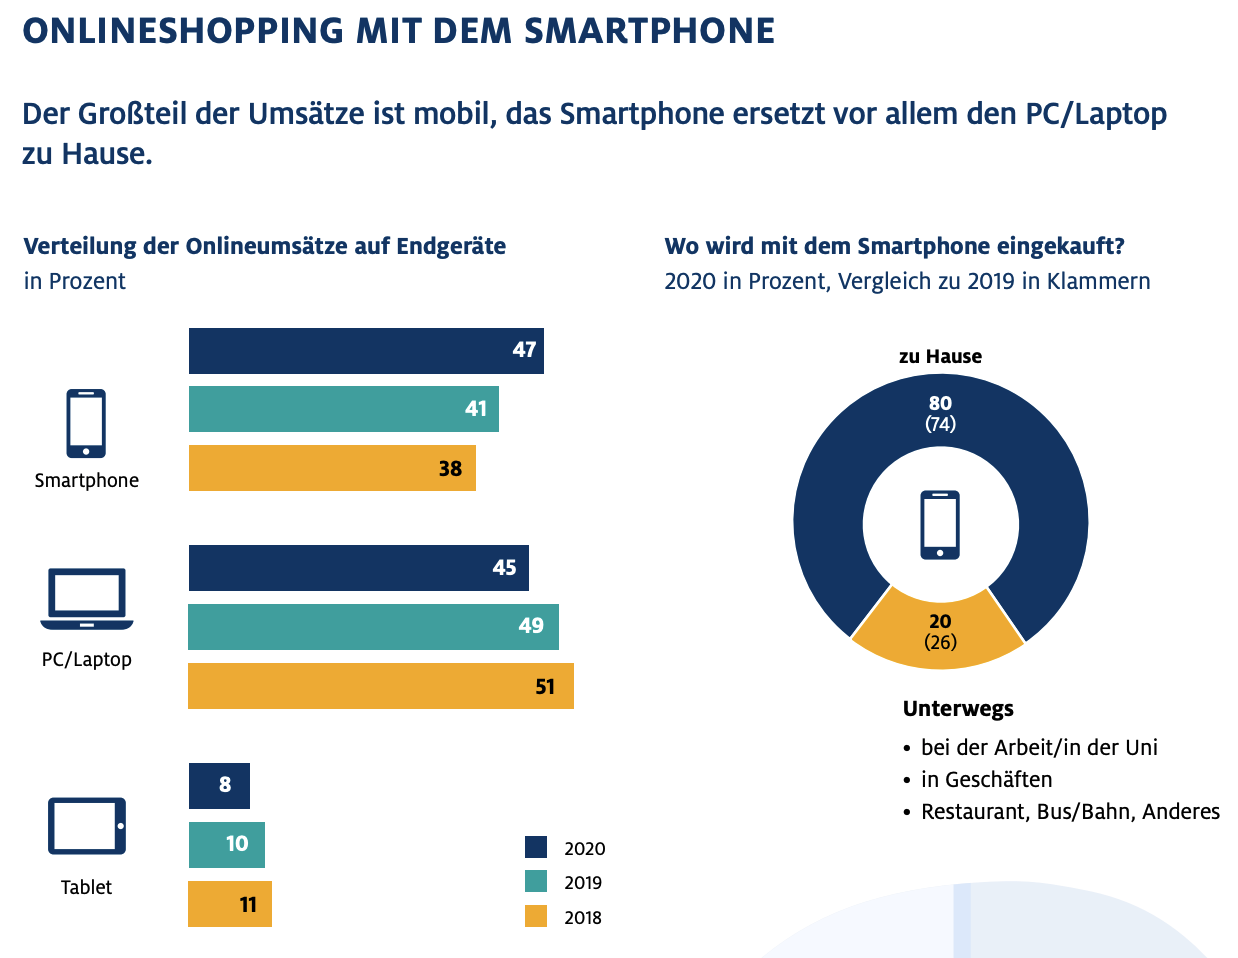
\includegraphics[width=0.95\textwidth,angle=0]{src/abbildungen/Shopping_smartphone.png}
    \caption[Quelle: HDE Deutschland Handelsverband - Marktentwicklung im Online-Handel, 2021]{Vgl.: Onlineshopping mit dem Smartphone, Quelle: \autocite {Handelsverband2021}}
   \label{Onlineshopping_smartphone}
   \end{figure}


\subsection{Wichtigkeit der Customer Journey}\label{unterabschnitt_3_2}
Als einer der ersten Menschen stellte Elmo Lewis bereits 1898 ein vier Stufen Modell auf, bei dem die Kunden und Kundinnen  vier Phasen bis zum Kauf des Produktes durchlaufen. Das sogenannte AIDA-Modell\footnote{Vgl. \autocite [Online] {Heubel2019}} beginnt damit, dass der Kunde oder die Kundin zum Beispiel durch Werbung auf ein Produkt aufmerksam gemacht werden soll (Awareness). Daraus resultiert ein Interesse des Betrachters, der sich mit dem Produkt oder der Werbung beschäftigt (Interest). Im dritten Schritt ist der Betrachter überzeugt von dem Produkt und hat den Wunsch, das Produkt zu kaufen (Desire).  In der vierten Phase wird das Produkt gekauft (Action).
\begin{figure}[!ht]
    \centering
    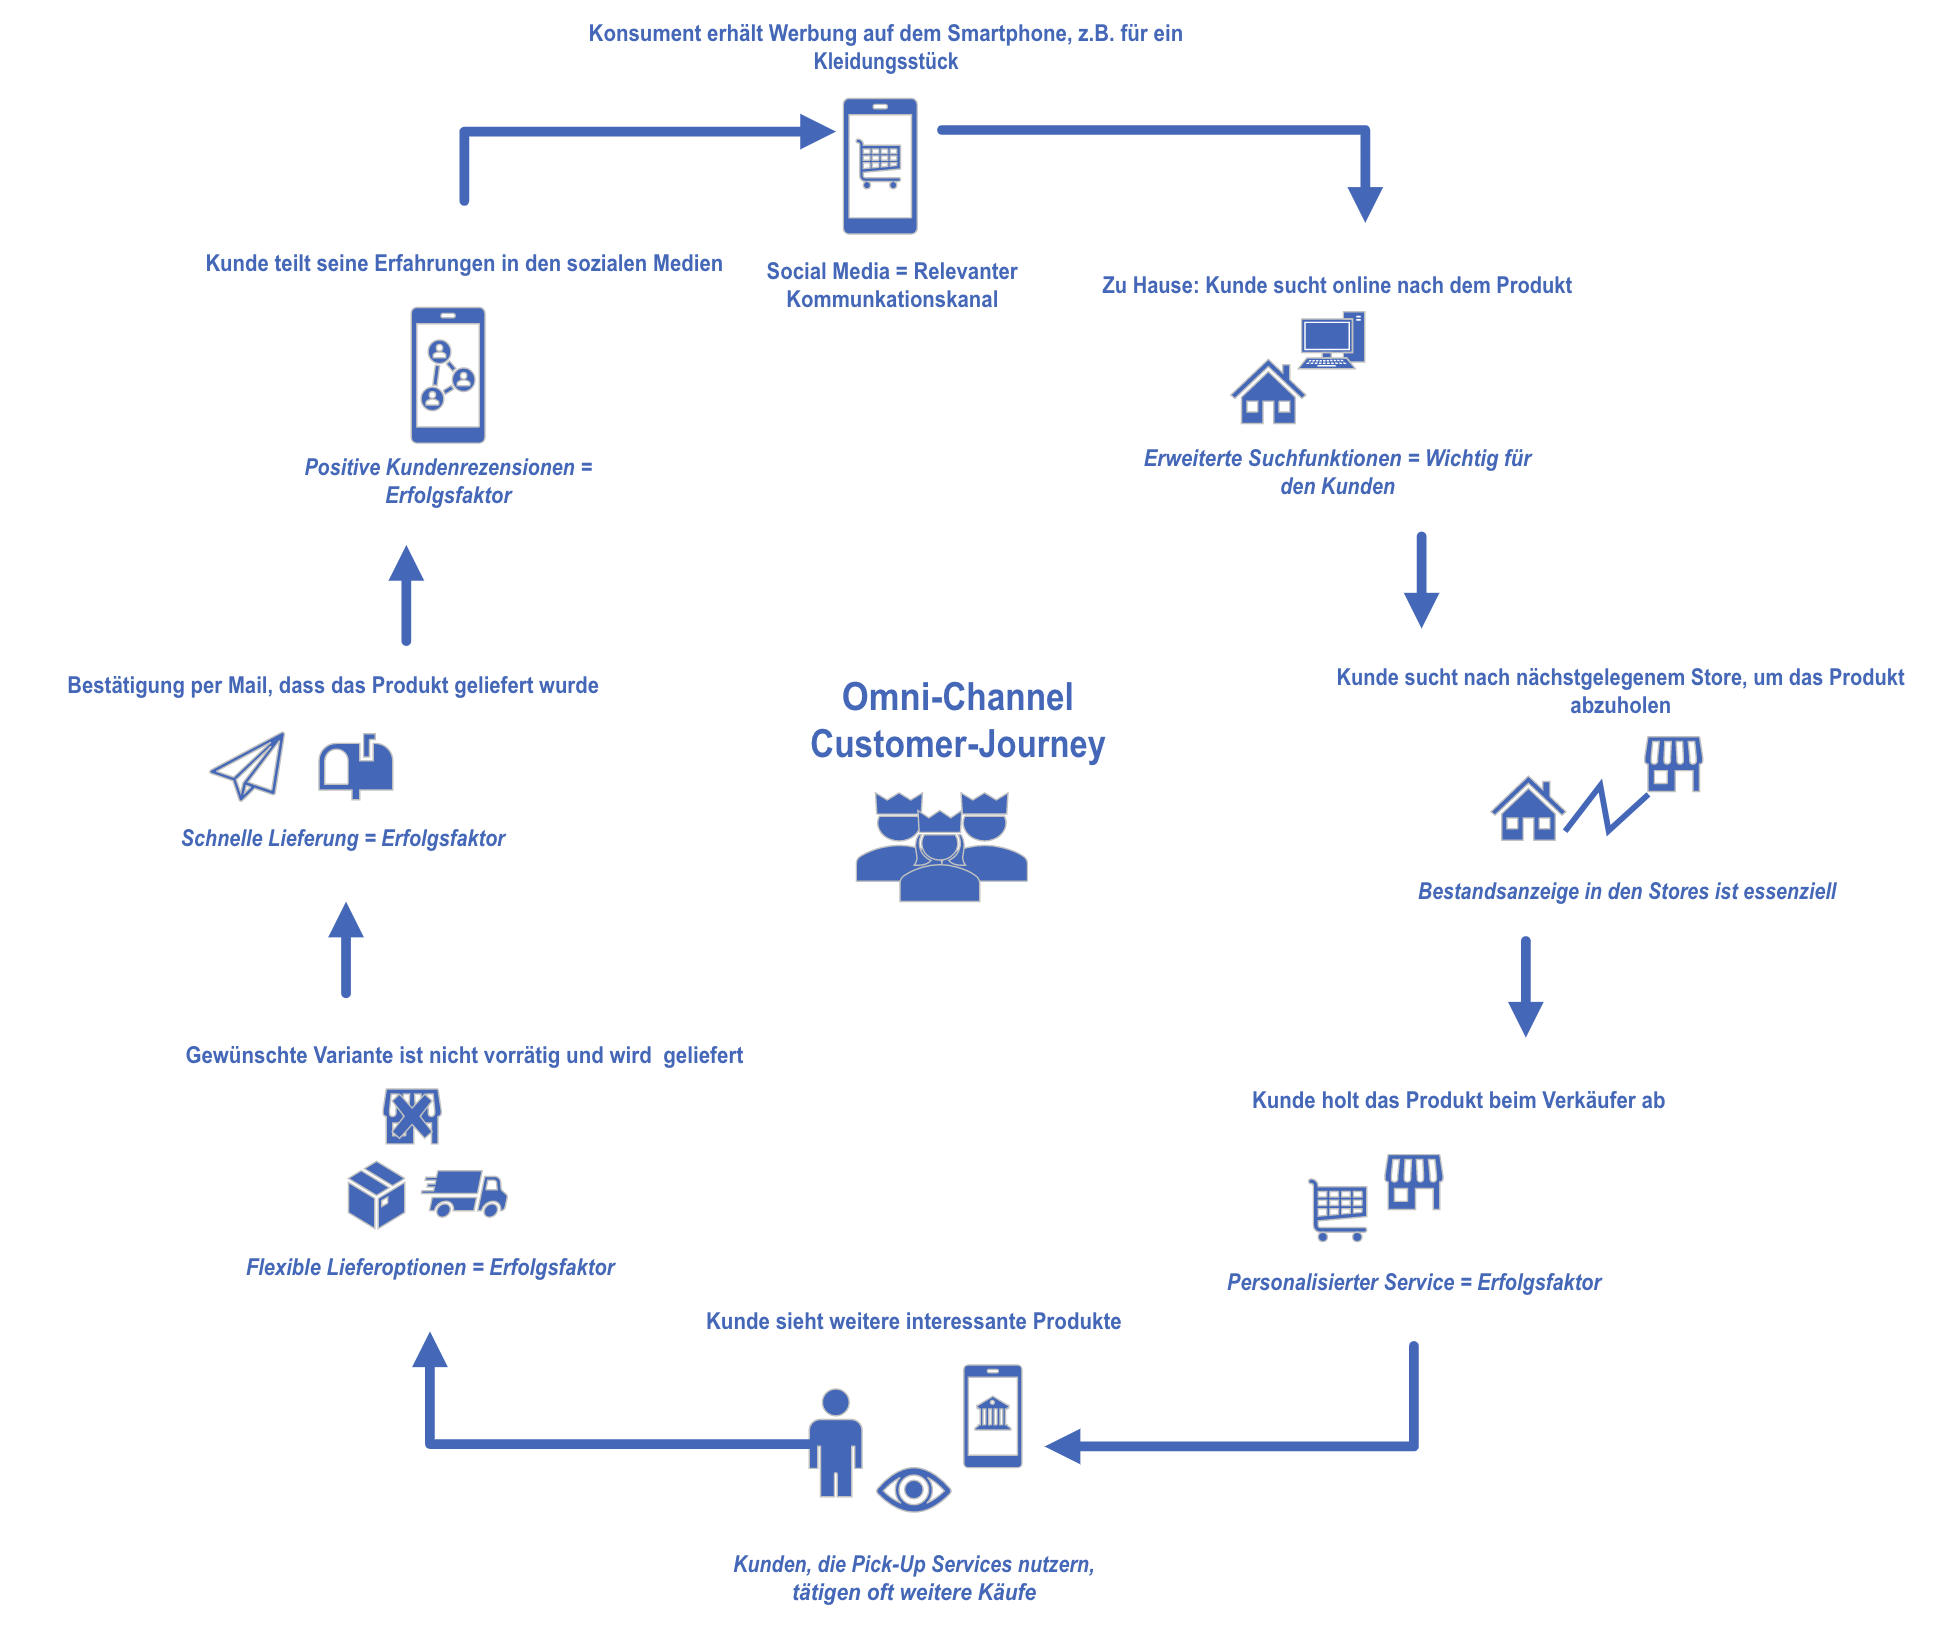
\includegraphics[width=0.95\textwidth,angle=0]{src/abbildungen/customer_journey.png}
    \caption[Quelle: Konzepte und Strategien für Omnichannel-Exzellenz S. 26, 2018]{Eine beispielhafte Customer Journey in Anlehnung an Böckenholt et all, Quelle: \autocite {Boeckenholt2018}}
   \label{customer_journey_2018}
   \end{figure}

\newpage
Die Customer Journey, also die Reise des Kunden oder Kundin, beschreibt den gesamten Prozess von der ersten Berührung, die der Kunde oder die Kundin mit dem Produkt widerfährt, bis hin zum Checkout, wo die Kaufabwicklung stattfindet.
\newline

Im Laufe der Customer Journey erreicht der Kunde oder die Kundin verschiedene Kontaktpunkte, sogenannte Digital Touchpoints. Durch die Auswertung der Digital Touchpoints können Informationen über den Kunden und Kundinnen gewonnen werden. Dieses Hintergrundwissen verbessert die Kundenberatung, die so proaktiv gestaltet werden kann. Durch die gewonnenen Informationen hat das Unternehmen die Möglichkeit, den Kunden oder die Kundin mit einer guten Beratung vom Produkt zu überzeugen\footnote{Vgl. \autocite [Online] {Duehning2021}}.
\newline

Im Normalfall entscheidet sich ein Kunde auch nicht direkt bei der ersten Berührung dafür, ein Produkt zu kaufen. Ein solcher Berührungspunkt in einem Einkaufsladen kann durch das Anschauen, das Sehen oder auch Riechen erfolgen. In der Regel gibt es zwischen Kunde und Produkt oder Marke mehrere Berührungspunkte, bis dieser überzeugt ist, das Produkt oder die Marke zu kaufen.
\newline

Eine Customer Journey von vor 10 Jahren ist jedoch nicht mehr mit einer Customer Journey von heute zu vergleichen, da sich die Einkaufsmöglichkeiten und die Verkaufskanäle im Laufe der Jahre durch die Digitalisierung verändert haben. Viele große Unternehmen haben bereits die Chance der technologischen Möglichkeiten ergriffen, den Kunden oder die Kundinnen einen nahtlosen Übergang der Verkaufskanäle anzubieten und die Customer Journey zu verbessern.
\newline

Dadurch, dass sich das Kaufverhalten enorm verändert hat und nicht mehr so linear verläuft, wie von dem AIDA-Modell dargestellt, entstanden einige neue Modelle, die eine Customer Journey beschreiben sollen. Als gemeinsamer Nenner wird bei diesen Modellen immer davon ausgegangen, dass die Kaufentscheidung ein Prozess ist, der nicht sofort getroffen wird. Dabei sollte berücksicht werden, dass durch die neuen Technologien (\ac{ua} KI) und Plattformen wie Social Media neue Phasen hinzu gestoßen sind.
\newline

Beim AIDA-Modell spielte der Prozess nach dem Kauf keine Rolle. Mundpropaganda und Meinungen über ein Produkt werden mittlerweile über Social Media Kanäle zum Beispiel von Blogger:innen und Influencer:innen heiß diskutiert und Bewertungen abgegeben.	 Nach dem Kauf kann man zwei Phasen ergänzend hinzufügen, wenn ein Unternehmen zum Beispiel bei einem Kunden oder einer Kundin nach dem Kauf nochmal explizit nach Feedback fragt und sichergeht, ob alles reibungslos bei der Lieferung abgelaufen ist und erfolgreich funktioniert. Wenn der Kunde mit dem Ablauf und dem Produkt zufrieden ist, führt dieses dazu, dass er in der Regel auch eher dazu tendiert, eine positive Bewertung für das Unternehmen abzugeben (Advocacy).
\newline

Ein Unternehmen, das die Customer Journey versteht, kann diese Kenntnisse nutzen, um gezielt im Marketing auf die Bedürfnisse und Präferenzen der Kunden einzugehen. Dies muss nicht zwangsläufig dazu führen, dass der Kunde das Produkt kauft, sondern kann dazu beitragen, verschiedene Ziele des Unternehmens zu erreichen, wie zum Beispiel das Abonnieren der Social-Media-Accounts, die Anmeldung für einen Newsletter, oder den Kauf eines anderen Produkts. Die Customer Journey bietet die Möglichkeit, die individuellen Ziele des Unternehmens zu verwirklichen\footnote{Vgl. \autocite [Online] {Gutmann2020}}.

\subsection{Customer Experience bei Omni-Channel-Strategien}\label{unterabschnitt_3_3}
Omni-Channel Kundenerfahrung (customer experience) bedeutet, dass ein Unternehmen Produkte und Kaufberatung über mehrere Kanäle an Interessenten und Kunden anbietet.
\newline
Jede Interaktion und jeder Berührungspunkt mit Kundenberater oder dem Produkt (soziale Medien, Chatbots, Kundenberatung) sind ein Teil dieser Customer Experience.
\newline

Der Omni-Channel-Ansatz ermöglicht es den Kunden und Kundinnen, die gesammelten Erfahrungen mit der Marke oder dem Produkt in einem Verkaufskanal zu beginnen und in einem anderen Kanal nahtlos fortzusetzen. Um dieses Ziel zu erreichen, müssen Unternehmen Ihre Marketing-, Vertriebs- und Kundensupport-Strategien aufeinander abstimmen.
\newline

Omni-Channel basierte Kundenerfahrungen (customer experience) sollten für Unternehmen kein Wunschtraum mehr sein. Für gut aufgestellte Unternehmen mit zukunftsorientiertem Denken ist es eine gute Chance, mit den neuen Technologien und Strategieansätzen die Verkaufskanäle noch stärker miteinander zu verknüpfen und neue Kunden-Features anzubieten. Mittel- und langfristig gesehen wird die Realität so aussehen, dass der Einsatz einer Omni-Channel-Strategie für Unternehmen mit mehreren Vertriebskanälen notwendig ist, um den modernen Verbraucher ansprechen zu wollen, da die Kundenbedürfnisse deutlich gestiegen sind und eine Customer Journey oft nicht mehr nur linear verläuft.
\newline

Das liegt daran, dass Verbraucher die Möglichkeit haben, eine ganze Reihe verschiedener Kanäle zu nutzen, um sich mit einer Marke oder einem Produkt auseinanderzusetzen und mehr zu erfahren. Beispiele sind die sozialen Medien, Videos, mobile Anwendungen oder die Google-Suche.
\newline

Omni-Channel-Kundenerlebnisse ermöglichen es Ihnen, den modernen Verbraucher an jedem Punkt seiner Reise zu erreichen, unabhängig davon, über welchen Kanal er zugreift. Dies wirkt sich positiv auf die Qualität der Kundeninteraktionen aus und führt zu einer stärkeren Kundenbindung. Die Einführung eines Omni-Channel-Ansatzes bringt sowohl für Kunden als auch für das Unternehmen eine Reihe von Vorteilen mit sich.
\newline

Sobald es zwischen den Konsumierenden und einem der Verkaufskanäle des Unternehmens die ersten Berührungspunkte gibt, erwartet der Konsumierende eine reibungslose Kundenerfahrung. Die Bereitstellung von unterschiedlichen Verkaufskanäle, die miteinander verknüpft sind und  mit denen der Konsumierende interagieren kann, hilft dabei, das Einkaufserlebnis so angenehm wie möglich zu gestalten, ohne dabei die Relevanz zu verlieren, dem Konsumierenden für das Produkt oder die Marke zu begeistern.
\newline

Mit Hilfe von Studien konnte gezeigt werden, dass die Kundenbindung und die Umsätze steigen, wenn mehrere Vertriebskanäle genutzt werden. Dabei haben Kunden und Kundinnen, die drei oder mehr Kanäle nutzen, um mit Marken zu interagieren, eine um 250 Prozent höhere Kaufhäufigkeit als Kunden, die nur einen Kanal nutzen. Die Harvard Business Review berichtet außerdem, dass Kunden, die mehr Kanäle nutzen, im Durchschnitt 4 Prozent mehr in Geschäften und 10 Prozent mehr online ausgeben.

\subsection{Äußere Einflussfaktoren}\label{unterabschnitt_3_4}
Äußere Einflussfaktoren müssen beim Omni-Channel-Retailing genauso berücksichtigt werden, wie die Anforderungen. Es handelt sich zwischen den Anforderungen und den äußeren Einflussfaktoren um ein Zusammenspiel, das sich in einem gegenseitigen Spannungsfeld befindet. Bei den äußeren Einflussfaktoren handelt es sich mit den Kundenanforderungen, Nachhaltigkeitsthemen und den technischen Entwicklungen um drei wichtige Faktoren, die für die Umsetzung einer Omni-Channel-Strategie berücksichtigt werden müssen\footnote{Vgl. \autocite [S. 26] {Vallee2018}}.
Durch die Nutzung neuer Technologien ist es möglich, dem Kunden oder der Kundin ein passendes Einkaufserlebnis zu verschaffen. Dafür wird im Verlauf dieses Abschnitts auf die technischen Prozesse eingegangen, die darstellen, wie ein solches Einkaufserlebnis personalisiert werden kann.

\subsubsection{Kundschaft im Zentrum}\label{unterabschnitt_3_4_1}
Beim Omni-Channel-Retailing spielen die Kundenanforderungen eine sehr wichtige Rolle. Diese Strategie zielt darauf ab, dem Kunden oder der Kundin ein nahtloses Einkaufserlebnis über alle Kanäle hinweg zu bieten. Dazu gehören sowohl Online- als auch Offline-Kanäle wie Filialen, Callcenter und Social Media.

\begin{figure}[!ht]
    \centering
    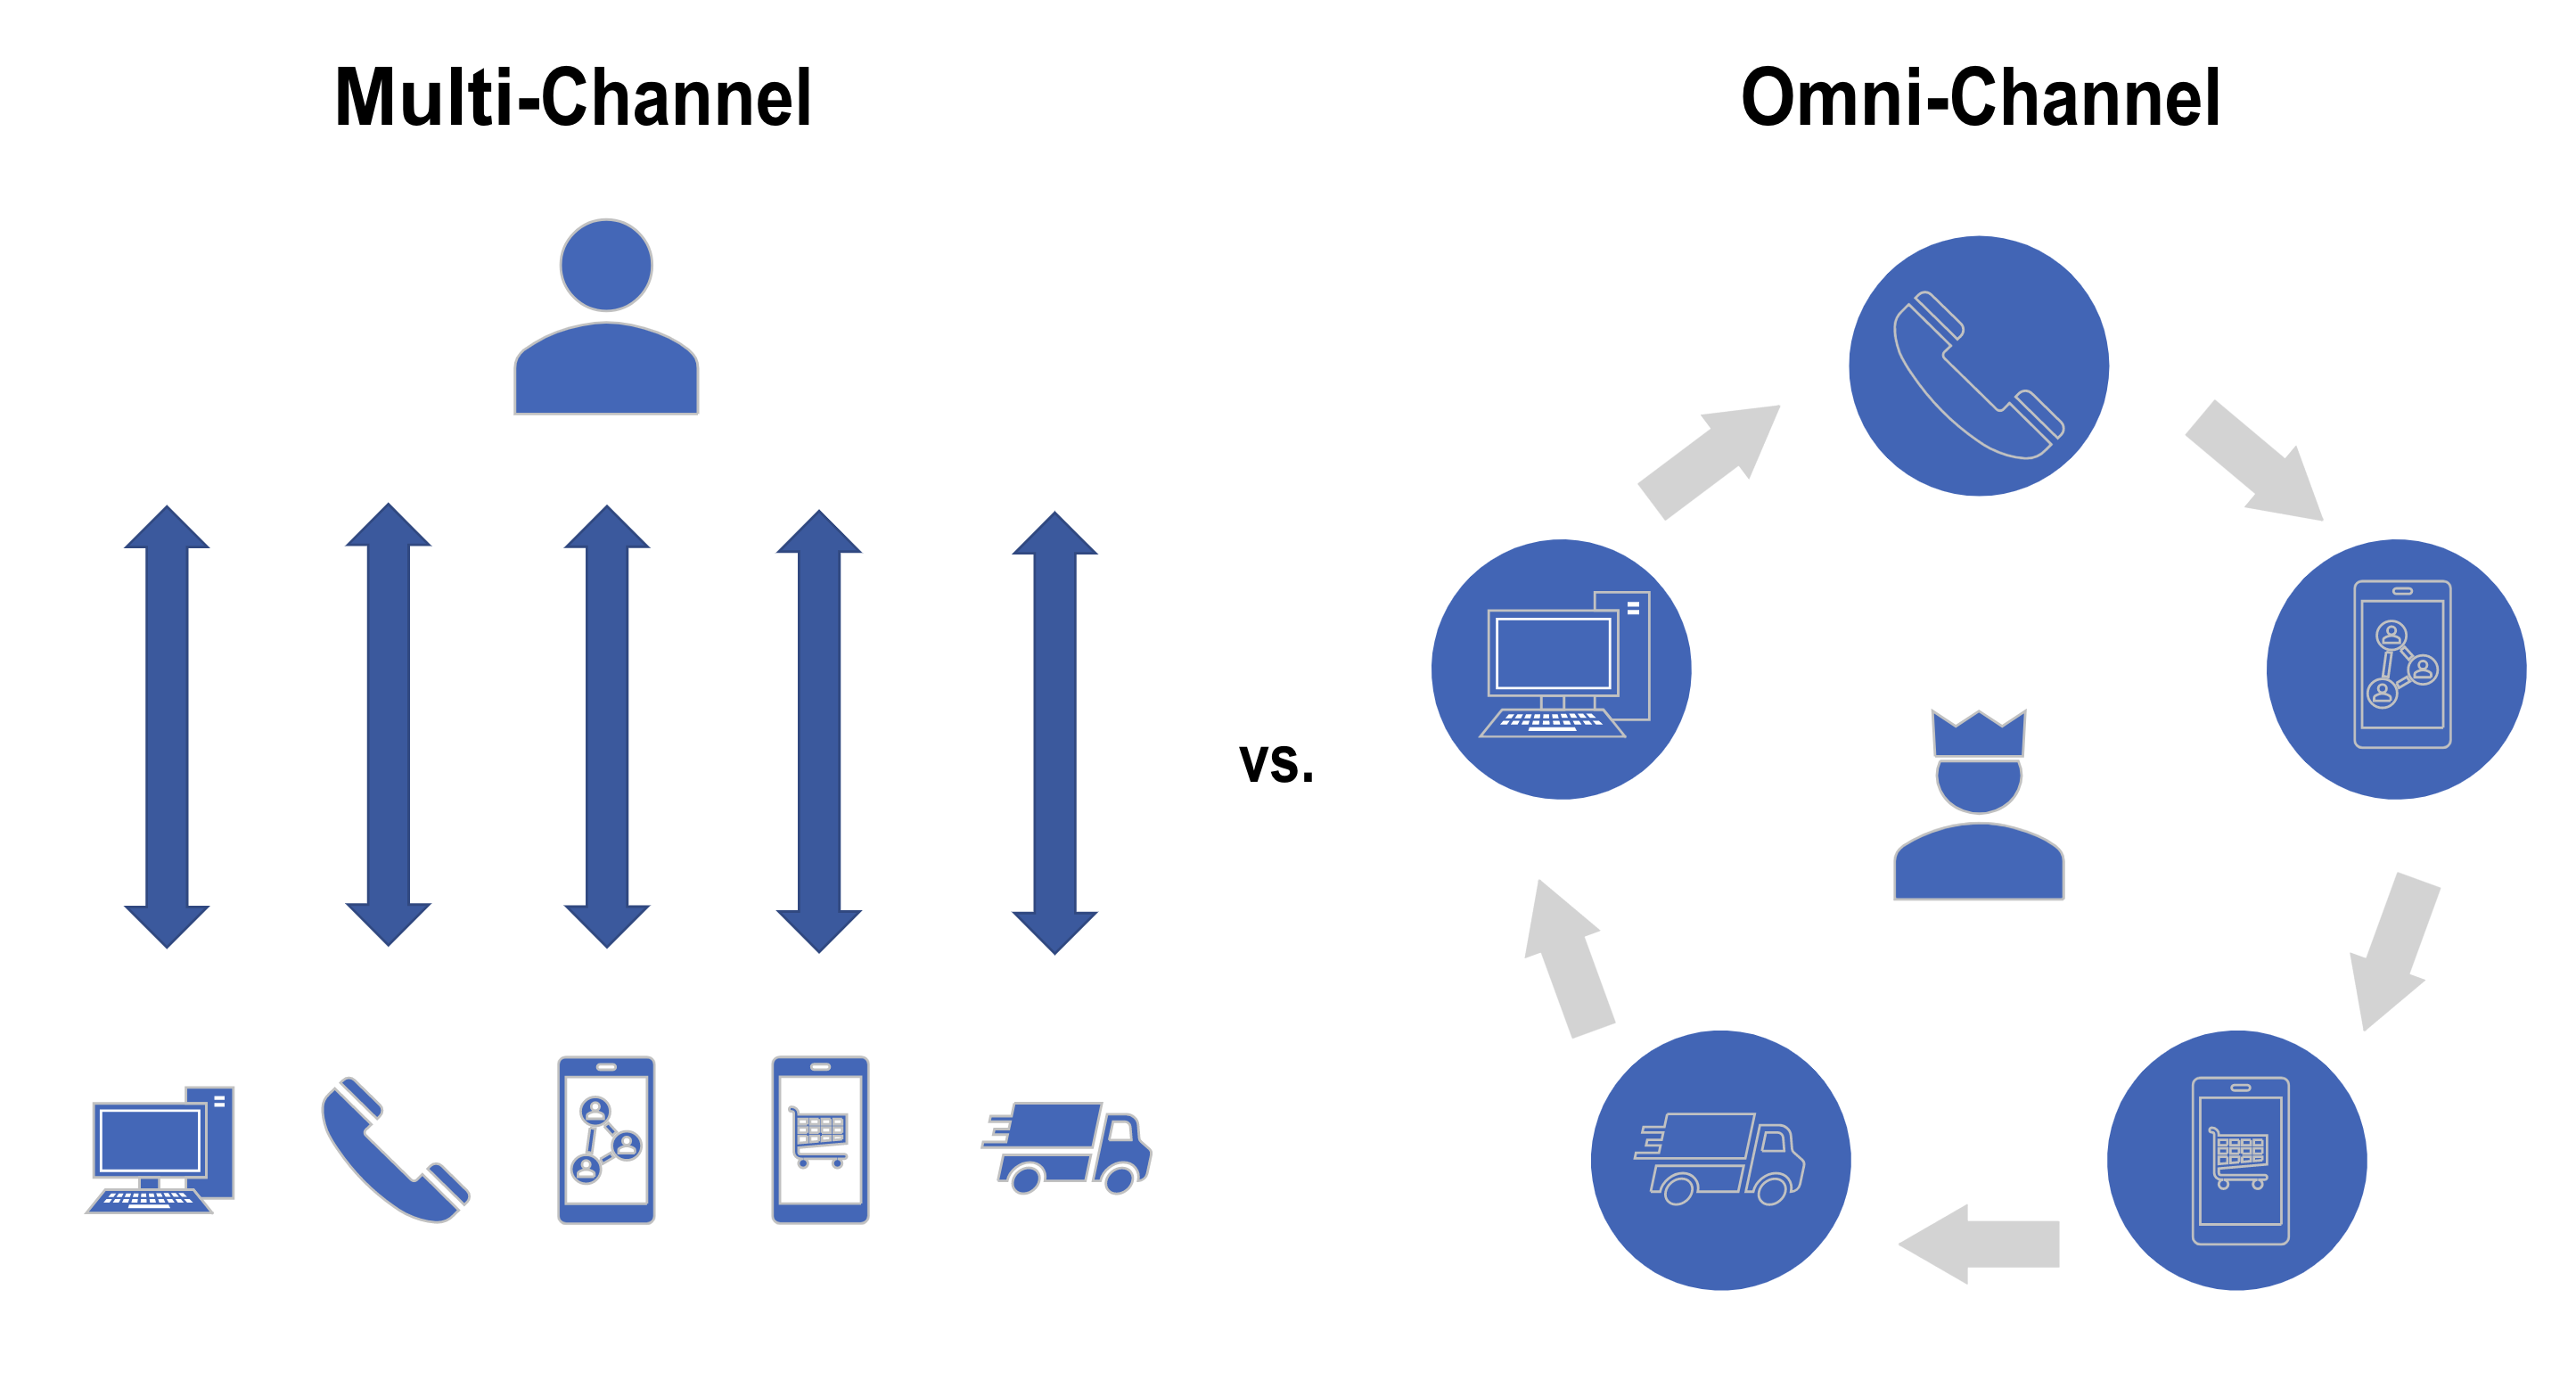
\includegraphics[width=1\textwidth,angle=0]{src/abbildungen/Multi-vs-Omni.png}
    \caption[Quelle: Omni-Channel Retailing S. 10, 2021]{Gegenüberstellung Multi-Channel-Marketing vs. Omni-Channel-Marketing in Anlehnung an Winters, Quelle: \autocite {Winters2021}}
   \label{fig: Quelle: omni_channel_retailing_2021}
   \end{figure}



Der Kunde oder die Kundin steht im Fokus der Omni-Channel-Strategie, da er oder sie auf allen verfügbaren Plattformen und in verschiedene Richtungen mit dem Unternehmen interagiert, um sich mit der Marke oder dem Produkt zu beschäftigen. Daher werden bei der Entwicklung einer Omni-Channel-Strategie die Bedürfnisse und Erwartungen der Kunden und Kundinnen sorgfältig analysiert und in den Prozess einbezogen. Ziel ist es, die bestmöglichen Angebote und Services bereitzustellen, die die Bedürfnisse der Kunden erfüllen und ihnen ein konsistentes und zufriedenstellendes Einkaufserlebnis bieten. Das bedeutet, dass ein Unternehmen die Präferenzen der Kunden in Bezug auf die Kanäle, die sie nutzen, um Produkte und Dienstleistungen zu erwerben und sich mit dem Unternehmen zu beschäftigen, berücksichtigen muss, um die bestmöglichen Ergebnisse zu erzielen. Es beinhaltet auch eine gute Kommunikation mit den Kunden und eine Möglichkeit für sie, ihre Erfahrungen und Bedürfnisse zu teilen, die wiederum für das Unternehmen wichtig sind, um sich weiter zu verbessern.
\newline

Eine erfolgreiche Omni-Channel-Strategie erfordert von Unternehmen die Schaffung von einem einheitlichen Kauferlebnis und einem konsistenten Erscheinungsbild. Damit eine solche Strategie erfolgreich umgesetzt werden kann, ist es wichtig, dass sowohl der Kunde als auch der Händler die volle Kontrolle über die Integration von Daten und Transaktionen haben, insbesondere in Bezug auf Preis, Lagerbestand, Lieferung und After-Sales-Service.
\newline
Bei dem Punkt Datenschutz treten jedoch vor allem im Internet große Probleme auf. Unternehmen müssen die Glaubwürdigkeit ihrer Kunden und Kundinnen gewinnen, damit diese sich auch bereit erklären, ihre Daten bereit zu stellen, so dass Unternehmen dann auch mit diesen Daten intelligent aufbereitet werden und für den Servicemitarbeiter zur Verfügung gestellt werden können.
Viele Konsumierende wären bereit, dem Unternehmen private Daten bereitzustellen. Das fehlende Vertrauen kommt jedoch daher, dass die Konsumierenden nicht wissen, was mit diesen Daten angestellt wird und die Konsumierenden am Ende des Tages nicht selbständig entscheiden können, was mit diesen Daten passiert. In diesem Fall muss der Prozess transparenter werden und die Konsumierenden müssen entscheiden können, was mit den Daten passieren darf.

Nach der Definition von Heinemann\footnote{Vgl. \autocite [S. 10] {Boeckenholt2018}} steht der Kunde oder die Kundin sogar vollständig im Fokus, wobei das Omni-Channel-Management nicht als Vertriebsstrategie, sondern als Verhaltensweise des Kunden betrachtet wird.
\newline

Kunden und Kundinnen nutzen heutzutage eine Vielzahl von Medien und Vertriebskanälen, weshalb sie ein konsistentes Kauferlebnis über alle Kanäle hinweg erwarten. Durch diese Entwicklung verschwinden die natürlichen Grenzen des Vertriebs und es ergeben sich für das Kundenbeziehungsmanagement neue Herausforderungen.
\newline

Eine wichtige Komponente einer erfolgreichen Omni-Channel-Strategie ist die Fähigkeit, die Präferenzen und Verhaltensweisen der Kunden und der Kundinnen zu verstehen und zu nutzen. Dies umfasst die Identifizierung von Mustern im Einkaufsverhalten, wie zum Beispiel welche Kanäle die Kunden am häufigsten nutzen, welche Art von Produkten oder Dienstleistungen sie am häufigsten kaufen und zu welchen Tageszeiten sie am aktivsten sind.
\newline

Basierend auf diesen Erkenntnissen kann ein Unternehmen die Angebote und Services an die Bedürfnisse der Kunden anpassen. Zum Beispiel, wenn die meisten Kunden und Kundinnen über Online-Kanäle einkaufen, kann ein Unternehmen seine Online-Präsenz verbessern, um diese Kunden besser zu bedienen. Wenn die meisten Kunden Produkte in einer Filiale kaufen, kann ein Unternehmen seine Filialen optimieren, um die Kundenerfahrung zu verbessern.
\newline

Eine Omni-Channel-Strategie erfordert auch die Fähigkeit, Daten über Kundeninteraktionen und Kundenaktivitäten über alle Kanäle hinweg zu sammeln und zu analysieren. Dadurch erhalten Unternehmen die Möglichkeit, ein vollständiges Kundenprofil zu erstellen und so ein personalisiertes Angebot und bessere Angebote und Dienstleistungen bereitzustellen. Omni-Channel-Retailing verbessert auch die Nutzung von Cross-Selling Angeboten, indem auf den Kunden zugeschnittene Angebote angeboten werden. Cross-Selling-Strategien sind in der Kosmetikbranche sehr verbreitet und es werden oft Produktlinien angeboten, die miteinander kombiniert werden können, um das bestmögliche Ergebnis zu erzielen. Beispielsweise kann ein Kosmetikunternehmen seinen Kunden, die eine Gesichtscreme kaufen, empfehlen, auch eine passende Augencreme oder eine Feuchtigkeitspflege zu erwerben. Durch ein personalisiertes Einkaufserlebnis kann zum Beispiel die eine bevorzugte Creme von der Lieblingsmarke des Kunden empfohlen werden.
\newline

Damit eine Omni-Channel-Strategie erfolgreich umgesetzt werden kann, muss das Unternehmen auch sicherstellen, dass alle Kanäle gut miteinander vernetzt sind und dass die Kunden nahtlos von einem Kanal zum anderen wechseln können. Dies bedeutet, dass Kundendaten und Kundeninformationen über alle Kanäle hinweg zentral gespeichert werden, um ein konsistentes und personalisiertes Einkaufserlebnis zu gewährleisten.

\subsubsection{Nachhaltigkeit mit Sicht auf die Kosmetikbranche}\label{unterabschnitt_3_4_2}
Heutzutage wird der Begriff Nachhaltigkeit in fast allen Branchen verwendet und hat in der Regel eine positive Konnotation. Dieser Begriff wird häufig mit ökologischem Wirtschaften, nachhaltiger Nutzung von Rohstoffen und umweltfreundlicher Produktion in Zusammenhang gebracht.
\newline

Aufgrund der Vielzahl verschiedener Anwendungsbereiche gibt es keine einheitliche Definition von Nachhaltigkeit. Es handelt sich um eine Reihe von Denkansätzen und Strategien, wie zum Beispiel "die Sicherung der menschlichen Existenz, die Erhaltung des gesellschaftlichen Produktivpotenzials und die Gewährleistung von Handlungs- und Entwicklungsmöglichkeiten für die heutigen und zukünftigen Generationen"\footnote{\autocite [S. 18] {Pufe2017}}.
\newline

Nachhaltigkeit ist in der Kosmetikbranche zu einem wichtigen Thema geworden. Immer mehr Menschen wollen sicher sein, dass die Produkte, die sie verwenden, nicht nur gut für ihre Haut, sondern auch für die Umwelt sind. Unabhängige Gütesiegel wie das BDIH-Prüfzeichen (Bundesverband deutscher Industrie- und Handelsunternehmen) gestalten den Kaufprozess transparenter und ermöglichen es dem Kunden nachzuvollziehen, ob ein Produkt nachhaltig produziert wurde\footnote{\autocite [Online] {Flatley2021}}.
\newline

Eine nachhaltige Kosmetikbranche ist eine, die umweltfreundliche und ethisch vertretbare Praktiken anwendet und sich verantwortungsbewusst gegenüber Menschen und Natur verhält. Dazu gehört zum Beispiel, dass Rohstoffe möglichst lokal und biologisch angebaut werden und der Einsatz von Mikroplastik vermieden wird.
\newline

Ein weiterer wichtiger Aspekt ist die Verpackung von Kosmetikprodukten. Es gibt mittlerweile viele Unternehmen, die auf umweltfreundliche Alternativen wie Glas oder Papier setzen, anstatt Plastikverpackungen zu verwenden. Es ist wichtig, dass möglichst jedes einzelne Unternehmen in der Kosmetikbranche ihren ökologischen Fußabdruck minimiert und gleichzeitig hochwertige, sichere und wirksame Produkte anbietet, um auch langfristig erfolgreich zu sein und einen wichtigen Beitrag zu einer nachhaltigen Zukunft leisten.
\newline

Tierversuche spielen für die Nachhaltigkeit in der Entwicklung von Kosmetikartikeln ebenfalls eine wichtige Rolle. Tierschutzorganisationen wie PETA haben viele Jahre dafür gekämpft, dass Tierversuche in der Kosmetikbranche verboten werden\footnote{\autocite [Online] {PETA2021}}.
Für einen Großteil der Kosmetikartikel ist das mittlerweile der Fall. Tierversuchsfreie Produkte werden von Unternehmen auch als Verkaufsargument genutzt, denn heutzutage fordert ein Großteil der Konsumierenden in der Kosmetikbranche Nachhaltigkeit bei Kosmetikprodukten. Eine repräsentative Studie der globalen Strategieberatung Simon-Kutcher \& Partners vom Januar 2022 hat gezeigt, dass 58\% der befragten Konsumierenden in der \acs{dach}-Region darauf Wert legen, dass Kosmetikartikel nachhaltig hergestellt wurden\footnote{\autocite [Online] {Simon2021}}. Mit nachhaltigen Produkten können sich Unternehmen nach außen besser und erfolgreicher vermarkten.
\newline

Das Kosmetik-Unternehmen BABOR setzt sich bereits seit Jahrzehnten das Ziel, nachhaltig zu Wirtschaften und bestehende Prozesse nachhaltig zu überprüfen, um noch bessere Alternativen zu entwickeln. Das Unternehmen legt dabei ein besonderes Augenmerk auf die Abwasserreinigung und Mülltrennung. BABOR stellt in regelmäßigen Abständen einen Plan, der über 5 Jahre zieht, auf und legt dabei fest definierte Ziele fest, die nachvollziehbar und ergebnisorientiert sind. Vor allem die Bereiche Verpackung und Zutaten sind ein sehr großes Thema, was die Produktion angeht. BABOR setzt und auch das Ziel, bis 2025 im Bereich des Green Packaging, der Verwendung von reinen Inhaltsstoffen und die Entstehung von CO²-Emissionen aktiv zu vermeiden, indem auf Öko-Erdgas, Photovoltaik Anlagen und Ökostrom gesetzt und klimaneutral gearbeitet wird, also weitestgehend auf Plastik verzichtet wird und Alternativen genutzt werden.  Auch der Bereich der Elektromobilität wird von BABOR gefördert\footnote{\autocite [Online] {BABOR2022}}.

\subsubsection{Technische Entwicklung}\label{unterabschnitt_3_4_3}

Welche technischen Prozesse werden bei einer Omni-Channel-Strategie angewendet? Was gibt es für Möglichkeiten und wie verläuft eine Kanalintegration?
\newline

Die Kundenanforderungen haben ein Level erreicht, in dem die Möglichkeit auf barrierefreies Einkaufen mit nahtlosem Wechsel zwischen den Verkaufskanälen und einer passenden Beratung zu den Produkten von vielen modernen Kunden gefordert wird. Unternehmen müssen versuchen, diesen Forderungen gerecht zu werden, um eine Marke oder ein Produkt langfristig erfolgreich vermarkten zu können.
\newline

Eine Grundvoraussetzung liefert ein zentrales Order Management System (OMS), das sämtliche Daten, die das Unternehmen betreffen, kanalübergreifend miteinander synchronisieren kann.

\begin{figure}[!ht]
    \centering
    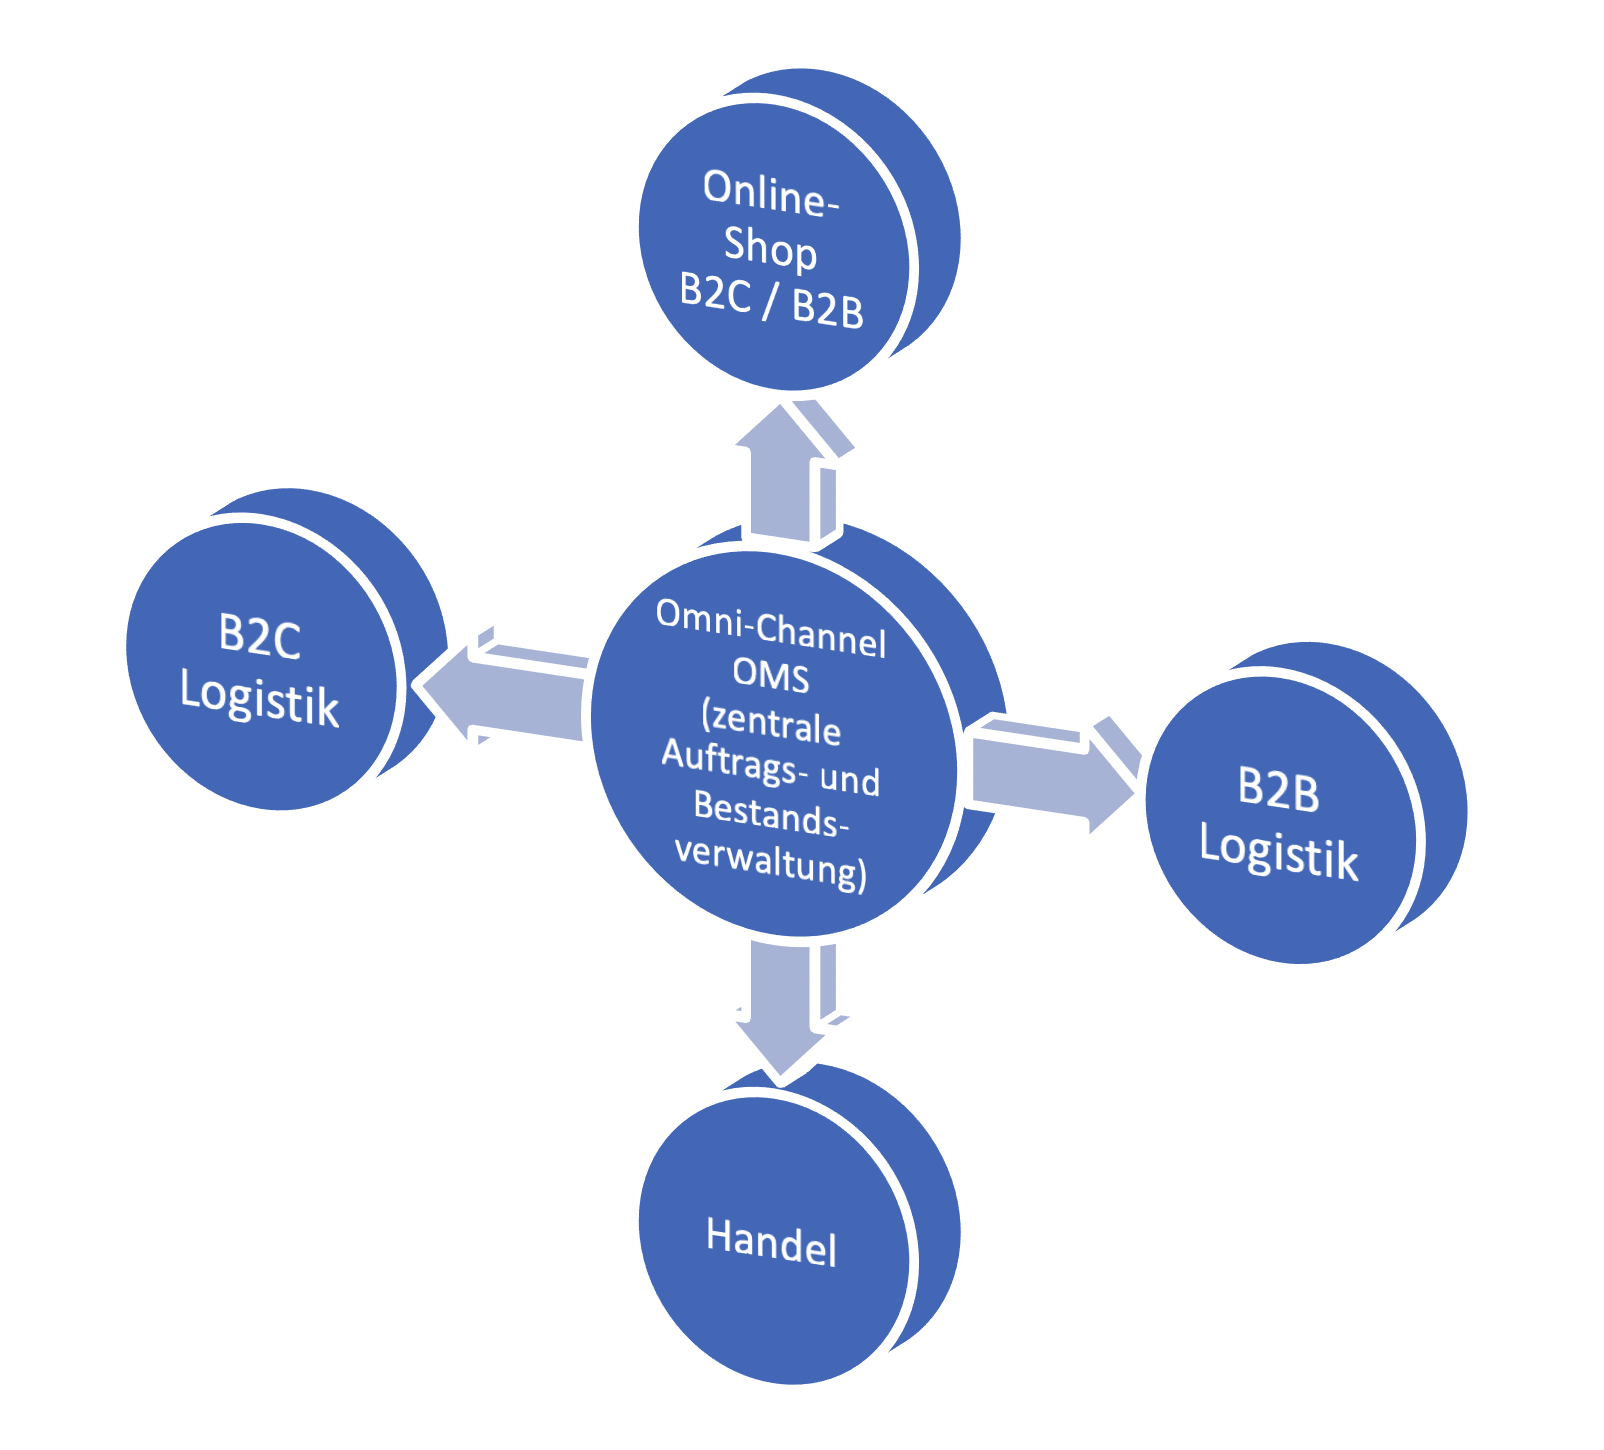
\includegraphics[width=1\textwidth,angle=0]{src/abbildungen/OMS-System.png}
    \caption[Quelle: Omni-Channel im Handel, 2018]{Zentrale Integrierung eines Order-Management-Systems in das Omni-Channel-Marketing in Anlehnung an Vallée et al, Quelle: \autocite {Vallee2018}}
   \label{fig: oms_system}
   \end{figure}

Dieses System bietet eine Schnittstelle für Verkaufskanäle, so dass diese ihre Daten miteinander synchronisieren können und Echtzeit Abfragen über aktuelle Bestände stattfinden können. Um die Möglichkeiten zu erweitern, kann das Kassensystem des Filialgeschäfts ebenfalls an das IT-System verknüpft werden, so dass kanalübergreifende Umsatzabfragen und Auswertungsmöglichkeiten bestehen.
\newline

Dort werden dann auch aufgezeichnete Daten mit Hilfe von Big Data Technologien gespeichert, die Informationen zu Kundengruppen oder auch einzelnen Kunden geben sollen. Big Data sind eine Vielzahl gesammelter Rohdaten, die Informationen über das Kauf- und Konsumverhalten von Konsumierenden liefern können. Diese Daten müssen verarbeitet werden, so dass Nutzdaten herausgefiltert und analysiert werden\footnote{\autocite [S. 6] {Fasel2016}}.
\newline

Mit Hilfe passender Software können Mitarbeiter die Informationen nutzen, um auf die Kundenbedürfnisse reagieren zu können und entsprechende Handlungsempfehlungen auszusprechen\footnote{\autocite [S. 28] {Vallee2018}}. Auch für den Bereich Marketing nimmt Big Data eine hilfreiche Rolle ein, indem zum Beispiel Auswertungen über Verkäufe über die Social-Media-Kanäle oder den Online-Shop getätigt werden können und Trends aufgezeigt werden.
\newline

Die Umsetzung für eine reibungslose und angenehme Auftragsabwicklung wird bei einem Omni-Channel-Retailing als Omni-Channel Fulfillment bezeichnet. Es kann vorkommen, dass einige Unternehmen für diesen Prozess oder bestimmte Teilaufgaben dieses Prozesses einen Logistikdienstleister beauftragen. Dazu gehören unter anderem die Produkte bzw. Waren, die kommissioniert, verpackt und an den Endkunden verschickt werden, aber auch die Abwicklung von Retouren.
\newline

Ein Unternehmen muss dabei abwägen, wie es strukturell aufgestellt ist, welche Kapazitäten zur Verfügung stehen oder wie groß die Lagerflächen sind. Daher kann es in bestimmten Fällen finanziell ein Vorteil sein, diese Aufgaben an einen Dienstleister abzugeben und sich so auf andere Kernpunkte wie den Service zu fokussieren. Weitere Teilprozesse, die das Omni-Channel-Fulfillment komplettieren, sind ein gut organisierter Check-Out-Prozess mit angenehmen Point-of-Sale Möglichkeiten und verschiedenen Lieferangeboten.
\newline

Gerade im Onlinebereich können dem Kunden über den POS eine Vielzahl von Optionen angeboten werden, um einen Kauf abzuschließen. Beispielsweise kann über ein geeignetes Shopsystem bei einer Onlinebestellung die Kaufabwicklung eines Stammkunden angenehmer gestaltet werden, indem die vorausgewählte Zahlungsart erkannt und automatisch hinterlegt ist oder passende Cross-Selling Angebote vorgeschlagen werden. Zudem erleichtert es dem Unternehmen, den Verkauf über mehrere Kanäle hinweg zu verfolgen und zu verwalten.
\newline

In der Kosmetikbranche nutzen bereits große Unternehmen die digitalen Möglichkeiten, um Kunden für sich zu gewinnen, indem sie ihre Produkte kanalübergreifend über ihren Online-Shop, einen Marketplace und in der Filiale verkaufen und gleichzeitig einen attraktiven Service anbieten. Dieser kann zum Beispiel Click \& Collect, Reserve \& Collect oder Return-to-Store Service sein. Bei dem Click \& Collect wird ein Einkauf online getätigt, beispielsweise über den Online-Shop und die Ware kann vor Ort in einer Filiale abgeholt werden\footnote{\autocite [S. 56] {Vallee2018}}.
Reserve \& Collect bietet dem Kunden die Möglichkeit, die Ware im Online-Shop zu reservieren und vor Ort am Point-of-Sale zu bezahlen und direkt mitzunehmen. Das Return-to-Store Angebot bietet dem Käufer bei einer Retoure die Möglichkeit, die online gekaufte Ware vor Ort in der Filiale umzutauschen.

\subsection{Potenziale und Herausforderungen des Omni-Channel}\label{unterabschnitt_3_5}
Die Digitalisierung hat nicht nur Auswirkungen auf den Handel. Durch die neuen Technologien entstehen tiefgreifende Veränderungen in der Denkweise der Gesellschaft. Deshalb müssen sich die Prozesse in Handelsunternehmen grundlegend anpassen und optimieren, um auf aktuelle und zukünftige Herausforderungen im Onlinehandel vorbereitet zu sein. Daraus können dann wiederum neue Türen geöffnet und neue Absatzgebiete erschlossen werden.
\newline

Die Vertriebsmöglichkeiten über den E-Commerce haben sich gefestigt und darüber hinaus sind sie mittlerweile in jedem großen Unternehmen ein fester Bestandteil der Unternehmensstruktur. Auch die Konsumierenden haben sich an die neuen Möglichkeiten gewöhnt und erwarten unter anderem permanente Verfügbarkeit der Online-Kanäle\footnote{\autocite [S. 426] {Heinemann2016}}.
\newline
Eine große Herausforderung stellt die Einrichtung der IT-Infrastruktur dar, die die verschiedenen Vertriebskanäle miteinander verschmelzen lassen und so einen nahtlosen Übergang der verschiedenen Kanäle garantieren soll.
Für die Anwendung einer Omni-Channel-Strategie ist eine zielgenaue Planung erforderlich. Daten über das Kaufverhalten der Kunden müssen gesammelt werden, um das Ziel, den Kunden in den Mittelpunkt zu stellen, erreichen zu können. Es gilt dabei herauszufinden, wie die Kunden ein Produkt kaufen wollen und welche Vertriebswege dabei für sie relevant sein können.
\newline

Bei der Planung werden Unternehmensstrukturen durchleuchtet und mögliche Anforderungsfälle erstellt. Zu einem solchen Prozess gehören nicht nur der Weg bis zum Warenkorb, sondern darüber hinaus auch Möglichkeiten, den Kunden zu unterstützen. Beispiele sind der Service, Vertrieb oder ein Produkt-Team.
\newline
Auch wenn das Live-System, auch Produktivsystem oder Produktivumgebung genannt, für die Verarbeitung der Software und den Quellcode des Online-Shops zuständig ist und damit das Herzstück für den Online-Shop darstellt, gibt es bei einer Omni-Channel-Strategie eine einzige Zentrale, die alle Verkaufskanäle miteinander verknüpfen soll. In den meisten Fällen nutzen Unternehmen dabei nicht den Online-Shop direkt, sondern eine \ac{erp}- und Warenwirtschafts-Lösung als Hauptquelle. Diese vereinfacht den Händlern unter anderem das Importieren und Migrieren von Produkten oder anderen Daten in den Online-Shop.
\newline
Die ERP- und Warenwirtschafts Lösung sorgt dafür, die betriebliche Effizienz zu verbessern, indem sie die Datenverwaltung zentralisiert, die Logistikprozesse optimiert und damit die Rentabilität erhöht und die Entscheidungsfindung erleichtert, indem sie mehr Transparenz bietet. In diesem Zusammenhang ist es genauso wichtig, die Schnittstellen so zu konfigurieren, dass die Datenintegrität reibungslos verlaufen kann und vollständig und korrekt konfiguriert wurde, um weitreichende Konsequenzen zu vermeiden, indem Informationen falsch weitergeleitet werden. Beispiele können Gutscheine oder Rabattaktionen sein, die kanalübergreifend funktionieren müssen, ohne Fehler zu produzieren. Das Controlling sollte dabei zentralisiert erfolgen.
\newline
Für neue Updates, Releases, aber auch mögliche Serverausfälle oder andere Infrastruktur-Ausfälle muss die Abteilung, die für die IT-Infrastruktur zuständig ist, möglichst präventiv oder schnell reagieren können, um Ausfallzeiten zu vermeiden und im besten Fall zu verhindern. Dieser Service für Wartung und das Entwickeln neuer Features oder Sicherheitsupdates für den E-Commerce Bereich wird in der Kalkulation für die Entwicklung eines Online-Shops bereits mit eingeplant. Bei der Verknüpfung der verschiedenen Verkaufskanäle wird der Umfang der Arbeit jedoch nicht geringer, es müssen noch mehr Prozesse berücksichtigt und eingebaut werden.
\newline

Dadurch lässt sich bereits erahnen, dass ein Unternehmen ein bestimmtes Budget investieren muss, um eine Omni-Channel-Strategie zu implementieren. Eine entscheidende Rolle spielt dabei auch die Größe des Unternehmens und wie viele Bestellungen in etwa pro Tag verschickt werden. Auch der Prozess beim Paketversand kann entsprechend optimiert werden.
\newline

Grundvoraussetzung für die Umsetzung einer Omni-Channel-Strategie ist für ein Unternehmen geeignetes Personal und Know How, um das Gerüst zu schaffen und eine Verkaufskanal übergreifende Infrastruktur aufzubauen. Zudem müssen alle Mitarbeiter geschult werden, um zu lernen, wie die Software funktioniert und genutzt werden kann.
\newline

Aus Käufersicht wird es ein wichtiger Punkt sein, den Point-of-Sale zum \ac{pop}, also dem Ort des Kaufs, umzugestalten. Entgegen dem POS agiert der POP nach dem Pull Prinzip. Dieses Prinzip wird als Pull-Prinzip bezeichnet, weil der Verkäufer keine Überzeugungsarbeit leisten muss, damit der Käufer ein Produkt aus Eigeninitiative aus dem Lager zieht. Der POP lässt sich auch im Online-Shop integrieren, indem zum Beispiel ein besonderes Produkt direkt auf der Hauptseite des Unternehmens besonders hervorstechen kann und so die Aufmerksamkeit des Konsumierenden auf sich ziehen kann.
\newline

Eine repräsentative Online Befragung von 2017 zeigte bereits einen Trend auf, dass obwohl die meisten deutschen Internetnutzer:innen den Einkauf im Geschäft bevorzugen, 70\% von ihnen mindestens einmal im Monat online einkaufen. Die Grenzen zwischen Online- und Offline-Käufen verschwimmen, da viele Käufer:innen ihr Smartphone nutzen, um sich über Produkte zu informieren und Coupons in Apps nutzen, um im Geschäft einzukaufen. Um die Konsumierenden effektiv anzusprechen, müssen Marken digitalen Content mit den stationären Einkaufserlebnissen verknüpfen\footnote{\autocite [Online] {Ipsos2017}}.
\newline

Gleichzeitig zeigt sich aber auch, dass Smartphones für Unternehmen eine wichtige Möglichkeit bieten, den Konsumierenden in einem entscheidenden Moment zum Kauf zu bewegen. Viele deutsche Online-Käufer:innen suchen bereits nach Produkten auf ihren Smartphones, nachdem sie Werbung gesehen haben, und mehr als die Hälfte der deutschen Onlinekäufer:innen kauften bereits 2017 über Apps auf ihrem Smartphone oder Tablet ein. Eine mobile Präsenz und Kommunikation ist daher ein wichtiger Faktor für Marken, um die Kundenbindung zu stärken und den Umsatz zu erhöhen. Personalisierte Push-Benachrichtigungen auf Basis der Daten der Benutzer:innen können die Aufmerksamkeit von Smartphone-Besitzern auf die Marke lenken, jedoch wird dieses Potenzial noch nicht ausreichend genutzt.
\subsection{Intralogistik}\label{unterabschnitt_3_6}
Die Intralogistik bezieht sich auf die innerbetrieblichen Prozesse der Materialwirtschaft und der Logistik. Im Zusammenhang mit dem Omni-Channel-Marketing in der Kosmetik-Branche schließt eine gut funktionierende Intralogistik dabei die Fähigkeit ein, Produkte und Bestellungen zwischen verschiedenen Vertriebskanälen, wie zum Beispiel Online-Shops, stationären Geschäften und Social-Media-Plattformen, zu verwalten und zu koordinieren.
\newline

Zur Intralogistik gehören Prozesse wie die Lagerhaltung, Kommissionierung, Verpackung und Versand. Eine effektive Intralogistik ermöglicht es Unternehmen auch, ihre Lagerbestände zu optimieren und dadurch Kosten zu sparen.
\newline

Um die Kundenbedürfnisse zu erfüllen und eine nahtlose Kundenerfahrung zu gewährleisten, besteht durch ein effizientes System für die Lagerverwaltung die Möglichkeit, die Lagerbestände zu optimieren und sicherzustellen, dass die Produkte zur richtigen Zeit am richtigen Ort verfügbar sind. Durch eine automatisierte Bestellabwicklung und -verarbeitung kann die Intralogistik sicherstellen, dass die Bestellungen schnell und präzise bearbeitet werden. Eine gut geplante Intralogistik ermöglicht es, die Versandprozesse zu optimieren und die Lieferzeiten zu minimieren. Die Rückverfolgbarkeit der Produkte ermöglicht es, eventuelle Probleme schnell zu erkennen und zu lösen. Mit Hilfe einer flexiblen Intralogistik kann auf Veränderungen bei der Nachfrage schnell reagiert werden und die Omni-Channel-Strategie entsprechend angepasst werden. Dabei muss berücksichtigt werden, dass eine effektive Intralogistik nur erreicht werden kann, indem die Prozesse in der gesamten Supply Chain betrachtet und optimiert werden.
\newline

In der Kosmetikbranche erfordert die Intralogistik oftmals auch besondere Anforderungen, wie z.B. die Einhaltung von Hygienestandards, Temperatur- und Feuchtigkeitskontrollen und die Verwendung von speziellen Lager- und Transportgeräten. Die Intralogistik ist ein wichtiger Erfolgsfaktor für die Umsetzung einer Omni-Channel-Strategie in der Kosmetikbranche sein.

\subsection{Faktoren für erfolgreiches Omni-Channel-Marketing}\label{unterabschnitt_3_7}
Wie bereits bei der Wichtigkeit der Customer Journey herauskristallisiert wurde, werden für eine erfolgreiche Umsetzung einer geeigneten Omni-Channel-Strategie zunächst die Kundenbedürfnisse analysiert, um die Strategie so anzupassen, dass der Kunde bei seinem Einkaufserlebnis ein Gefühl vermittelt bekommt, bei dem der Einkauf für ihn reibungslos verläuft und Spaß macht.
\newline

Ein wichtiger Erfolgsfaktor um eine Omni-Channel-Strategie erfolgreich umzusetzen ist, dass die Marketingstrategien kanalübergreifend synchronisiert werden, um eine nahtlose und personalisierte Kundenerfahrung zu ermöglichen. Dafür können wichtige Faktoren berücksichtigt werden. Voraussetzung für die Synchronisierung ist ein geeignetes und zentralisiertes ERP-System, an dem sämtliche Produktinformationen angeschlossen sind. Das zentral geführte System muss also auch den hohen Anforderungen gerecht werden, um sämtliche Daten verarbeiten zu können, die über alle Vertriebskanäle hinweg gehen. Bei der Suche nach geeigneter Software macht es Sinn, nach dem Best-of-Breed-Ansatz zu handeln. Dies bedeutet, dass für jedes Verwaltungssystem die bestmögliche spezialisierte Lösung ausgewählt wird, anstatt eine allgemeine Lösung zu verwenden.
\newline

Beispielsweise kann ein Unternehmen, das den Best of Breed-Ansatz verfolgt, für seine Finanzbuchhaltung eine spezialisierte Software verwenden, für seine Kundenbeziehungsverwaltung (CRM) eine andere spezialisierte Software und für seine Personalverwaltung eine weitere spezialisierte Software. Diese spezialisierten Lösungen können dann miteinander integriert werden, um eine umfassende Unternehmenslösung zu erhalten\footnote{\autocite [Online] {Woromsbecher2021}}.
\newline

Ein CRM-System stellt das Herzstück von bei einer Omni-Channel dar, weil es Unternehmen dabei unterstützt, eine nahtlose, konsistente und personalisierte Kundenkommunikation über verschiedene Kanäle hinweg zu gewährleisten. Ein CRM-System ermöglicht es Unternehmen, alle Kundeninteraktionen zentral zu erfassen und zu speichern, unabhängig davon, über welchen Kanal (z.B. E-Mail, Telefon, soziale Medien) die Interaktion stattfindet. Durch die Verknüpfung dieser Interaktionen innerhalb des CRM-Systems kann ein Unternehmen einen umfassenden Überblick über das Verhalten und die Bedürfnisse eines Kunden oder einer Kundin gewinnen und somit eine personalisierte und konsistente Kommunikation über alle Kanäle hinweg gewährleisten.
\newline
Darüber hinaus ermöglicht ein CRM-System Unternehmen, Kundenprofile zu erstellen, die Informationen wie Kaufhistorie, Präferenzen, Feedback und Support-Anfragen enthalten. Diese Profile können dann genutzt werden, um personalisierte Marketingbotschaften, Empfehlungen und Angebote an den Kunden zu senden, unabhängig davon, über welchen Kanal er mit dem Unternehmen interagiert.
\newline
Ein weiterer Vorteil von CRM-Systemen im Omnichannel-Kontext ist die Möglichkeit, Daten aus verschiedenen Quellen wie Vertrieb, Marketing, Kundenservice und E-Commerce zu integrieren. Dies ermöglicht es Unternehmen, ein umfassendes Verständnis für den Kunden zu entwickeln und eine konsistente Erfahrung über alle Kanäle hinweg zu bieten.
\newline

Um die Kunden und Kundinnen zu erreichen, sollten Unternehmen personalisierte Angebote machen, die auf den individuellen Bedürfnissen und Wünschen der Kunden und Kundinnen basieren. Dies kann beispielsweise durch die Verwendung von Datenanalyse erreicht werden, um die Präferenzen der Kunden zu erkennen und personalisierte Angebote zu erstellen. Dazu gehören dann unter anderem auch Rabattaktionen oder Aktionstage wie der Black Friday, an denen es besondere Angebote gibt.
\newline

Für die Synchronisierung ist es auch wichtig, eine einheitliche Marke über alle Kanäle hinweg zu entwickeln. Dies bedeutet, dass das Branding und die visuelle Identität auf allen Kanälen konsistent sein sollten, um eine starke und erkennbare Marke zu schaffen. Dazu gehören zum Beispiel auch ein geeignetes Logo und markante Farben, die die Identität des Unternehmens widerspiegeln.
\newline

In der heutigen digitalen Welt ist die Nutzung von Social-Media ein wichtiger Bestandteil des Omni-Channel-Marketings. Besonders in der Kosmetikbranche sollten Unternehmen ihre Präsenz auf verschiedenen Social-Media-Plattformen aufbauen und pflegen, um eine breite Zielgruppe zu erreichen und Interaktionen mit Kunden zu fördern. Ein weiterer wichtiger Faktor ist die mobile Optimierung, gerade weil immer mehr Menschen über mobile Geräte auf das Internet zugreifen. Unternehmen sollten sicherstellen, dass ihre Websites und Online-Shops für mobile Geräte optimiert sind, um eine reibungslose Benutzererfahrung zu gewährleisten. Zudem ist auch ein guter Kundenservice unerlässlich für erfolgreiches Omni-Channel-Marketing. Unternehmen sollten sicherstellen, dass sie über mehrere Kanäle erreichbar sind und dass ihre Mitarbeiter gut geschult und in der Lage sind, Fragen und Probleme schnell und effektiv zu lösen.
\newline

Um die Grundvoraussetzung zu schaffen, Omni-Channel-ready zu sein, wird ein geeignetes Shopsystem empfohlen, auf dem der Online-Shop aufgesetzt wird. Für die Produkte sind zum Beispiel passende Filtermöglichkeiten und ein einfach abgebildeter Checkout-Prozess beim Online-Einkaufserlebnis integriert. Die Shopsysteme bieten viele verschiedene Erweiterungen direkt an, die kostenlos sind oder für einen Aufpreis dazu gebucht werden können. Es ist jedoch auch möglich, Erweiterungen, die den Anforderungen entsprechen, selbst zu entwickeln. Ein Beispiel können personalisierte Cross-Selling Angebote sein, den Kunden dazu animieren, passende Partnerartikel zum Warenkorb hinzuzufügen.
\newline

Zudem bieten viele Shopsysteme wie Shopware oder Magento den Vorteil, den Headless Commerce Ansatz zu verfolgen. Headless Commerce ist ein Ansatz für den E-Commerce, bei dem die Frontend- und Backend-Systeme voneinander getrennt sind. Das Backend, das für die Verwaltung von Produkten, Bestellungen und Kunden verantwortlich ist, wird von einem Frontend, das für die Anzeige der Produkte und die Interaktion mit dem Kunden verantwortlich ist, getrennt. Headless Commerce gewinnt bei Unternehmen immer mehr an Beliebtheit, weil es viele Vorteile bietet. Zum einen ermöglicht es durch die unabhängige Entwicklung zwischen den Frontend- und Backend-Systemen eine größere Flexibilität bei der Gestaltung der Benutzeroberfläche. Zum anderen wird ermöglicht, dass das Frontend auf verschiedenen Plattformen wie Web, Mobile, und Sprachassistenten angeboten werden kann. Zusätzlich wird die Skalierbarkeit und Leistung der Systeme erhöht, da die Last zwischen den Frontend- und Backend-Systemen aufgeteilt wird.
\newline

Zudem bieten Headless-Shopsysteme Händlern die Möglichkeit, den Online-Shop stetig weiterzuentwickeln, neue Vertriebskanäle schnell zu integrieren und den Kunden eine optimale Customer Experience zu bieten. Dies ist bei Omni-Channel Strategien von großer Bedeutung, da technologische Entwicklungen schnell dazu führen können, dass das, was heute als Standard gilt, morgen bereits veraltet ist. Langfristige Flexibilität ist für Händler deshalb ein wichtiger Faktor\footnote{Vgl. \autocite [S. 89] {Boeckenholt2018}}.
\newline

Aus der repräsentativen Studie “Shopper Story 2020” von der E-Commerce Agentur Criteo können in Bezug auf Omni-Channel-Strategien interessante Blickwinkel geschlossen werden. Dabei wurden Konsumierende unterschiedlicher Generationen unter anderem befragt, worauf bei einem Einkauf Wert gelegt wird und welche Verkaufskanäle am beliebtesten sind.
\newline

Etwas mehr als jeder zweite Deutsche der Generation Z (geboren in den letzten 28 Jahren bis 1994) und der Millennials (geboren zwischen 1981 und 1994) würden im stationären Laden einkaufen, wenn sie die Zeit dazu haben. Um neue Trends kennenzulernen oder Informationen zu erhalten, würde nur jede dritte Person der jüngeren Generationen einen stationären Handel aufsuchen. Wenn es die Zeit zulässt, würden bei der Generation X (geboren zwischen 1965 und 1980) und älter hingegen bereits knapp 70\% der Konsumierenden den stationären Handel besuchen. Dadurch, dass die jüngeren Generationen mit dem Wandel der Digitalisierung aufgewachsen sind, ist das Verständnis in diesem Kontext bei ihnen deutlich größer als bei den älteren Generationen. Dementsprechend ist die Abhängigkeit zum stationären Handel nicht so ausgeprägt wie bei den anderen Generationen.
\newline

Auch für die Kosmetikprodukte lassen sich Rückschlüsse ziehen. Zeit ist für viele Menschen ein wichtiger Faktor geworden und am Umsatz des Online-Handels zeigt sich, dass das Online-Shopping auch in der Kosmetikbranche immer wichtiger wird.
\newline

Ein Unternehmen sollte Aktionstage wie den Black Friday einbauen, um neue Kunden auf sich aufmerksam zu machen, denn Rabattaktionen sind sehr beliebt. Im Durchschnitt nutzen zwei von drei Konsumierenden Rabatt Gutscheine und Aktionen für den Kauf von Produkten. Rabatt-Codes motivieren die jüngeren Generationen in über 55\% der Fälle erst dazu, ein Produkt zu kaufen. Während es bei den älteren Generationen 44\% sind.
\newline

Wenn ein Unternehmen den Kundenbedürfnissen gerecht werden kann, führt dies dazu, dass über gute Rezensionen und Mundpropaganda neue Kunden angelockt werden. Jeder zweite Käufer, der eine gute Einkaufserfahrung sammelt, bewertet das Unternehmen positiv.
\newline

Nicht nur in Zukunft, sondern bereits auch heute schon nutzen besonders die jungen Generationen Apps, um Produkte anzuschauen, sich inspirieren zu lassen, Bewertungen zu vergleichen, Produkte zu kaufen oder auch den Bestellstatus zu überprüfen. Mit Blick auf die Zukunft wird prognostiziert, dass die Wichtigkeit von Apps nochmal deutlich ansteigen wird.
Die Mehrheit der Konsumierenden nutzen unbewusst bereits Omni-Channel-Ansätze, indem sie sich online über Produkte informieren und diese dann in der Filiale kaufen oder das Produkt online gekauft wird, nachdem es in der Filiale zuvor angeschaut wurde.
\newline

Für die Verbesserung der Kundenbedürfnisse können viele verschiedene Erlebnismöglichkeiten bei einer Customer Journey integriert werden. Daher ist es wichtig, dass die Online- und Offline Kanäle konsistent ineinander verlaufen und der Online-Shop die Identität des Unternehmens widerspiegelt.

\subsection{Die letzte Meile}\label{unterabschnitt_3_8}
Die letzte Meile spielt eine entscheidende Rolle in Omni-Channel-Strategien, da sie den letzten Schritt des Kaufprozesses darstellt und somit einen wichtigen Einfluss auf die Kundenbindung und -zufriedenheit hat. Sie bezieht sich dabei auf den Lieferprozess von Produkten oder Dienstleistungen zum Kunden. Dazu gehören die Lieferung, die Lieferzeiten und die Lieferoptionen. Unternehmen, die eine erfolgreiche Omni-Channel-Strategie verfolgen, achten daher darauf, dass die letzte Meile so reibungslos und zufriedenstellend wie möglich gestaltet wird, indem sie zum Beispiel flexible Lieferoptionen anbieten, Lieferzeiten transparent kommunizieren und den Kunden über den Lieferstatus auf dem Laufenden halten. Eine effiziente Logistik ist entscheidend, um eine zuverlässige und schnelle Lieferung zu gewährleisten und die Anzahl der Bestellungen möglichst schnell und erfolgreich abzuwickeln. Für die Nachverfolgung muss eine robuste Technologie zur Verfügung stehen, die einen Überblick über den Lieferstatus bietet.
\newline

Es müssen zudem angemessene Lieferkosten berechnet werden, die den Kunden und die Kundin nicht abschrecken, aber auch die Kosten für das Unternehmen decken. Viele Unternehmen bieten einem erreichten Mindestbestellwert eine versandkostenfreie Lieferung an. Diese Strategie animiert den Kunden in einigen Fällen dazu, ein weiteres Produkt hinzuzufügen, um eine versandkostenfreie Bestellung zu ermöglichen. Auch wenn in diesem Fall das Unternehmen die Versandkosten übernimmt,  sorgt die Gewinnmarge dafür, dass die Bestellung für das Unternehmen trotzdem erfolgreich ist. Mit nachhaltigen Liefermethoden, die den Umwelteinfluss minimieren, kann das Image des Unternehmens verbessert und die Kundenbindung gestärkt werden. Nachhaltige Liefermethoden können zum Beispiel sein, wenn über Click \& Collect online bestellt wird und das Produkt an die Filiale geliefert wird. So wird es dem Unternehmen ermöglicht, die Lieferung mit anderen Produkten, die an die Filiale gesendet werden, zu verbinden.
\newline

Auch der Punkt Datenschutz spielt eine wichtige Rolle. Der Schutz sensibler Kundendaten, wie Adressen und Kreditkartendetails, ist wichtig, um das Vertrauen der Kunden zu gewinnen und Sicherheitsbedenken zu vermeiden.
\newline

Eine gut gestaltete letzte Meile trägt dazu bei, die Kundenbindung zu stärken und die Wahrscheinlichkeit zu erhöhen, dass der Kunde und die Kundin erneut beim Unternehmen einkaufen.
Eine Studie des Bundesverbandes Paket und Expresslogistik von 2022 verdeutlicht das Wachstum, das der E-Commerce im letzten Jahrzehnt verzeichnet hat\footnote{Vgl. \autocite [Online] {Bundesverband2021}}.
\newline

Durch die vielen Online-Bestellungen, die im Laufe der letzten 10 Jahre stetig anstiegen, wurden 2011 noch 2,47 Milliarden Pakete pro Jahr über \ac{kep}-Dienstleister (Kurier-, Express- und Paketsendungen), wie \ac{dhl}, \ac{dpd}, Hermes, \ac{ups} oder \ac{gls} verschickt. Im Jahr 2021 wurde gegenüber 2011 bereits ein Anstieg von über 82\% erreicht und über 4,5 Milliarden Pakete verschickt.
\newline

Das stärkste Wachstum verzeichnete hierbei der B2C-Bereich mit einem Anstieg von 16,6\% zum Vorjahr 2020. Verantwortlich dafür ist zum Großteil das dynamische Wachstum des Online-Handels, dass den B2C-Bereich damit zum stärksten Treiber bei den KEP-Dienstleister macht. Der B2B-Bereich musste 2021 hingegen einen Rückschritt um -1,5\% zum Vorjahr 2020 vollziehen, da es oftmals zu bekannten Schwierigkeiten in der Lieferkette und damit verbundenen Produktionseinschränkungen kam.
\newpage
\section{Umsetzung einer Omni-Channel-Strategie bei BABOR}\label{hauptabschnitt_4}

\subsection{Das Unternehmen BABOR}\label{unterabschnitt_4_1}

Die Geschichte des Unternehmens BABOR begann 1956 mit der erfolgreichen Entwicklung einer Rezeptur von dem Chemiker Dr. Michael Babor für das Reinigungsöl HY-ÖL, das bis heute als Verkaufsschlager und Kernprodukt von BABOR auf sämtlichen Plattformen verkauft wird. Das Kosmetik Start-Up wurde im selben Jahr von dem Pharmazeuten Dr. Leo Vossen aufgekauft und gilt seitdem als Familienunternehmen in mittlerweile dritter Generation.
\newline

BABOR ist ein 65 Jahre altes deutsches Kosmetikunternehmen, das Produkte zur Hautpflege im Luxussegment in über 70 Ländern verkauft. Das Lager, die Entwicklung und die Produktion für die eigens entwickelten Produkte finden in Deutschland in der Stadt Aachen statt. Die Marke BABOR umfasst jedoch nicht nur das Reinigungsöl HY-ÖL, sondern auch weitere Produkte im Bereich der Hautpflege. BABOR vermarktet Produkte für Gesichtspflege, Körperpflege, Hand- und Fußpflege, organische Hautpflege, Männerpflege, Sonnenpflege, dekorative Kosmetikprodukte und Düfte.
\newline

BABOR hat sich seit seiner Gründung zu einem Marktführer für professionelle Kosmetik entwickelt. BABOR nutzt vor allem Zutaten aus der Umgebung für die Herstellung ihrer Cremes, Lotionen und Ampullen. Nach eigenen Angaben hat das Unternehmen 2021 insgesamt rund 200 Millionen Euro umgesetzt\footnote{ Vgl. \autocite [online] {Finance2021}}.
\newline

BABOR ist in Deutschland in über 2000 Kosmetikstudios vertreten. Zudem verkaufte BABOR seine Produkte lange Zeit hauptsächlich über den B2B Bereich und pflegt in diesem Bereich viele intensive Kundenbeziehungen mit großen Unternehmen oder Beauty Ketten wie Douglas und Flaconi, wo die Produkte dann schlussendlich in den Regalen stehen und an den Endkunden weiterverkauft werden sollen. Seit 2014 hat BABOR die Unternehmensphilosophie hin zu dem Angebot über mehrere Verkaufskanäle verändert.

\subsection{Forcierung des Onlinegeschäfts}\label{unterabschnitt_4_2}
Durch die Übernahme der dritten Familiengeneration im Management wurde 2016 mit dem früheren L'Oreal Manager Tim Waller zusätzlich auch ein neuer CO-Geschäftsführer eingestellt. Dabei wurde das Ziel gesetzt, mittel- und langfristig auch vermehrt in das Online-Geschäft zu investieren.
\newline

Dafür wurde zunächst zwar hauptsächlich der europäische Markt angepeilt, es wurden aber auch Kooperationen mit ausgewählten US-Spezialisten geschlossen. Im Jahr 2018 wurde die erste nordamerikanische Zusammenarbeit mit der gemeinnützigen Organisation “All Woman Project” bekannt gegeben, die sich dafür einsetzt, Mädchen und Frauen weltweit zu helfen und unabhängig von Alter, Figur oder Rasse positiv und selbstbewusst zu fühlen. BABOR unterstützt die Initiative mit einem limitierten AWPxBABOR Beauty Set und einer kreativen Kampagne\footnote{ Vgl. \autocite [online] {Cision2018}}.
\newline

Über die Online Kanäle soll die Marke BABOR vor allem außerhalb von Mitteleuropa an Bekanntheit gewinnen und das Geschäft weiter vergrößert werden. Bis 2030 verfolgt BABOR das Ziel, von aktuell 30\% auf 70\% der Umsätze aus Regionen außerhalb von Europa zu stoßen und vor allem Umsätze in Asien zu generieren. Die Online-Webstores und Einkäufe über die Online-Marktplätze wie Amazon oder E-Tailern machen aktuell ein Drittel des Umsatzes aus.
\newline

Nachdem bekannt wurde, dass BABOR seit 2016 die Strategieausrichtung verändern wollte, hegten viele Kosmetiker:innen Zweifel daran, langfristig dadurch eigene Kunden und Kundinnen zu verlieren, die die BABOR Produkte zuvor exklusiv im Studio einkauften.
\newline

Kosmetiker:innen bieten BABOR Produkte bereits seit Jahrzehnten in den Kosmetikstudios an und trugen daher einen Teil zur Erfolgsgeschichte bei, dass BABOR in der heutigen Zeit als Premiummarke im Bereich der Kosmetik gehandelt wird. Für den B2B-Bereich sind Kosmetikstudios daher eine tragende Säule für BABOR, weshalb BABOR auch stets das Ziel verfolgte, die Kosmetiker:innen bzw die Kosmetikstudios mit den Hautexpert:innen, mit in diesen Prozess einzubinden, so dass von einer Online Strategie beide Seiten profitieren und wachsen. Dieser Gedanke hat sich ausgezahlt und seit 2014 hat sich der Umsatz des Unternehmens bis 2021 durch die Einbindung des Online-Geschäfts bereits verdoppelt.
Ein weiterer Vorteil des Online-Geschäfts ist, dass man neben dem wachsenden  Bekanntheitsgrad auch sehr nah am Kunden oder an der Kundin sein kann und auf Feedback über Social Media eingehen kann.
\newline

Durch die veränderten Strategieausrichtung, seit 2016 verstärkt auf den Onlinehandel zu setzen, konnte BABOR vergleichsweise gut auf die Pandemie-Jahre reagieren und mit dem Onlinehandel trotz zeitweiser Schließung vieler Kosmetikstudios die Verluste sehr gut wegstecken. So ist der Umsatz im Jahr 2020 nach eigenen Angaben nicht unter den Vorjahresumsatz gefallen, trotz Wegfall vieler Einnahmen der Produkte für die Kosmetikstudios.
\newline

Durch die gute Vorarbeit wurde ein strukturiertes, großes, sehr modernes Lager zur Produktionsabwicklung und Auslieferung am Hauptstandort Aachen aufgebaut. Mit der Ausbruch der Corona-Pandemie und der damit verbundenen Schließung vieler Salons und Geschäfte konnten Kosmetikpartner Produkte weiterhin online anbieten. BABOR bot ihren Geschäftspartnern dabei mit einem Fulfillment Angebot an, den ganzen Logistikprozess zu übernehmen und ihren Partnern dafür eine Provision anzubieten. So konnten beide Seiten profitieren und auch deshalb konnte der Vorjahresumsatz von 2019 trotz der Schließung über mehrere Monate  vieler Geschäfte weiter gehalten werden.
\newline

BABOR verfolgt zudem die Strategie des Consumer Centricity, bei dem nochmal explizit darauf geachtet wird, den Kunden oder die Kundin in den Mittelpunkt zu stellen. Consumer Centricity heißt jedoch nicht, dass selbst nicht auf den Kunden geschaut wird, sondern es wird geschaut, wie der Kunde auf ein Unternehmen schaut. Dadurch, dass der Fokus anders gelegt wird, entstehen zwischen diesen beiden Gedankengängen bei der Analyse verschiedene Ergebnisse zu Verbesserungsmöglichkeiten.

\subsubsection{Entwicklung zum B2C Unternehmen}\label{unterabschnitt_4_2_1}
Ein Grund für die Anpassung der Strategie zu mehr Fokus auf den Onlinehandel waren die veränderten Kundenbedürfnisse. Zwar kaufen Kunden und Kundinnen BABOR Produkte noch immer in den Kosmetikstudios ein, aber mit der Digitalisierung erwarten sie eine höhere Flexibilität und größere Auswahlmöglichkeiten beim Einkaufen. Durch den Marketing Strategiewechsel hin zu einem Omni-Channel-Unternehmen wurde vor allem die Online Präsenz erhöht. Wichtig ist es dabei, dass das Einkaufserlebnis der Konsumierenden gesteigert wird und auch kanalübergreifend Produktinformationen bereitgestellt werden können\footnote{Vgl. \autocite [Online] {Digitalhub2022}}.
\newline

Im Laufe der letzten Jahre folgte die Einbindung eines neuen Webshops. Zudem eröffnete BABOR in attraktiven Gegenden wie Frankfurt oder Hamburg ausgewählte Flagship Stores, in denen sich Konsumierende zum Beispiel vor Ort beraten lassen oder neue Produkte kennenlernen können. Die Flagship Stores dienen dazu, auf die Marke aufmerksam zu machen, Kundennähe zu pflegen und Werbung zu betreiben.
\newline

Zudem wurden Zusammenarbeiten mit ausgewählten Apotheken, bestimmten Parfümerien und Einzelhändlern geschlossen, die ebenfalls BABOR Produkte vertreiben. BABOR Produkte stehen aber mittlerweile auch in Outlets und Department Stores. Allerdings gibt es in vielen dieser Verkaufskanälen keine Produktexpert:innen mehr, daher müssen die Produkte anderweitig in den Regalen für sich sprechen. Für bestimmte Kunden und Kundinnen hat BABOR eigene Teams, mit denen sich unter anderem Key Account Manager beschäftigen. Es wird Wert darauf gelegt, dass die Produkte an einem gut sichtbaren Platz stehen, aber auch Hinweise erscheinen, so dass klar ersichtlich ist, wie das Produkt angewendet wird und was es auszeichnet. Dies kann beispielsweise ein Hinweis mit einem QR-Code, der zum Instagram Social Media Account führt und bei dem ein Beitrag zu einem Anleitungsvideo für das jeweilige Produkt erscheint.

\subsection{Identifizierung von Erfolgsfaktoren und Lücken in den bestehenden Omni-Channel-Strategien}\label{unterabschnitt_4_4}
Omni-Channel-Strategien haben nur nur in der Kosmetikbranche in den letzten Jahren an Bedeutung gewonnen, sondern sind besonders auch für das B2C-Business wichtig, da sie es den Verbrauchern ermöglichen, ein nahtloses Einkaufserlebnis auf verschiedenen Kanälen sicher zu stellen, einschließlich der Online- und Offline-Kanäle. Auch deshalb konzentriert sich BABOR vermehrt auf den B2C-Handel.
Mit der Einführung einer Omni-Channel-Strategie werden die Bedürfnisse und Erwartungen der Kunden und Kundinnen in den Mittelpunkt gestellt. Durch die Sicherstellung eines nahtlosen Übergangs zwischen Online- und Offlinekanälen kann die Zufriedenheit des Kunden sichergestellt werden, indem dabei Aspekte wie Kundenservice, Einkaufsberatung, Cross-Selling, Support, Reparaturangebot etc. integriert werden.
\newline

Auch die Datenanalyse wird für die Umsetzung einer erfolgreichen Omni-Channel-Strategie vorausgesetzt. Damit ist gemeint, dass durch eine umfassende Analyse der Daten ein tiefes Verständnis über die Kundenbedürfnisse und -präferenzen  aufgebaut werden kann. Diese Datenanalyse kann auch dazu beitragen, die Effektivität von Marketing- und Verkaufsaktionen zu messen.
\newline

Die verschiedenen Verkaufskanäle sollten dabei möglichst eine gleiche Qualität beim Einkaufserlebnis bieten, um ein einheitliches Kundenerlebnis zu schaffen. Dabei ist es wichtig, dass das Einkaufserlebnis zum Beispiel mit Hilfe von Datenanalysen personalisiert wird, so dass mit den Kundenbedürfnissen übereinstimmende Produkte angeboten werden können. Die Personalisierung trägt dazu bei, das Engagement und die Loyalität der Kunden zu erhöhen.
\newline

Es kann allerdings auch zu Problemen führen, wenn eine Omni-Channel-Strategie nicht professionell angewendet wird und Fehler gemacht werden. Eine der größten Lücken bei Omni-Channel-Strategien in der Kosmetikbranche ist zum Beispiel die mangelnde Integration zwischen den verschiedenen Verkaufskanälen. Viele Unternehmen haben immer noch Schwierigkeiten, Online- und Offline-Verkaufskanäle nahtlos miteinander zu verknüpfen, was zu einem inkonsistenten Kundenerlebnis führen kann. Ein Beispiel dafür ist, wenn Kunden oder Kundinnen online ein Produkt bestellen und dieses dann im Geschäft abholen möchten, aber Schwierigkeiten auftreten, weil die Bestellungssysteme nicht miteinander verbunden sind. BABOR möchte dieses vermeiden und hat dafür unter anderem ein neues PIM-System eingeführt.
\newline

Ein weiteres Problem ist die unzureichende Analyse der Kundenbedürfnisse. Unternehmen müssen verstehen, welche Kanäle ihre Kunden und Kundinnen bevorzugen und wie sie ihre Produkte am besten anbieten können, um ihre Zielgruppe zu erreichen. Ohne eine gründliche Analyse können Unternehmen ihre Marketing- und Verkaufsaktionen auf die falschen Kanäle ausrichten und somit eine geringere Effektivität erreichen.
\newline

Kunden und Kundinnen bei BABOR nehmen die Erfahrung in den verschiedenen Verkaufskanälen unterschiedlich wahr. Einzelhändler, Online-Shops und direktverkaufende Berater bieten ihren Kunden und Kundinnen unterschiedliche Erfahrungen bieten. Einzelhändler können beispielsweise eine breitere Produktpalette anbieten, während direktverkaufende Berater eine persönlichere Erfahrung und Beratung bieten können.
Zudem bewerten die Konsumierenden die Qualität der Produkte und die Wirksamkeit der Produkte in Bezug auf ihre Bedürfnisse und Erwartungen. Produkte von BABOR werden von vielen Kunden hoch geschätzt, da sie in der Regel hochwertige Inhaltsstoffe und innovative Technologien enthalten.
\newline

Das ist jedoch bei vielen Unternehmen ein großes Problem, denn eine weitere Lücke ist die mangelnde Personalisierung. Kunden und Kundinnen erwarten heute ein personalisiertes Einkaufserlebnis, bei dem Produkte und Empfehlungen auf ihre Bedürfnisse und Präferenzen zugeschnitten sind. Ohne eine umfassende Datenerfassung und Analyse können Unternehmen jedoch Schwierigkeiten haben, personalisierte Angebote bereitzustellen, was wiederum zu einer geringeren Kundenbindung führen kann.
\newline

Zudem fehlt es vielen Unternehmen an Innovation, um die Omni-Channel-Strategien zu verbessern. Neue Technologien wie Augmented Reality, virtuelle Try-on oder personalisierte Beauty-Beratung werden nur von wenigen Marken angeboten, was die Kundenerfahrung weiter verbessern könnte. Wenn Unternehmen nicht innovativ sind, können sie es schwer haben, sich von ihren Mitbewerbern abzuheben und die Erwartungen ihrer Kunden zu erfüllen. BABOR möchte sein Online-Hautanalyse-Tool in den nächsten fünf Jahren bis 2028 über Künstliche Intelligenz auswerten lassen.
\newline

Länder in Asien wie China und Südkorea haben in den letzten Jahren bereits eine erfolgreiche Entwicklung im Bereich des Omni-Channeling hingelegt, wobei insbesondere der Einzelhandel in China ein Vorreiter ist. Daher lohnt es sich für Unternehmer aus Europa, auch einen Blick auf den Asien-Pazifik-Raum zu werfen und bestimmte Punkte zu adaptieren, wie die Unternehmen sich dort in den vergangenen zehn Jahren entwickelt haben. Auch weil die Menschen in Asien beim Thema Datensicherheit offener sind als Menschen aus Europa, wird dort im Handel viel Wert auf bargeldlose und elektronische Bezahlmethoden gelegt. In China sind viele Einzelhändler bereits seit einigen Jahren im Bereich des Omni-Channel-Handels tätig und bieten ihren Kunden ein nahtloses Einkaufserlebnis über verschiedene Kanäle wie Online-Plattformen, mobile Apps und stationäre Geschäfte. Ein Beispiel dafür ist die chinesische Plattform Alibaba, die sowohl Online- als auch Offline-Verkaufskanäle bietet, einschließlich einer breiten Palette von Einzelhändlern und Marken, die ihre Produkte über die Plattform verkaufen.
\newline

In Europa haben viele Einzelhändler auch in den letzten Jahren in den Bereich des Omni-Channel-Handels investiert, jedoch sind die Fortschritte nicht so schnell wie in Asien. Es gibt jedoch einige Unternehmen, die im Bereich des Omni-Channel-Handels besonders fortschrittlich sind, wie zum Beispiel Zalando, ein deutsches Online-Modegeschäft, das auch physische Geschäfte betreibt und ein nahtloses Einkaufserlebnis über verschiedene Kanäle bietet. Auch die Verfügbarkeit von Produkten in verschiedenen Kanälen kann sich auf die Wahrnehmung von Kunden auswirken. Wenn Produkte schwer zu finden sind oder oft ausverkauft sind, kann dies Kunden enttäuschen und ihre Entscheidungen beeinflussen. BABOR verfolgt einen Plan, dass Kunden und Kundinnen Produkte schnell, einfach und ansprechend finden und einfach kaufen können.
\subsection{Beispielhafter Verlauf zur Einführung eines neuen PIM-Systems}\label{unterabschnitt_4_3}
Das 2021 neu eingeführte Akeneo \ac{pim}-System bei BABOR dient als neue Produktdaten-Plattform. Vor der Umsetzung stand BABOR vor der besonderen Herausforderung, dass mit der Einführung eines zentralen Systems zur Verwaltung von Produktinformationen Datensilos aufgebrochen und konsistente, abteilungsübergreifende Prozesse zur Datenpflege etabliert werden sollten. Noch bis Dezember 2020 wurden Produktinformationen bei BABOR dezentral und unabhängig von jeder Abteilung gepflegt. Dafür wurde mit allen beteiligten Abteilungen ein globaler Prozess  erarbeitet.

Analog dazu mussten auch die Inhalte, die Attribute und Merkmale der eigentlichen Produkte zwischen den Abteilungen abgestimmt und definiert werden. Dabei wurde unter Moderation von Vanilla Reply ein gemeinsames Verständnis hinsichtlich des Datenmodells erarbeitet.

Vor dem eigentlichen Projektstart wurde in einer Evaluationsphase bestätigt, dass sich die ermittelten Anforderungen an das Produktinformationsmanagement mit der Lösung Akeneo umsetzen lassen. Durch das neue Backend System werden eine Sicherung der Wettbewerbsfähigkeit sowie schlankere und effizientere Arbeitsprozesse eingeschlagen.
\newline

BABOR wollte ein zentrales System für interne Daten, damit alle Abteilungen des Unternehmens die Daten auf gleiche Art und Weise ablegen und speichern können und wissen, wie sie auf die benötigten Daten zugreifen können. Für den Start der Umsetzung fanden zunächst Workshops und Prozessberatungen mit den einzelnen Abteilungen statt. Dabei wurde herausgearbeitet, wie die jeweilige Abteilung ihre Daten speichert, ablegt und pflegt. Das Ergebnis der Workshops war die Erkenntnis, dass die Abteilungen bisher keine integrierten Prozesse haben und verteilt gespeicherte Dateien für die Verwaltung der Produktdaten verwenden.
\newline

Dabei wurde einerseits betrachtet, welche Daten in der jeweiligen Abteilung von außen benötigt werden, um ihre Arbeitsschritte durchführen zu können, andererseits aber auch die Daten zu erfassen, die aus der jeweiligen Abteilung heraus für das gesamte Unternehmen und die Vertriebskanäle bereitgestellt werden können.
\newline

Die Erarbeitung und Umsetzung eines Rollen- und Rechtesystems war eine weitere wichtige Anforderung. Jede Abteilung sollte genau die für den jeweiligen Workflowschritt und nach Zuständigkeit benötigten Rechte und Zugriffsmöglichkeiten zur Pflege und Kontrolle der Produktdaten bekommen.
\newline

Auch das Thema Übersetzungen war Teil des neuen Backend Systems. Bisher wurde die Übersetzung der Produkttexte von neuen Produkten direkt im E-Commerce-Shop - und damit wieder dezentral - vorgenommen, jedoch ermöglichte das intern keine gute Übersicht über den Stand und die Qualität dieser Inhalte. Die Anforderung an die Vanilla Reply GmbH war daher, die Hauptsprachen Englisch, Deutsch, Französisch und Niederländisch in das zentrale Akeneo PIM zu integrieren. Teilweise unterliegen Produkte in einigen Ländern aufgrund ihrer Inhaltsstoffe oder Wirkweise besonderen Anforderungen. Babor hat durch das neue System mehr Kontrolle über derartige Produkte und Produktinformationen und kann die rechtlichen Rahmenbedingungen besser prüfen und aussteuern.
\newline

Für die Einführung einer neuen Datenzentrale wurde das PIM-System Akeneo verwendet, um die internen Prozesse zu modernisieren und ein verlässliches System für die Bereitstellung von Produktinformationen aufzubauen. In dem System werden alle Daten zusammen abgelegt und gespeichert sowie bei Bedarf und je nach Art der Verwendung übersetzt und/oder vertriebskanalspezifisch angereichert.
\newline

In einer ausführlichen Konzeptphase wurde zunächst der Ist-Prozess analysiert und dokumentiert. Daraus geht hervor,  wie die Datenablage, -speicherung und -pflege vorher organisiert war und welche (technischen und/oder organisatorischen) Schnittstellen zwischen den beteiligten Systemen bestehen. Auf dieser Basis wurden Optimierungen hinsichtlich eines konsistenten Workflows sowie der Schaffung der richtigen Schnittstellen konzipiert.
\newline

In mehreren Workshops wurden die Anforderungen und Möglichkeiten der einzelnen Abteilungen ermittelt. Gemeinsam wurde ein passender Prozess erarbeitet, auf dem das Rechte- und Rollenmanagement abgestimmt wurde.
Dies erfolgte Hand in Hand mit der Entwicklung des auf die Produkte von Babor optimierten Datenmodells.
\newline

Auch das Thema Übersetzungen wurde mit Akeneo für die ersten vier Hauptsprachen hervorragend umgesetzt und zentralisiert. Englisch, Deutsch, Niederländisch und Französisch sind schon in der zentralen Verwaltung hinzugekommen. Für zusätzliche Märkte kann der Datenstand im Akeneo PIM unkompliziert um weitere Sprachen ergänzt werden. Bei der Einführung eines weiteren Marktes und einer damit ggf. notwendigen neuen Sprache leitet das Akeneo PIM die Benutzer:innen intuitiv an, die fehlenden Informationen (Übersetzungen) zu pflegen. Das Akeneo PIM-System unterstützt BABOR zudem auch bei der fristgerechten Bearbeitung von Produktlaunches.
\newline

In der umgesetzten Phase des Projektes wurde das E-Commerce-System als primärer Vertriebskanal an die neu implementierten Prozesse angeschlossen. Für den Online-Verkauf werden spezifische und wertvolle Informationen daher wiederum von den BABOR E-Commerce Experten im Akeneo PIM System ergänzt und die Produktinformationen so für diesen Vertriebskanal optimiert.
\newline

BABOR hat dadurch ein System, das die interne Zusammenarbeit der Abteilungen und des gesamten Unternehmens modernisiert, weil alle Produktinformationen in einem System zentralisiert wurden. Jede Abteilung kann ihre Daten im System einsehen, pflegen und für andere bereitstellen. Außerdem sind die Daten von BABOR im PIM-System von Akeneo markt- und kanalspezifisch verfügbar.
\newline

Der Nutzen für BABOR ist groß, weil die gesamte interne abteilungsübergreifende Arbeitsweise von BABOR modernisiert wurde. Alle Produktinformationen liegen durch die Integrierung des PIM-Systems zentralisiert in einem System und alle Abteilungen können dort die für sie relevanten Daten sehen, pflegen und für andere Abteilungen und Systeme zur Weiterverarbeitung bereitstellen. Die internen Prozesse sind mit der Einführung des Systems deutlich schlanker geworden und die Mitarbeiter von BABOR können effizienter arbeiten als vorher.


\subsection{Analyse von Online- und Offline-Präsenz, Angeboten, Kundenservice und Marketingaktivitäten}\label{unterabschnitt_4_5}
BABOR hat eine gut gestaltete Website, die es den Kunden ermöglicht, Produkte online zu kaufen und sich über die neuesten Angebote und Aktionen zu informieren. Die Website ist benutzerfreundlich und ansprechend gestaltet, was das Einkaufserlebnis für den Kunden verbessert. Das Unternehmen ist auch auf Social-Media-Plattformen wie Facebook, Instagram und YouTube aktiv, um seine Produkte zu bewerben und sich mit den Kunden zu engagieren. Durch regelmäßige Beiträge und Interaktion mit Followern, fördert BABOR ein starkes Markenimage.
\newline

BABOR ist in verschiedenen Ländern präsent und hat zahlreiche Einzelhandelsgeschäfte, in denen Kunden die Produkte vor Ort testen und kaufen können. Die Geschäfte sind ansprechend gestaltet und bieten ein angenehmes Einkaufserlebnis. Darüber hinaus arbeitet BABOR mit ausgewählten Spas und Salons zusammen, um seine Produkte zu vertreiben und spezielle Behandlungen anzubieten. Dies ermöglicht es dem Unternehmen, sein Angebot zu erweitern und die Marke in der Wellnessbranche zu positionieren. Auch in einzelnen Douglas-Läden, bei denen BABOR Produkte zur Verfügung stehen, werden QR-Codes angeboten, die wiederum weitere Produktinformationen bieten.
\newline

Soziale Medien-Plattformen nutzen Algorithmen, um Inhalte anzuzeigen, die den Benutzer:innen am besten gefallen oder am wahrscheinlichsten ihr Interesse wecken. Dies bedeutet, dass Unternehmen wie BABOR möglicherweise nicht in der Lage sind, ihre Zielgruppe auf sozialen Medien effektiv zu erreichen, wenn die Algorithmen sie nicht priorisieren.
BABOR hat so nur eine begrenzte Kontrolle über soziale Medien-Plattformen und kann nicht garantieren, dass die Inhalte oder Werbung auf der jeweiligen Plattform wie Instagram, Facebook oder YouTube erscheinen werden. Darüber hinaus können Änderungen an den Plattformrichtlinien oder -algorithmen die Sichtbarkeit von Inhalten und Werbung beeinträchtigen. Zudem gibt es auf diesen Plattformen auch keine integrierten E-Commerce-Funktionen, weshalb es schwierig ist, den Erfolg von Kampagnen auf diesen Plattformen zu messen.
\newline

Obwohl BABOR bereits eine starke Online- und Offline-Präsenz hat, gibt es immer Möglichkeiten zur Verbesserung. BABOR könnte personalisierte Marketingstrategien und Angebote einführen, um das Einkaufserlebnis für Kunden zu verbessern. Zum Beispiel könnte das Unternehmen personalisierte Hautpflege Empfehlungen basierend auf den individuellen Bedürfnissen des Kunden anbieten.
Zudem könnte BABOR das Feedback der Kunden sammeln und darauf reagieren, um das Kundenerlebnis weiter zu verbessern. Dies kann zum Beispiel durch regelmäßige Umfragen geschehen, um zu erfahren, was Kunden von den Produkten und dem Einkaufserlebnis halten.
BABOR könnte sein Angebot an Produkten und Dienstleistungen weiter ausbauen, indem das Unternehmen beispielsweise seine Produktlinien erweitert oder neue Behandlungen in Zusammenarbeit mit den Instituten und Kosmetikstudios einführt.
Es empfiehlt sich außerdem,  das Einkaufserlebnis für Kunden durch personalisierte Beratung oder exklusive Angebote zu verbessern. Zum Beispiel könnte BABOR seinen VIP-Kunden exklusive Behandlungen oder Rabatte anbieten.
\newline

BABORs Kundenservice sticht bei den Kunden und Kundinnen hervor. Das Unternehmen bietet seinen Kunden und Kundinnen eine Vielzahl von Support-Optionen an, darunter eine Service-Hotline und E-Mail-Unterstützung. BABORs Kundenservice ist auch auf den sozialen Medien aktiv und bietet Kunden und Kundinnen die Möglichkeit, sich mit dem Unternehmen in Verbindung zu setzen und Fragen oder Anliegen zu teilen.
\newline

Ein weiterer wichtiger Aspekt des Kundenservice von BABOR ist das Engagement für Schulungen und Fortbildungen von Fachkräften. Das Unternehmen bietet Schulungen und Workshops für Kosmetiker und andere Fachleute an, um sicherzustellen, dass sie die Produkte und Behandlungen von BABOR richtig anwenden und ihren Kunden das bestmögliche Erlebnis bieten können.

\newpage
\section{Ergebnis \& Handlungsempfehlung}\label{hauptabschnitt_5}
\subsection{Ergebnis}\label{hauptabschnitt_5_1}
Ein Trend zum Omni-Channel-Marketing ist erkennbar. Die Investitionen von Einzelhändlern sind mittlerweile digital getrieben und werden nach und nach auf Omni-Channel-Strategien ausgerichtet. Die Unternehmen werden in Zukunft bereit sein, aus jeder Geschäftsmöglichkeit das Beste herauszuholen, da die Kundenanforderungen sich verstärkt zum Onlinekauf weiterentwickelt haben und der Trend zu einem personalisierten Einkaufserlebnis führt.
\newline

Omni-Channel bedeutet dabei nicht nur Technologie, sondern hat auch Auswirkungen auf Prozesse und Organisationen. Die Rationalisierung und Veränderung der Kernprozesse rund um Bestellung, Abholung, Lieferung und Rückgabe bedeutet für Unternehmen die Einbeziehung von Kanälen, Logistik, Lieferdiensten, Lagerverfügbarkeit und Mitarbeitern.
\newline

In diesem Szenario wollen Einzelhändler ihren Kunden und Kundinnen mehr Flexibilität bei der Bezahlung, Abholung, Lieferung, Erstattung und Rückgabe bieten. Dies ist ein skalierbarer Prozess für alle Geschäfte, Marken und Länder.
Um die Kundenbedürfnisse zu befriedigen, werden Händler daher mittelfristig eine Lösung suchen, die alle Hauptakteure im Bestellfluss (Geschäfte, Handel, Kundendienst und Verantwortlichkeit) mit einem einzigartigen System für das Bestellmanagement verbindet.


BABOR ist die Entwicklung zum Online-Geschäft und damit einhergehend auch die Umsetzung verschiedener Omni-Channel-Ansätze gelungen. BABOR konnte die Umsätze durch den Online-Handel nicht nur deutlich verbessern, auch global gesehen hat die Marke an Bekanntheit und Kundenzuwachs gewonnen. Für einen neuen Logistik- und Produktionsstandort, der weiterhin in Aachen sein wird, hat BABOR 2021 60 Millionen Euro investiert und möchte diesen bis 2024 fertigstellen. Dabei wird weiterhin daran gearbeitet, noch nachhaltiger, aber auch schneller zu produzieren und bei der Logistikabwicklung schlankere Prozesse zu erreichen. BABOR bietet seinen Kosmetikpartnern an, Logistikprozesse bei Online-Käufen zu übernehmen und zahlt dafür eine Provision aus.
\newline

Ein Schlüssel zur Erhöhung der Umsätze von Beautyprodukten bei BABOR besteht darin, dass eine neue und moderne CRM-Software alle verfügbaren Daten, unter anderem über das eingeführte PIM-System, zusammenführt und somit erst eine ganzheitliche Sicht auf den Kunden oder Kundin ermöglicht wird. Durch die bessere Nachverfolgung des Kaufverhaltens und die Personalisierung von Kundenerfahrungen vor Ort, unabhängig davon, ob der Kauf in einem Kosmetikstudio, im Online-Shop oder im Ausland stattfindet, können die Umsätze  gesteigert werden.

\begin{figure}[!ht]
	\centering
	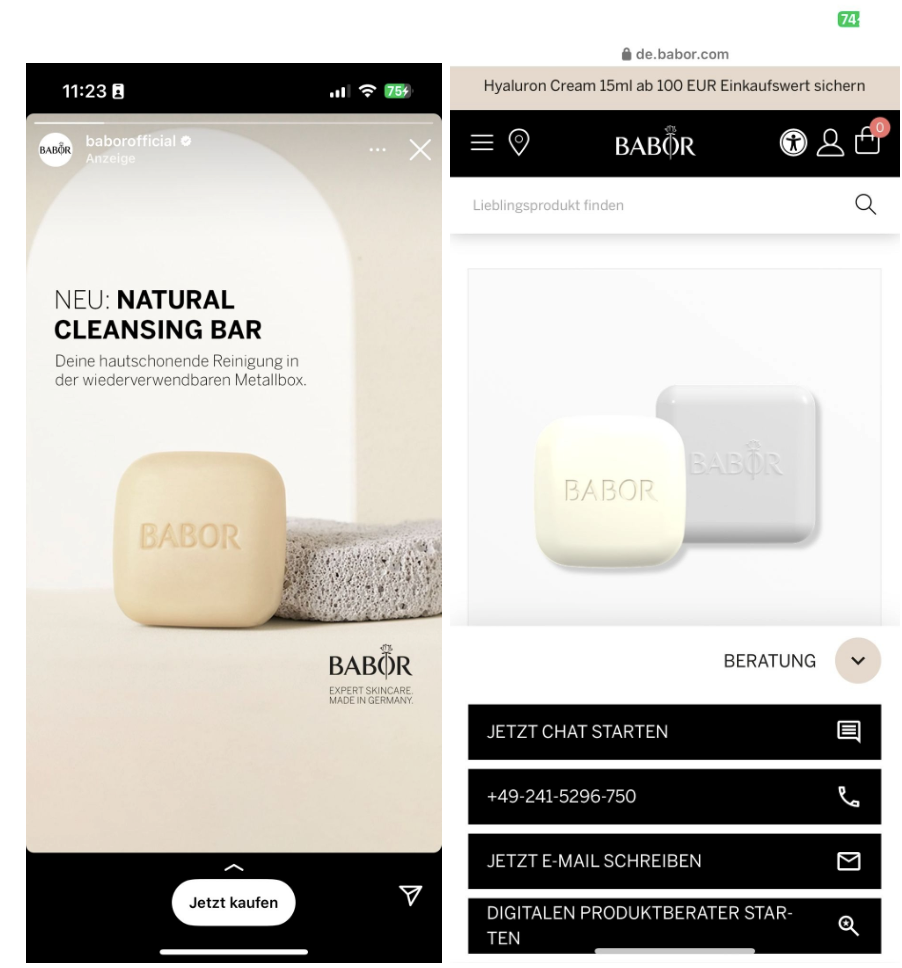
\includegraphics[width=0.7\textwidth]{src/abbildungen/babor_ad.png}
	\caption[Quelle: BABOR Webseite und Instagram AD]{Werbung über Social-Media und Auswahlmöglichkeiten zur Beratung, Quelle: ~\autocite[S.14]{babor2023}}
       \label{fig:Beschreibung}
\end{figure}

In den sozialen Medien versucht BABOR durch regelmäßige Postings, gezielte Werbung und gutes Marketing Aufmerksamkeit auf bestimmte Produkte zu generieren.
\newline
Für ein vorgeschlagenes Produkt wird zudem über den Online-Shop eine Beratung angeboten (z.B. über Telefon, E-Mail oder per Chat) und es kann auch eine eigens entwickelte Hautanalyse, also eine digitale Hautberatung, in Anspruch genommen werden, um das Einkaufserlebnis zu personalisieren und auf jeden Hauttypen empfohlene Produkte zu empfehlen. Zudem besteht die Möglichkeit, durch Cross Selling Produkte anzubieten, die durch das Personalisieren eine erhöhte Wahrscheinlichkeit mit der Übereinstimmung des Kunden oder der Kundin finden. Neukunden erhalten die Möglichkeit, einen Willkommensgutschein in Anspruch zu nehmen, wodurch ein Rabatt bei der ersten Bestellung entsteht. Zudem wird die Möglichkeit angeboten, einen Newsletter zu informieren, bei dem Kunden ihre E-Mail hinterlegen und in regelmäßigen Abständen zur Marke BABOR oder neuen Produkten News oder per E-Mail erhalten.
In der Regel werden zudem bei Bestellungen Gratisproben verteilt, um auf weitere Produkte aufmerksam zu machen.
\newline

Viele BABOR Produkte werden von den Konsumierenden auch über Marktplätze wie Amazon gekauft, weshalb auch BABOR dort sehr aktiv ist und mehrere Key Account Manager eingestellt hat, die sich nur um das Projekt Amazon kümmern. Dort wird zum Beispiel für bestimmte Suchbegriffe auch aktiv Werbung geschaltet, so dass BABOR Produkte in der Kategorie Kosmetik schnell und mit Priorisierung angezeigt werden.
\newline
Über Amazon ist es zum Beispiel möglich, neben den verschiedenen Zahlungsmethoden auch Abonnements für BABOR in verschiedenen Intervallen abzuschließen, so dass ein Produkt in regelmäßigen Abständen automatisch wieder geliefert wird. Zudem garantiert Amazon mit ihrem Prime Angebot eine Gratis Lieferung am nächsten Tag. Durch die große Anzahl an Kosmetikstudios in Deutschland hat sich BABOR deutschlandweit über 2000 Kosmetikpartner herausgesucht, so dass zusätzlich in der Nähe eine Produktberatung in Anspruch genommen werden kann oder Produkte gekauft werden können.
\newline

Bei dem B2B-Geschäft bietet BABOR an die Auftraggebenden weiter einen Fulfillment-Prozess an, bei dem der komplette Logistikprozess von BABOR abgewickelt werden kann.

\subsection{Handlungsempfehlung}\label{hauptabschnitt_5_2}
Unternehmen sollten eine Omni-Channel-Strategie einführen, wenn sie eine bessere Kundenerfahrung und eine höhere Kundenbindung anstreben. Dafür ist es sinnvoll, verschiedene Faktoren zu berücksichtigen.
Unternehmen sollten ihre Kunden und Kundinnen besser verstehen, um festzustellen, wie diese ihre Produkte und Dienstleistungen bevorzugen. Hierfür sollte zum Beispiel das Konzept der Customer Centricity durchgeführt werden, um einen Blick auf die Kundensicht zu erhalten.
\newline

Einige Kunden oder Kundinnen bevorzugen den Kauf über E-Commerce-Websites, andere bevorzugen den Kauf in Geschäften und wiederum andere bevorzugen den Kauf über mobile Apps. Eine Omni-Channel-Strategie ermöglicht es Unternehmen, alle diese Kanäle zu nutzen, um ihre Kunden zu bedienen. Wenn die Konkurrenz bereits eine Omni-Channel-Strategie implementiert hat, kann es sinnvoll sein, ebenfalls eine solche Strategie einzuführen, um wettbewerbsfähig zu bleiben. Eine Omni-Channel-Strategie kann dazu beitragen, dass das Unternehmen eine einheitliche Markendarstellung in allen Kanälen beibehält. Dies trägt dazu bei, die Stärkung des Markenimages herzustellen. Unternehmen sollten auch die Kosten-Nutzen-Analyse durchführen, um festzustellen, ob die Einführung einer Omni-Channel-Strategie für sie wirtschaftlich sinnvoll ist.
\newline

Automatisierung sollte in möglichst vielen Bereichen eingeführt werden, wo es Sinn macht. Beispiele sind immer wieder wiederholende Prozesse. Ein angebotener Self-Service an sich spart Kosten ein und erhöht die Flexibilität der Konsumierenden in den Kontaktpunkten. Die Kosten, die dabei im Self-Service gespart werden, können so in komplexere Themen investiert werden, wie zum Beispiel die Kundenzufriedenheit oder in das Expertenwissen, um auch dort die entsprechenden Kennzahlen optimieren zu können. Durch verbesserte Ausbildungsmöglichkeiten der Mitarbeiter steigt die Expertise in den Fachbereichen und so können schneller, kompetenter und einfacher Lösungen gefunden werden. Gleichzeitig ist es notwendig, verschiedene Kanäle im Kundenkontakt zu nutzen. Dies ist bei weitem noch nicht so verbreitet, wie man es erwarten würde.
\newline

Zudem sollte eine Zielgruppenanalyse  stattfinden, um zu einem Ergebnis zu kommen, welche Kanäle angeboten werden. Wenn das Zielklientel zum Beispiel 65+ ist, sollte das Thema Video-Chat in diesem Bereich nicht das präferierte Hauptziel sein, die Kundschaft anzusprechen. Dabei sollte analysiert werden,  was der Kunde oder die Kundin benötigt und welche Anforderungen gestellt werden.
Auch die Telefonie bleibt ein wichtiger Kanal im persönlichen Kundenkontakt. In diesem Bereich sollten Experten ausgebildet werden, um die Kundschaft erfolgreich und einfach beraten zu können.
\newline

Es gilt auch, Flexibilität in den Kontaktpunkten herzustellen. Die Kunden und Kundinnen wollen nicht permanent mit dem Unternehmen direkt kommunizieren müssen. Falls  jedoch Kommunikation von Seiten des Kunden oder der Kundin gewünscht wird, dann sollten sie die Flexibilität geboten bekommen, den Weg zu entscheiden und dabei schnelle und kompetente Hilfe angeboten bekommen. Im Optimalfall können diese Fragen durch ausgebildetes Expertenwissen beantwortet werden. Um bessere und genauere Entscheidungen treffen zu können, werden für den direkten Kundenkontakt für den Berater entsprechende Kundendaten bereitgestellt, die bei komplexen Themen im persönlichen Kundendialog unterstützen.
\newline

Omni-Channel-Strategien können Unternehmen dabei helfen, ihre Kunden und Kundinnen besser zu bedienen und ihre Kundenerfahrung zu verbessern. Die Einführung einer solchen Strategie erfordert jedoch eine sorgfältige Planung und Umsetzung, um sicherzustellen, dass sie den Bedürfnissen des Unternehmens und seiner Kunden entspricht.

\newpage
\section{Fazit \& Ausblick}\label{hauptabschnitt_6}

Abschließend kann festgestellt werden, dass Omni-Channel für viele Branchen ein wichtiger Trend ist, der es Unternehmen ermöglicht, Konsumierende auf mehreren Kanälen zu erreichen und eine nahtlose und personalisierte Kundenerfahrung zu bieten. Dadurch, dass viele Konsumierende mittlerweile über Smartphone, Tablet, Laptop oder am Computer ihre Einkäufe tätigen oder sich zumindest Informationen zu einem Produkt oder einer Marke einholen, ist die Integration von Online- und Offline-Kanälen entscheidend, um die Kundenbindung zu stärken und den Umsatz zu steigern.
\newline

Die Untersuchungen zeigen, dass die Implementierung von Omni-Channel-Strategien in der Kosmetikbranche noch in den Anfängen steckt und es noch viele Herausforderungen zu bewältigen gibt, wie zum Beispiel die Verwaltung von Bestandsdaten und die Integration von Systemen. Unternehmen, die jedoch erfolgreich eine Omni-Channel-Strategie umsetzen, können eine höhere Kundenbindung und Umsatzsteigerungen erreichen.
\newline

Für zukünftige Forschungsvorhaben könnte es interessant sein, eine tiefere Analyse der Auswirkungen von Omni-Channel auf den Verkauf von Kosmetikprodukten durchzuführen und weitere Faktoren zu berücksichtigen, die die Kundenerfahrung und den Erfolg von Omni-Channel-Strategien beeinflussen. Es könnte auch sinnvoll sein, die Auswirkungen der COVID-19-Pandemie auf die Nutzung von Omni-Channel in der Kosmetikbranche weiter zu untersuchen und mögliche Veränderungen in der Branche zu identifizieren.
\newline

Insgesamt bietet Omni-Channel in der Kosmetikbranche aber viele Chancen, um das Kundenerlebnis zu verbessern und den Erfolg von Unternehmen zu steigern. Unternehmen sollten weiterhin in die Entwicklung und Umsetzung von Omni-Channel-Strategien investieren, um wettbewerbsfähig zu bleiben und auch langfristig erfolgreich zu wirtschaften. Für Unternehmen wird es dabei wichtig sein, auf die Kundenanforderungen einzugehen und sich dabei so auszurichten, dass durch Nutzung neuer Technologien, moderner Softwaresysteme und kreativen Ideen Wettbewerbsvorteile gegenüber der Konkurrenz entstehen können.
\newline

Aus Sicht der stationären Läden wird ein wichtiger Kernpunkt sein, ihre Kundschaft mit einem freundlichen Auftreten und einer ausgewiesenen Expertise bei Produkten zu beraten. Daher ist es wichtig, dass Berater:innen einen Expertenbereich aufbauen, bei dem sie möglichst auf dem neuesten Kenntnisstand sind und ihrer Kundschaft detailliert erklären können, welches Produkt für bestimmte Anforderungen besonders geeignet ist.
\newline

Die Umsetzung einer ganzheitlichen Omni-Channel-Strategie stellt ein Unternehmen vor eine Vielzahl von Herausforderungen. Darunter fallen auch Themen, die aktuell mit Sicherheit noch in den Kinderschuhen stecken. In diesem Zusammenhang steht dem Omni-Channel-Retailing zwar noch eine Wegstrecke bevor, bis es komplett ausgereift ist, aber viele größere Unternehmen in verschiedenen Branchen machen es in Teilen schon vor und sind bereits auf einem sehr guten Weg. Omni-Channel ist ein Geschäftsmodell, das heute bereits Omni-Channel ist ein Geschäftsmodell, das heute bereits bedient und genutzt werden sollte, um in naher Zukunft für den Markt gerüstet zu sein.
\newline

Wenn man die jungen Generationen beobachtet, kann festgestellt werden, wie sich das Kommunikationsverhalten dieser Generationen verändert. Diese Generationen werden diese Trends der Zukunft vorgeben und die Kunden und Kundinnen von morgen sein, die den Unternehmen zeigen, über welche Wege sie kommunizieren wollen. Unternehmen werden sich mittel- und langfristig darauf einstellen müssen, denn wenn das nicht geschieht, besteht die Möglichkeit, den nächsten Klick zu nehmen und ein anderes Zielunternehmen auszuwählen.
\newpage


% Listingverzeichnis anzeigen
% \renewcommand{\lstlistlistingname}{Listingverzeichnis}
% \lstlistoflistings
% \newpage
% \addcontentsline{toc}{section}{Listingverzeichnis}


% Literaturverzeichnis anzeigen
\ohead{Literaturverzeichnis} % Korrektur für Header 
\phantomsection
\addcontentsline{toc}{section}{Literaturverzeichnis}
\renewcommand\refname{Literaturverzeichnis}
%\bibliography{bibtex/Hauptdatei.bib}
\printbibliography
\newpage

% Kein Header für Anhang (Deckblatt) 
%\KOMAoptions{headsepline=false}
%\ohead{}

% Beginn Anhang
%%%%%%%%%%%%%%%%%%%%%%%%%%%%%%%%%%
%      Deckblatt Anhang         %
%%%%%%%%%%%%%%%%%%%%%%%%%%%%%%%%%
\clearpage
\phantomsection
\addcontentsline{toc}{section}{Anhang}
\vspace*{\fill}
\begin{center}
    \doublespacing
    \line(1,0){450}\\
    \textbf{\Huge{Anhang}}\\
    \line(1,0){450}
    \singlespacing
    \begin{verbatim}
      
    \end{verbatim}
    \end{center} 
\vspace*{\fill}
\newpage

% Anhang römisch
%\clearpage
%\renewcommand{\thesection}{\roman{section}}
%\renewcommand{\thesubsection}{\roman{subsection}}
%\setcounter{section}{1}
% Header Anhang (Inhalt)
%\KOMAoptions{headsepline=true}
%\ohead{\headmark}
%\automark{subsection}

% Input Anhang 
%\subsection*{Fragebogen für das Experteninterview}

\subsubsection*{Einleitung}
Vielen Dank, dass Sie sich mit den Fragen im Rahmen meiner Bachelorthesis beschäftigen. Durch die Beantwortung der folgenden Fragen sollen Vor- und Nachteile, aber auch Verbesserungsvorschläge bei der Umsetzung von Omni-Channel-Strategien analysiert werden. Der Fragebogen beschäftigt sich mit der Frage, welche spezifischen Herausforderungen es bei der Implementierung einer Omni-Channel-Strategie im Kosmetikbereich gibt und wie diese speziell von dem Unternehmen BABOR gemeistert bzw. genutzt wurden. Dabei soll herauskristallisiert werden, welche neuen Chancen und Möglichkeiten dabei entstanden sind. Alle Fragen sind freiwillig auszufüllen und sollten Sie bei einer Frage keine Antwort geben können/wollen, kann diese einfach übersprungen werden.

\subsubsection*{Fragen}
\begin{enumerate}
 \item[1.] Bei Omni-Channel-Ansätzen möchte man den Kunden ein möglichst perfektes und rundes Einkaufserlebnis über alle Vertriebskanäle hinweg bieten. Welche Omni-Channel-Konzepte werden bei BABOR eingesetzt?
     \begin{itemize}
            \item{[ ] Click \& Collect}
            \item{[ ] Buy \& Collect}
            \item{[ ] Reserve \& Collect}
            \item{[ ] Weitere Antwortmöglichkeiten:  }
          \end{itemize}
 \item[2.] Welche Vertriebskanäle werden aktuell im B2C genutzt?
     \begin{itemize}
             \item{[ ] Social-Media}
             \item{[ ] Online-Shop}
             \item{[ ] Stationärer Handel}
             \item{[ ] Weitere Antwortmöglichkeiten:  }
           \end{itemize}
 \item[3.] Welche Vertriebskanäle werden aktuell im B2B genutzt?
    \begin{itemize}
              \item{[ ] Social-Media}
              \item{[ ] Online-Shop}
              \item{[ ] Andere Vertriebskanäle}
              \item{[ ] Weitere Antwortmöglichkeiten:  }
            \end{itemize}
 \item[4.] Über welche Berührungspunkte (Touchpoints) kommen die Kunden (B2B als auch B2C) mit dem Unternehmen oder der Marke BABOR in Kontakt?
    \begin{itemize}
               \item{[ ] Broschüre}
               \item{[ ] Print}
               \item{[ ] Pressearbeit}
               \item{[ ] Online-Anzeigen}
               \item{[ ] Social-Media-Werbung}
               \item{[ ] Newsletter}
               \item{[ ] Community / Social-Media}
               \item{[ ] Filialgeschäft}
               \item{[ ] Weitere Antwortmöglichkeiten:  }
             \end{itemize}
 \item[5.] Als Familienunternehmen wurde bei BABOR lange Zeit das B2B Modell in den Mittelpunkt gestellt. Was waren die Gründe für eine Veränderung der Marketing-Strategie zum B2C?
 \item[6.] Was sind die relevantesten Kontaktpunkte mit Kunden, bei denen Informationen über den Kunden gewonnen werden und denen die größte Aufmerksamkeit geschenkt wird?
 \item[7.] BABOR Produkte sind in vielen Kosmetikstudios sehr beliebt. Trotzdem setzt BABOR mittlerweile vermehrt auch auf das B2C-Vertriebsmodell und den Onlinehandel. Welche Prozessveränderungen gab es bei der Umsetzung der neuen Strategieausrichtung?
 \item[8.] Welche Omni-Channel-Ansätze wurden bei dieser Entscheidung berücksichtigt und spielten dabei eine wichtige Rolle?
 \item[9.] Wenn es zu marketingtechnischen Veränderungen kommt, kann dies oftmals auch ein mehrjähriger Prozess sein. Welcher Aufwand war für den Prozess bei BABOR erforderlich, um sich neu auszurichten?
 \item[10.] Welche technischen Prozesse oder Systeme (z.B. neues CRM-System) wurden für die Umsetzung einer Omni-Channel-Strategie grundlegend neu eingeführt und umgesetzt?
 \item[11.] Wenn ein komplett neues CRM-System integriert wird, wird z.B. für die Datenpflege ein sehr hoher Aufwand erwartet. Sind in diesem Zusammenhang bei der Einführung von Systemen irgendwelche (unerwarteten) Probleme entstanden?
 \item[12.] Durch Instagram besteht die Möglichkeit, global eine Reichweite zu generieren. In der Kosmetik-Branche werden auch von Influencern immer wieder Werbung für ein Produkt oder eine Marke veröffentlicht. Welche Vorteile entstehen bei BABOR durch diese Vertriebskanäle und wofür werden diese hauptsächlich genutzt?
    \begin{itemize}
               \item{[ ] Informations- und Anleitungsvideos zu Produkten}
               \item{[ ] Werbung für neue Produkte}
               \item{[ ] Auf die Marke BABOR aufmerksam machen wollen}
               \item{[ ] Weitere Antwortmöglichkeiten:  }
             \end{itemize}
 \item[13.] BABOR Produkte sind bei vielen Kosmetikstudios nach wie vor sehr beliebt. Entsteht durch den Online-Shop eine Zielgruppen-Veränderung oder Zielgruppen-Erweiterung für das Unternehmen? Und was möchte BABOR neben einem guten Produkt tun, um diese Zielgruppen erfolgreich zu erreichen und zufriedenzustellen?
 \item[14.] Über welchen Vertriebskanal wird bei BABOR der größte Umsatz generiert und was wird getan, um das Einkaufserlebnis des Kunden/der Kundin angenehmer zu gestalten?
 \item[15.] Wenn bei einer Parfümerie wie Douglas nach einem BABOR Produkt gesucht wird, gibt es die Möglichkeit, Strategien zu verfolgen, das Einkaufserlebnis für den Kunden oder der Kundin angenehmer zu gestalten? Beispielsweise über einen QR-Code auf dem Produkt, das als Video eine Anleitung zeigt.
 \item[16.] Kann auch von Unternehmen gelernt werden, die in ganz anderen Bereichen/Branchen tätig sind? Wird dabei zum Beispiel auch auf die Big Player wie Amazon geachtet?
 \item[17.] Wie sieht die generelle Marktentwicklung in der Kosmetikbranche und insbesondere bei den Hauptkonkurrenten aus und welche Tendenzen lassen sich für BABOR ableiten?
 \item[18.] Während der Lockdowns aus der Corona-Zeit wurde in vielen Branchen (zum Teil auch notgedrungen) vermehrt auf das Einkaufen im Online-Handel gesetzt. Gab es durch die Zeit der Corona-Pandemie spürbare Veränderungen der Konsumierenden in Bezug auf das Einkaufsverhalten?
 \item[19.] Wenn ja, inwieweit wird versucht, das zu berücksichtigen?
\end{enumerate}
%\newpage

% Eidesstattliche Erklärung
\phantomsection
\addcontentsline{toc}{section}{Eidesstattliche Erklärung}

% Header für Erklärung
\ohead{Eidesstattliche Erklärung}

% Input Erklärung
\section*{Eidesstattliche Erklärung}

\vspace{1cm}
Ich versichere, die von mir vorgelegte Arbeit selbstständig verfasst zu haben. Alle Stellen, die wörtlich oder sinngemäß aus veröffentlichten oder nicht veröffentlichten Arbeiten anderer entnommen sind, 
habe ich als entnommen kenntlich gemacht. Sämtliche Quellen und Hilfsmittel, die ich für die Arbeit benutzt habe, sind angegeben. Die Arbeit hat mit gleichem Inhalt bzw. in wesentlichen 
Teilen noch keiner anderen Prüfungsbehörde vorgelegen.



\begin{displaymath}
\begin{array}{ll}
Unterschrift:~~~~~~~~~~~~~~~~~~~~~~~~~~~~~~~~~~~~~~~~~~
& Ort, Datum:~~~~~~~~~~~~~~~~~~~~~~~~~~~~~~~~~~~~~~~~~~
\end{array}
\end{displaymath}


% Leere Abschlussseite
\newpage
\thispagestyle{empty} % erzeugt Seite ohne Kopf- / Fusszeile
\mbox{}

\end{document}
